%\clearpage
%\subsection{Background Uncertainties}
\label{subsec:bkg_uncer}

%%%	
Several systematic uncertainties associated with the modeling of backgrounds have been assessed. These uncertainties include a shape systematic related to the discriminant used in the analysis and a normalization systematic for predictions derived solely from simulations.
The complete list of the alternative samples utilized to derive these background uncertainties is provided in the Tables
\ref{tabular:mc_samples_alt_Wenujets}-\ref{tabular:mc_samples_alt_ttbar}.

%%% alternative bkg samples
\begin{table}[p]
\caption{$W \to e\nu$+jets alternative samples used in the analysis. The dataset ID, MC generator, production cross section, filter efficiency and total number of generated events are shown.}
\label{tabular:mc_samples_alt_Wenujets}
\begin{footnotesize}
\begin{center}
\begin{tabular}{c|l|c|c|c}
  \hline
  DS ID & Name & $\sigma\times\text{BR}$ [pb] & k-factor & $\epsilon_{\text{filter}}$ \\ \hline
363600  & MGPy8EG\_N30NLO\_Wenu\_Ht0\_70\_CVetoBVeto            & 16719.0                      & 1.12      & 8.38E+03 \\
363601  & MGPy8EG\_N30NLO\_Wenu\_Ht0\_70\_CFilterBVeto          & 16720.0                      & 1.12      & 1.38E+03 \\
363602  & MGPy8EG\_N30NLO\_Wenu\_Ht0\_70\_BFilter               & 16717.0                      & 1.12      & 2.42E+02 \\
363603  & MGPy8EG\_N30NLO\_Wenu\_Ht70\_140\_CVetoBVeto          & 755.1                        & 1.12      & 7.12E+03 \\
363604  & MGPy8EG\_N30NLO\_Wenu\_Ht70\_140\_CFilterBVeto        & 755.77                       & 1.12      & 2.40E+03 \\
363605  & MGPy8EG\_N30NLO\_Wenu\_Ht70\_140\_BFilter             & 755.73                       & 1.12      & 4.83E+02 \\
363606  & MGPy8EG\_N30NLO\_Wenu\_Ht140\_280\_CVetoBVeto         & 318.96                       & 1.12      & 6.66E+03 \\
363607  & MGPy8EG\_N30NLO\_Wenu\_Ht140\_280\_CFilterBVeto       & 319.93                       & 1.12      & 2.64E+03 \\
363608  & MGPy8EG\_N30NLO\_Wenu\_Ht140\_280\_BFilter            & 319.45                       & 1.12      & 6.94E+02 \\
363609  & MGPy8EG\_N30NLO\_Wenu\_Ht280\_500\_CVetoBVeto         & 73.528                       & 1.12      & 6.19E+03 \\
363610  & MGPy8EG\_N30NLO\_Wenu\_Ht280\_500\_CFilterBVeto       & 73.562                       & 1.12      & 2.85E+03 \\
363611  & MGPy8EG\_N30NLO\_Wenu\_Ht280\_500\_BFilter            & 73.556                       & 1.12      & 9.52E+02 \\
363612  & MGPy8EG\_N30NLO\_Wenu\_Ht500\_700\_CVetoBVeto         & 11.529                       & 1.12      & 5.87E+03 \\
363613  & MGPy8EG\_N30NLO\_Wenu\_Ht500\_700\_CFilterBVeto       & 11.517                       & 1.12      & 2.98E+03 \\
363614  & MGPy8EG\_N30NLO\_Wenu\_Ht500\_700\_BFilter            & 11.51                        & 1.12      & 1.15E+03 \\
363615  & MGPy8EG\_N30NLO\_Wenu\_Ht700\_1000\_CVetoBVeto        & 40.158                       & 1.12      & 5.66E+03 \\
363616  & MGPy8EG\_N30NLO\_Wenu\_Ht700\_1000\_CFilterBVeto      & 4.014                        & 1.12      & 3.04E+03 \\
363617  & MGPy8EG\_N30NLO\_Wenu\_Ht700\_1000\_BFilter           & 40.123                       & 1.12      & 1.28E+03 \\
363618  & MGPy8EG\_N30NLO\_Wenu\_Ht1000\_2000\_CVetoBVeto       & 13.243                       & 1.12      & 5.48E+03 \\
363619  & MGPy8EG\_N30NLO\_Wenu\_Ht1000\_2000\_CFilterBVeto     & 13.286                       & 1.12      & 3.08E+03 \\
363620  & MGPy8EG\_N30NLO\_Wenu\_Ht1000\_2000\_BFilter          & 1.326                        & 1.12      & 1.43E+03 \\
363621  & MGPy8EG\_N30NLO\_Wenu\_Ht2000\_E\_CMS\_CVetoBVeto      & 0.042294                     & 1.12      & 5.24E+03 \\
363622  & MGPy8EG\_N30NLO\_Wenu\_Ht2000\_E\_CMS\_CFilterBVeto    & 0.041884                     & 1.12      & 3.17E+03 \\
363623  & MGPy8EG\_N30NLO\_Wenu\_Ht2000\_E\_CMS\_BFilter         & 0.047382                     & 1.12      & 1.51E+03 \\
\hline
\end{tabular}
\end{center}
\end{footnotesize}
\end{table}

\begin{table}[p]
\caption{$W \to \mu\nu$+jets alternative samples used in the analysis. The dataset ID, MC generator, production cross section, filter efficiency and total number of generated events are shown.}
\label{tabular:mc_samples_alt_Wmunujets}
\begin{footnotesize}
\begin{center}
\begin{tabular}{c|l|c|c|c}
  \hline
  DS ID & Name & $\sigma\times\text{BR}$ [pb] & k-factor & $\epsilon_{\text{filter}}$ \\ \hline
363624  & MGPy8EG\_N30NLO\_Wmunu\_Ht0\_70\_CVetoBVeto         & 16720.0                    &  1.12   &       8.38E+03        \\
363625  & MGPy8EG\_N30NLO\_Wmunu\_Ht0\_70\_CFilterBVeto       & 16717.0                    &  1.12   &       1.38E+03        \\
363626  & MGPy8EG\_N30NLO\_Wmunu\_Ht0\_70\_BFilter            & 16719.0                    &  1.12   &       2.42E+02        \\
363627  & MGPy8EG\_N30NLO\_Wmunu\_Ht70\_140\_CVetoBVeto       & 755.19                     &  1.12   &       7.12E+03        \\
363628  & MGPy8EG\_N30NLO\_Wmunu\_Ht70\_140\_CFilterBVeto     & 755.62                     &  1.12   &       2.40E+03        \\
363629  & MGPy8EG\_N30NLO\_Wmunu\_Ht70\_140\_BFilter          & 755.77                     &  1.12   &       4.83E+02        \\
363630  & MGPy8EG\_N30NLO\_Wmunu\_Ht140\_280\_CVetoBVeto      & 318.83                     &  1.12   &       6.66E+03        \\
363631  & MGPy8EG\_N30NLO\_Wmunu\_Ht140\_280\_CFilterBVeto    & 319.89                     &  1.12   &       2.64E+03        \\
363632  & MGPy8EG\_N30NLO\_Wmunu\_Ht140\_280\_BFilter         & 319.41                     &  1.12   &       6.94E+02        \\
363633  & MGPy8EG\_N30NLO\_Wmunu\_Ht280\_500\_CVetoBVeto      & 73.585                     &  1.12   &       6.19E+03        \\
363634  & MGPy8EG\_N30NLO\_Wmunu\_Ht280\_500\_CFilterBVeto    & 73.548                     &  1.12   &       2.85E+03        \\
363635  & MGPy8EG\_N30NLO\_Wmunu\_Ht280\_500\_BFilter         & 73.569                     &  1.12   &       9.52E+02        \\
363636  & MGPy8EG\_N30NLO\_Wmunu\_Ht500\_700\_CVetoBVeto      & 11.522                     &  1.12   &       5.86E+03        \\
363637  & MGPy8EG\_N30NLO\_Wmunu\_Ht500\_700\_CFilterBVeto    & 11.524                     &  1.12   &       2.96E+03        \\
363638  & MGPy8EG\_N30NLO\_Wmunu\_Ht500\_700\_BFilter         & 11.522                     &  1.12   &       1.16E+03        \\
363639  & MGPy8EG\_N30NLO\_Wmunu\_Ht700\_1000\_CVetoBVeto     & 40.194                     &  1.12   &       5.67E+03        \\
363640  & MGPy8EG\_N30NLO\_Wmunu\_Ht700\_1000\_CFilterBVeto   & 40.252                     &  1.12   &       3.05E+03        \\
363641  & MGPy8EG\_N30NLO\_Wmunu\_Ht700\_1000\_BFilter        & 40.139                     &  1.12   &       1.28E+03        \\
363642  & MGPy8EG\_N30NLO\_Wmunu\_Ht1000\_2000\_CVetoBVeto    & 13.262                     &  1.12   &       5.45E+03        \\
363643  & MGPy8EG\_N30NLO\_Wmunu\_Ht1000\_2000\_CFilterBVeto  & 13.215                     &  1.12   &       3.08E+03        \\
363644  & MGPy8EG\_N30NLO\_Wmunu\_Ht1000\_2000\_BFilter       & 13.287                     &  1.12   &       1.44E+03        \\
363645  & MGPy8EG\_N30NLO\_Wmunu\_Ht2000\_E\_CMS\_CVetoBVeto   & 0.041697                   &  1.12   &       5.20E+03        \\
363646  & MGPy8EG\_N30NLO\_Wmunu\_Ht2000\_E\_CMS\_CFilterBVeto & 0.042199                   &  1.12   &       3.17E+03        \\
363647  & MGPy8EG\_N30NLO\_Wmunu\_Ht2000\_E\_CMS\_BFilter      & 0.042049                   &  1.12   &       1.59E+03        \\
\hline
\end{tabular}
\end{center}
\end{footnotesize}
\end{table}

\begin{table}[p]
\caption{$W \to \tau\nu$+jets alternative samples used in the analysis. The dataset ID, MC generator, production cross section, filter efficiency and total number of generated events are shown.}
\label{tabular:mc_samples_alt_Wtaunujets}
\begin{footnotesize}
\begin{center}
\begin{tabular}{c|l|c|c|c}
  \hline
  DS ID & Name & $\sigma\times\text{BR}$ [pb] & k-factor & $\epsilon_{\text{filter}}$ \\ \hline
363648  & MGPy8EG\_N30NLO\_Wtaunu\_Ht0\_70\_CVetoBVeto        & 16702.0                    &  1.12   &       8.38E+03        \\
363649  & MGPy8EG\_N30NLO\_Wtaunu\_Ht0\_70\_CFilterBVeto      & 16702.0                    &  1.12   &       1.38E+03        \\
363650  & MGPy8EG\_N30NLO\_Wtaunu\_Ht0\_70\_BFilter           & 16702.0                    &  1.12   &       2.42E+02        \\
363651  & MGPy8EG\_N30NLO\_Wtaunu\_Ht70\_140\_CVetoBVeto      & 754.91                     &  1.12   &       7.12E+03        \\
363652  & MGPy8EG\_N30NLO\_Wtaunu\_Ht70\_140\_CFilterBVeto    & 755.3                      &  1.12   &       2.39E+03        \\
363653  & MGPy8EG\_N30NLO\_Wtaunu\_Ht70\_140\_BFilter         & 755.14                     &  1.12   &       4.85E+02        \\
363654  & MGPy8EG\_N30NLO\_Wtaunu\_Ht140\_280\_CVetoBVeto     & 315.31                     &  1.12   &       6.67E+03        \\
363655  & MGPy8EG\_N30NLO\_Wtaunu\_Ht140\_280\_CFilterBVeto   & 316.05                     &  1.12   &       2.64E+03        \\
363656  & MGPy8EG\_N30NLO\_Wtaunu\_Ht140\_280\_BFilter        & 315.64                     &  1.12   &       6.93E+02        \\
363657  & MGPy8EG\_N30NLO\_Wtaunu\_Ht280\_500\_CVetoBVeto     & 72.275                     &  1.12   &       6.22E+03        \\
363658  & MGPy8EG\_N30NLO\_Wtaunu\_Ht280\_500\_CFilterBVeto   & 72.19                      &  1.12   &       2.85E+03        \\
363659  & MGPy8EG\_N30NLO\_Wtaunu\_Ht280\_500\_BFilter        & 72.226                     &  1.12   &       9.52E+02        \\
363660  & MGPy8EG\_N30NLO\_Wtaunu\_Ht500\_700\_CVetoBVeto     & 11.44                      &  1.12   &       5.88E+03        \\
363661  & MGPy8EG\_N30NLO\_Wtaunu\_Ht500\_700\_CFilterBVeto   & 11.463                     &  1.12   &       2.97E+03        \\
363662  & MGPy8EG\_N30NLO\_Wtaunu\_Ht500\_700\_BFilter        & 11.459                     &  1.12   &       1.16E+03        \\
363663  & MGPy8EG\_N30NLO\_Wtaunu\_Ht700\_1000\_CVetoBVeto    & 40.265                     &  1.12   &       5.67E+03        \\
363664  & MGPy8EG\_N30NLO\_Wtaunu\_Ht700\_1000\_CFilterBVeto  & 4.027                      &  1.12   &       3.03E+03        \\
363665  & MGPy8EG\_N30NLO\_Wtaunu\_Ht700\_1000\_BFilter       & 40.283                     &  1.12   &       1.30E+03        \\
363666  & MGPy8EG\_N30NLO\_Wtaunu\_Ht1000\_2000\_CVetoBVeto   & 13.264                     &  1.12   &       5.46E+03        \\
363667  & MGPy8EG\_N30NLO\_Wtaunu\_Ht1000\_2000\_CFilterBVeto & 13.205                     &  1.12   &       3.12E+03        \\
363668  & MGPy8EG\_N30NLO\_Wtaunu\_Ht1000\_2000\_BFilter      & 13.222                     &  1.12   &       1.43E+03        \\
363669  & MGPy8EG\_N30NLO\_Wtaunu\_Ht2000\_E\_CMS\_CVetoBVeto  & 0.043501                   &  1.12   &       5.21E+03        \\
363670  & MGPy8EG\_N30NLO\_Wtaunu\_Ht2000\_E\_CMS\_CFilterBVeto  &                          0.042721  &       1.12            & 3.18E+03 \\
363671  & MGPy8EG\_N30NLO\_Wtaunu\_Ht2000\_E\_CMS\_BFilter       &                          0.042683  &       1.12            & 1.66E+03 \\
\hline
\end{tabular}
\end{center}
\end{footnotesize}
\end{table}

\begin{table}[p]
\caption{$Z \to ee$+jets alternative samples used in the analysis. The dataset ID, MC generator, production cross section, filter efficiency and total number of generated events are shown.}
\label{tabular:mc_samples_alt_Zeejets}
\begin{footnotesize}
\begin{center}
\begin{tabular}{c|l|c|c|c}
  \hline
  DS ID & Name & $\sigma\times\text{BR}$ [pb] & k-factor & $\epsilon_{\text{filter}}$ \\ \hline
363147  & MGPy8EG\_N30NLO\_Zee\_Ht0\_70\_CVetoBVeto  &        1719.7                       &  1.141  &       0.83292 \\
363148  & MGPy8EG\_N30NLO\_Zee\_Ht0\_70\_CFilterBVeto         &                            1719.4    &       1.141   &       0.10775 \\
363149  & MGPy8EG\_N30NLO\_Zee\_Ht0\_70\_BFilter              &                            1719.4    &       1.141   &       0.059156 \\
363150  & MGPy8EG\_N30NLO\_Zee\_Ht70\_140\_CVetoBVeto         &                            85.105    &       1.141   &       0.71754  \\
363151  & MGPy8EG\_N30NLO\_Zee\_Ht70\_140\_CFilterBVeto       &                            85.041    &       1.141   &       0.17377  \\
363152  & MGPy8EG\_N30NLO\_Zee\_Ht70\_140\_BFilter            &                            85.175    &       1.141   &       0.10763  \\
363153  & MGPy8EG\_N30NLO\_Zee\_Ht140\_280\_CVetoBVeto        &                            36.005    &       1.141   &       0.67279  \\
363154  & MGPy8EG\_N30NLO\_Zee\_Ht140\_280\_CFilterBVeto      &                            36.028    &       1.141   &       0.19996  \\
363155  & MGPy8EG\_N30NLO\_Zee\_Ht140\_280\_BFilter           &                            36.06     &       1.141   &       0.12486  \\
363156  & MGPy8EG\_N30NLO\_Zee\_Ht280\_500\_CVetoBVeto        &                            82.054    &       1.141   &       0.62846  \\
363157  & MGPy8EG\_N30NLO\_Zee\_Ht280\_500\_CFilterBVeto      &                            82.126    &       1.141   &       0.22726  \\
363158  & MGPy8EG\_N30NLO\_Zee\_Ht280\_500\_BFilter           &                            82.474    &       1.141   &       0.14193  \\
363159  & MGPy8EG\_N30NLO\_Zee\_Ht500\_700\_CVetoBVeto        &                            12.733    &       1.141   &       0.5966   \\
363160  & MGPy8EG\_N30NLO\_Zee\_Ht500\_700\_CFilterBVeto      &                            1.273     &       1.141   &       0.24847  \\
363161  & MGPy8EG\_N30NLO\_Zee\_Ht500\_700\_BFilter           &                            12.722    &       1.141   &       0.15256  \\
363162  & MGPy8EG\_N30NLO\_Zee\_Ht700\_1000\_CVetoBVeto       &                            0.44546   &       1.141   &       0.57676  \\
363163  & MGPy8EG\_N30NLO\_Zee\_Ht700\_1000\_CFilterBVeto     &                            0.44611   &       1.141   &       0.26137  \\
363164  & MGPy8EG\_N30NLO\_Zee\_Ht700\_1000\_BFilter          &                            0.44603   &       1.141   &       0.16181  \\
363165  & MGPy8EG\_N30NLO\_Zee\_Ht1000\_2000\_CVetoBVeto      &                            0.15208   &       1.141   &       0.55543  \\
363166  & MGPy8EG\_N30NLO\_Zee\_Ht1000\_2000\_CFilterBVeto    &                            0.15248   &       1.141   &       0.27476  \\
363167  & MGPy8EG\_N30NLO\_Zee\_Ht1000\_2000\_BFilter         &                            0.15327   &       1.141   &       0.16618  \\
363168  & MGPy8EG\_N30NLO\_Zee\_Ht2000\_E\_CMS\_CVetoBVeto     &                            0.0056989 &       1.141   &       0.53136  \\
363169  & MGPy8EG\_N30NLO\_Zee\_Ht2000\_E\_CMS\_CFilterBVeto   &                            0.0057408 &       1.141   &       0.2923   \\
363170  & MGPy8EG\_N30NLO\_Zee\_Ht2000\_E\_CMS\_BFilter        &                            0.0057164 &       1.141   &       0.17489  \\
\hline
\end{tabular}
\end{center}
\end{footnotesize}
\end{table}

\begin{table}[p]
\caption{$Z \to \mu\mu$+jets alternative samples used in the analysis. The dataset ID, MC generator, production cross section, filter efficiency and total number of generated events are shown.}
\label{tabular:mc_samples_alt_Zmumujets}
\begin{footnotesize}
\begin{center}
\begin{tabular}{c|l|c|c|c}
  \hline
  DS ID & Name & $\sigma\times\text{BR}$ [pb] & k-factor & $\epsilon_{\text{filter}}$ \\ \hline
363123  & MGPy8EG\_N30NLO\_Zmumu\_Ht0\_70\_CVetoBVeto         & 1714.5                     &  1.141  &       0.83157 \\
363124  & MGPy8EG\_N30NLO\_Zmumu\_Ht0\_70\_CFilterBVeto       & 1715.5                     &  1.141  &       0.10835 \\
363125  & MGPy8EG\_N30NLO\_Zmumu\_Ht0\_70\_BFilter            & 1715.7                     &  1.141  &       0.059162        \\
363126  & MGPy8EG\_N30NLO\_Zmumu\_Ht70\_140\_CVetoBVeto       & 84.57                      &  1.141  &       0.71809         \\
363127  & MGPy8EG\_N30NLO\_Zmumu\_Ht70\_140\_CFilterBVeto     & 84.588                     &  1.141  &       0.17404         \\
363128  & MGPy8EG\_N30NLO\_Zmumu\_Ht70\_140\_BFilter          & 84.752                     &  1.141  &       0.10804         \\
363129  & MGPy8EG\_N30NLO\_Zmumu\_Ht140\_280\_CVetoBVeto      & 35.883                     &  1.141  &       0.67432         \\
363130  & MGPy8EG\_N30NLO\_Zmumu\_Ht140\_280\_CFilterBVeto    & 35.908                     &  1.141  &       0.19951         \\
363131  & MGPy8EG\_N30NLO\_Zmumu\_Ht140\_280\_BFilter         & 35.887                     &  1.141  &       0.12607         \\
363132  & MGPy8EG\_N30NLO\_Zmumu\_Ht280\_500\_CVetoBVeto      & 81.871                     &  1.141  &       0.62802         \\
363133  & MGPy8EG\_N30NLO\_Zmumu\_Ht280\_500\_CFilterBVeto    & 81.805                     &  1.141  &       0.2282          \\
363134  & MGPy8EG\_N30NLO\_Zmumu\_Ht280\_500\_BFilter         & 81.705                     &  1.141  &       0.14263         \\
363135  & MGPy8EG\_N30NLO\_Zmumu\_Ht500\_700\_CVetoBVeto      & 1.271                      &  1.141  &       0.59722         \\
363136  & MGPy8EG\_N30NLO\_Zmumu\_Ht500\_700\_CFilterBVeto    & 12.672                     &  1.141  &       0.24952         \\
363137  & MGPy8EG\_N30NLO\_Zmumu\_Ht500\_700\_BFilter         & 12.699                     &  1.141  &       0.15292         \\
363138  & MGPy8EG\_N30NLO\_Zmumu\_Ht700\_1000\_CVetoBVeto     & 0.43601                    &  1.141  &       0.57118         \\
363139  & MGPy8EG\_N30NLO\_Zmumu\_Ht700\_1000\_CFilterBVeto   & 0.44623                    &  1.141  &       0.25948         \\
363140  & MGPy8EG\_N30NLO\_Zmumu\_Ht700\_1000\_BFilter        & 0.44567                    &  1.141  &       0.15965         \\
363141  & MGPy8EG\_N30NLO\_Zmumu\_Ht1000\_2000\_CVetoBVeto    & 0.14899                    &  1.141  &       0.54908         \\
363142  & MGPy8EG\_N30NLO\_Zmumu\_Ht1000\_2000\_CFilterBVeto  & 0.14625                    &  1.141  &       0.27164         \\
363143  & MGPy8EG\_N30NLO\_Zmumu\_Ht1000\_2000\_BFilter       & 0.14705                    &  1.141  &       0.17299         \\
363144  & MGPy8EG\_N30NLO\_Zmumu\_Ht2000\_E\_CMS\_CVetoBVeto   & 0.005538                   &  1.141  &       0.56337         \\
363145  & MGPy8EG\_N30NLO\_Zmumu\_Ht2000\_E\_CMS\_CFilterBVet  & 0.0055466                  &  1.141  &       0.29294         \\
363146  & MGPy8EG\_N30NLO\_Zmumu\_Ht2000\_E\_CMS\_BFilter      & 0.0056422                  &  1.141  &       0.16307         \\
\hline
\end{tabular}
\end{center}
\end{footnotesize}
\end{table}

\begin{table}[p]
\caption{$Z \to \nu\nu$+jets alternative samples used in the analysis. The dataset ID, MC generator, production cross section, filter efficiency and total number of generated events are shown.}
\label{tabular:mc_samples_alt_Znunujets}
\begin{footnotesize}
\begin{center}
\begin{tabular}{c|l|c|c|c}
  \hline
  DS ID & Name & $\sigma\times\text{BR}$ [pb] & k-factor & $\epsilon_{\text{filter}}$ \\ \hline
361515  & MadGraphPythia8EvtGen\_A14NNPDF23LO\_Znunu\_Np0              &  7518.4 &       12.283  &       1.0 \\
361516  & MadGraphPythia8EvtGen\_A14NNPDF23LO\_Znunu\_Np1              &  1200.1 &       12.283  &       1.0 \\
361517  & MadGraphPythia8EvtGen\_A14NNPDF23LO\_Znunu\_Np2              &  387.16 &       12.283  &       1.0 \\
361518  & MadGraphPythia8EvtGen\_A14NNPDF23LO\_Znunu\_Np3              &  110.08 &       12.283  &       1.0 \\
361519  & 361519.MadGraphPythia8EvtGen\_A14NNPDF23LO\_Znunu\_Np4              &  43.389 &       12.283  &       1.0 \\
\hline
\end{tabular}
\end{center}
\end{footnotesize}
\end{table}

\begin{table}[p]
\caption{$t\bar{t}$ alternative samples used in the analysis. The dataset ID, MC generator, production cross section, filter efficiency and total number of generated events are shown.}
\label{tabular:mc_samples_alt_ttbar}
\begin{footnotesize}
\begin{center}
\begin{tabular}{c|l|c|c|c}
  \hline
  DS ID & Name & $\sigma\times\text{BR}$ [pb] & k-factor & $\epsilon_{\text{filter}}$ \\ \hline
410465  & aMcAtNloPy8EvtGen\_MEN30NLO\_A14N23LO\_ttbar\_noShWe\_dil                        &  712.02 &       11.681  &       1.07E+03 \\
410464  & aMcAtNloPy8EvtGen\_MEN30NLO\_A14N23LO\_ttbar\_noShWe\_SingleLep                  &  711.43 &       11.691  &       4.40E+03 \\
410467  & PhPy8EG\_A14\_ttbar\_hdamp517p5\_nonallhad\_AK10J160                             &  729.74 &       1.0     &       1.56E+03 \\
410468  & PowhegHerwig7EG\_H7UE\_tt\_hdamp258p75\_704\_nonallhad\_AK10J160                  &  730.15 &       1.0     &       1.50E+03 \\
410469  & aMcAtNloPy8EG\_MEN30NLO\_A14N23LO\_ttbar\_nonallhad\_AK10J160                    &  711.41 &       1.0     &       1.42E+03 \\
410480  & PhPy8EG\_A14\_ttbar\_hdamp517p5\_SingleLep                                      &  729.74 &       1.0     &       4.39E+03 \\
410482  & PhPy8EG\_A14\_ttbar\_hdamp517p5\_dil                                            &  729.74 &       1.0     &       1.05E+03 \\
410557  & PowhegHerwig7EvtGen\_H7UE\_tt\_hdamp258p75\_704\_SingleLep                       &  730.14 &       1.0     &       4.39E+03 \\
410558  & PowhegHerwig7EvtGen\_H7UE\_tt\_hdamp258p75\_704\_dil                             &  730.15 &       1.0     &       1.05E+03 \\
\hline
\end{tabular}
\end{center}
\end{footnotesize}
\end{table}

%For scale and pdf uncertainties, see \ref{subsec:sig_uncer}.

%%%
\clearpage
\subsection{PDF and Scale uncertainties}
\label{subsec:scale_pdf_unc}

The uncertainties related to Parton Distribution Functions (PDFs), which include alternative PDF sets and variations in the strong coupling constant $\alpha_s$, are addressed following the guidelines from the Physics Modelling Group (PMG).
An envelope encompassing these variations is designated as the PDF uncertainty.
Examples involving alternative PDFs are presented in Figure \ref{fig:extPDFUnc1Lep},
and impacts of combined NNPDF and $\alpha_s$ uncertainties are shown in Figure \ref{fig:PDFUnc1Lep_bkg}.
The uncertainty is determined by using the standard deviation of the mean values from the 100 MC replicas of the NNPDF set for each bin of the considered distributions.

The scale uncertainty associated with the renormalisation ($\mu_r$) and factorisation ($\mu_f$) scales is determined by the envelope of variations. 
These variations arise from independently scaling $\mu_r$ and $\mu_f$ by factors of 2 and 0.5, 
excluding the extreme cases of multiplying $\mu_r$ by 2 and $\mu_f$ by 0.5, and vice versa.
The combined results of these variations are shown in Figures \ref{fig:PDFUnc1Lep_QCD}.

%%An envelope of these various variations is taken as "PDF uncertainty".

\begin{figure}[ht]
    \centering
    \begin{subfigure}[b]{0.3\textwidth}
        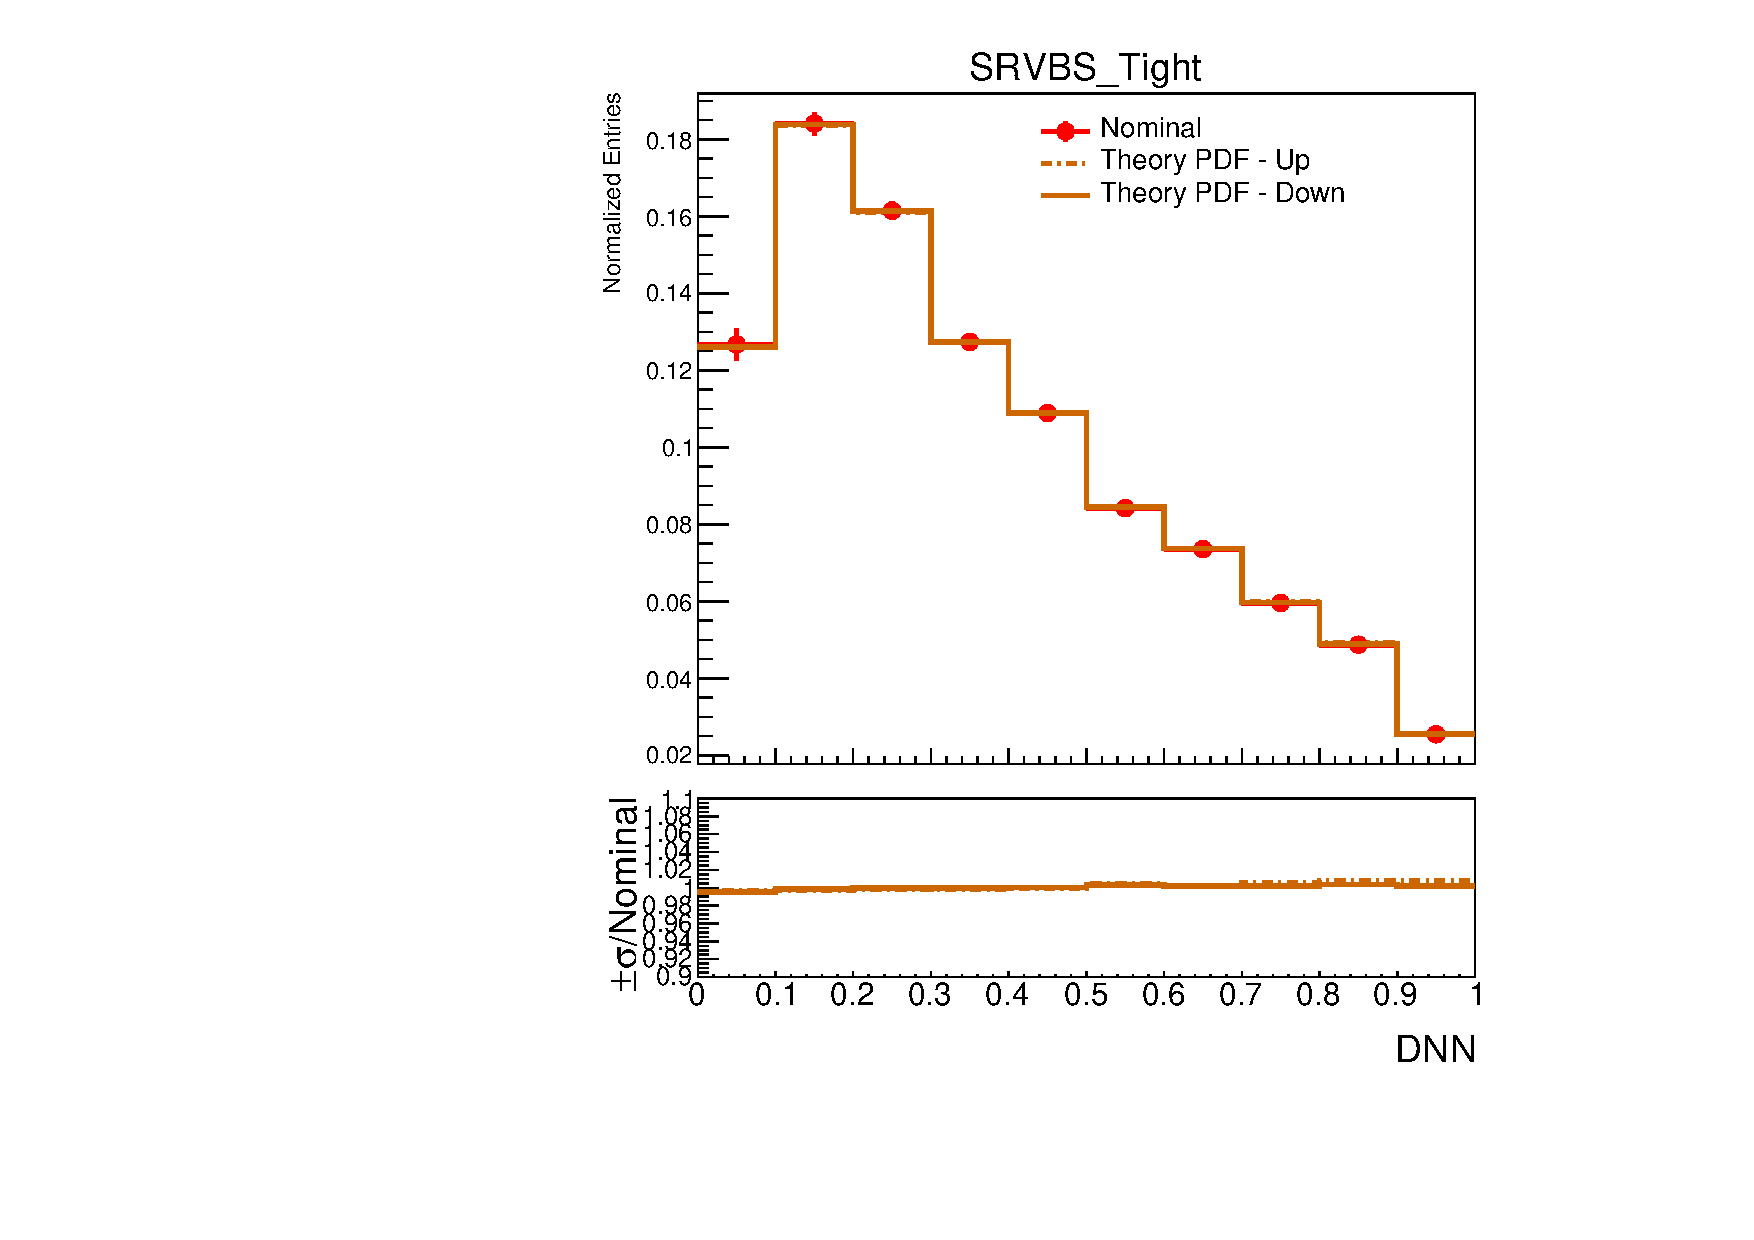
\includegraphics[width=\textwidth]{figures/1lep/PDFUnc/TheoryPDF/W_0ptag2pjet_0ptv_SRVBS_Tight_DNN_SysTheoryPDF_W__1up_Norm.pdf}
        \caption{\Wjets, resolved SR}
    \end{subfigure}
    \begin{subfigure}[b]{0.3\textwidth}
        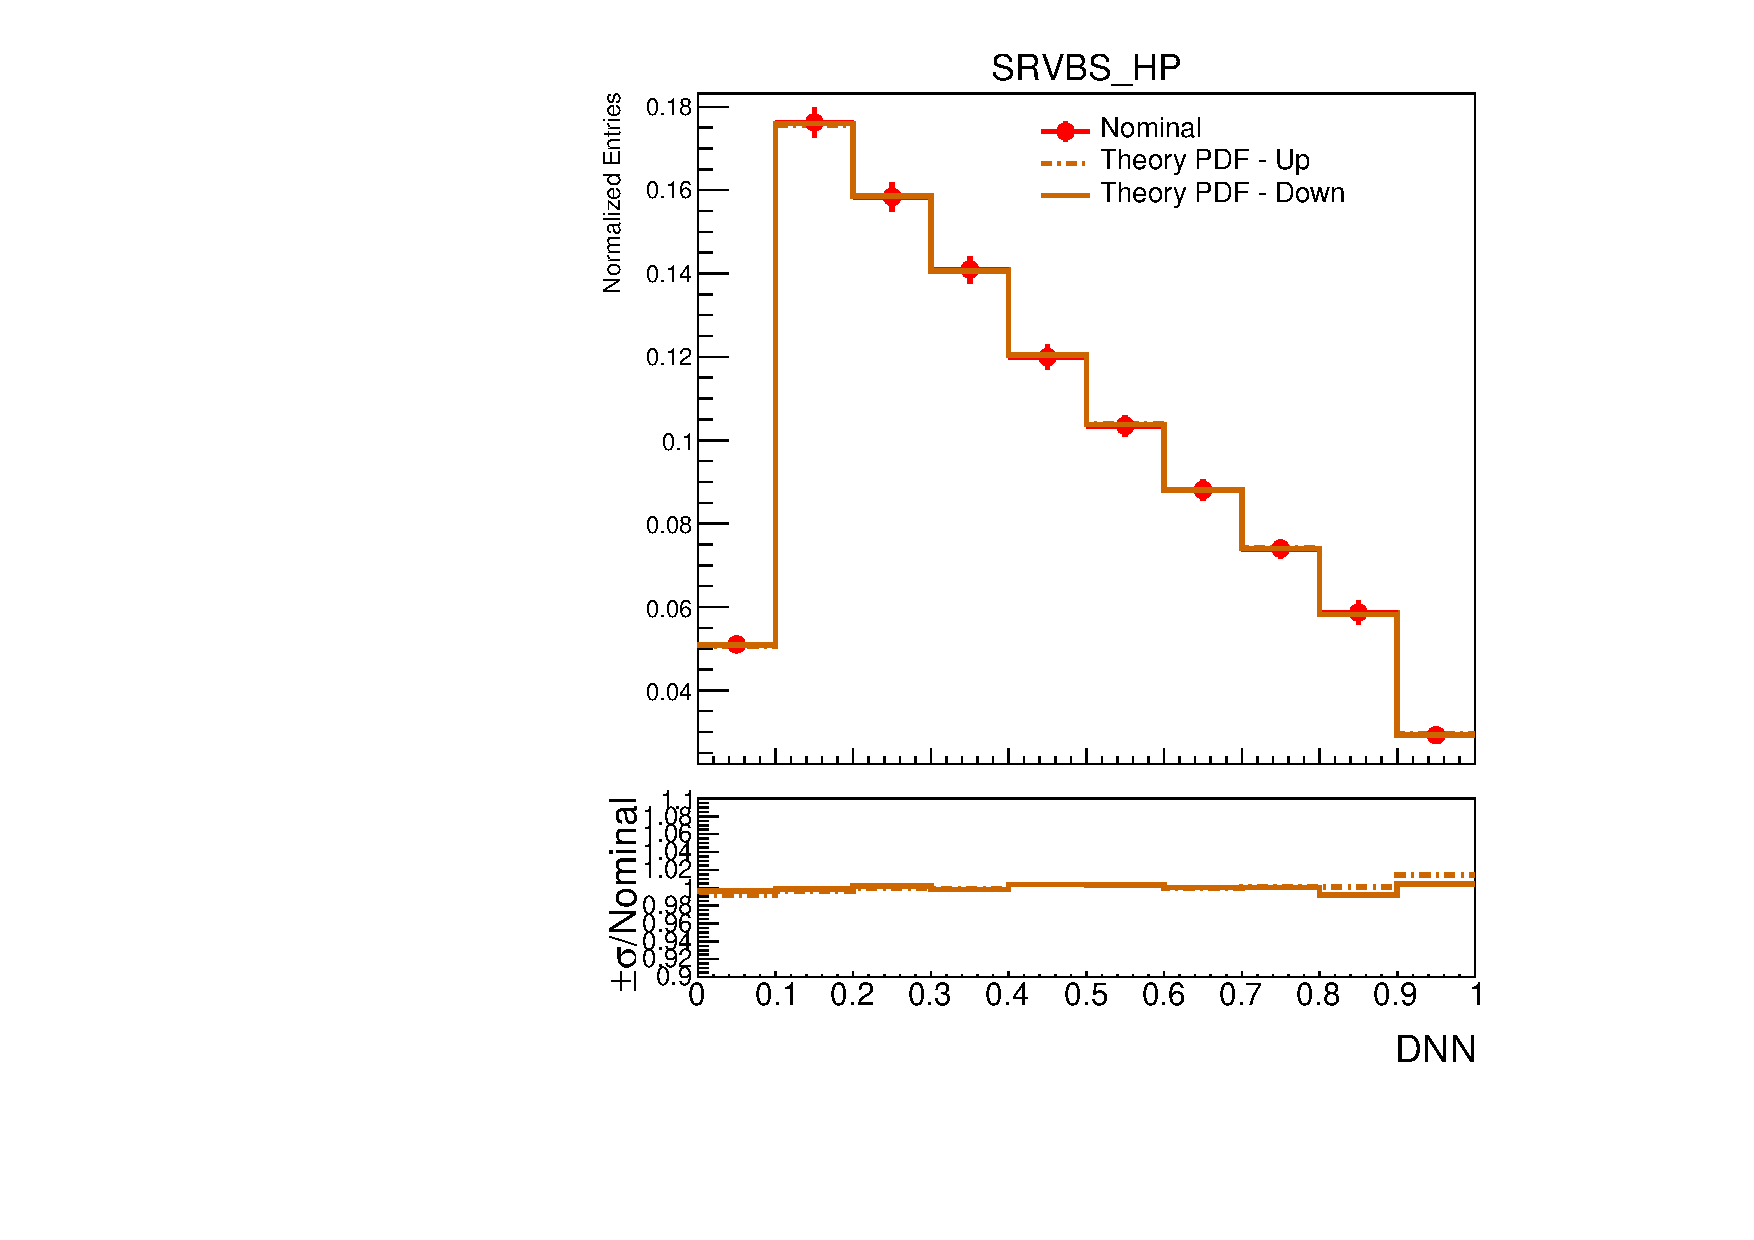
\includegraphics[width=\textwidth]{figures/1lep/PDFUnc/TheoryPDF/W_0ptag1pfat0pjet_0ptv_SRVBS_HP_DNN_SysTheoryPDF_W__1up_Norm.pdf}
        \caption{\Wjets, merged HP SR}
    \end{subfigure}
    \begin{subfigure}[b]{0.3\textwidth}
        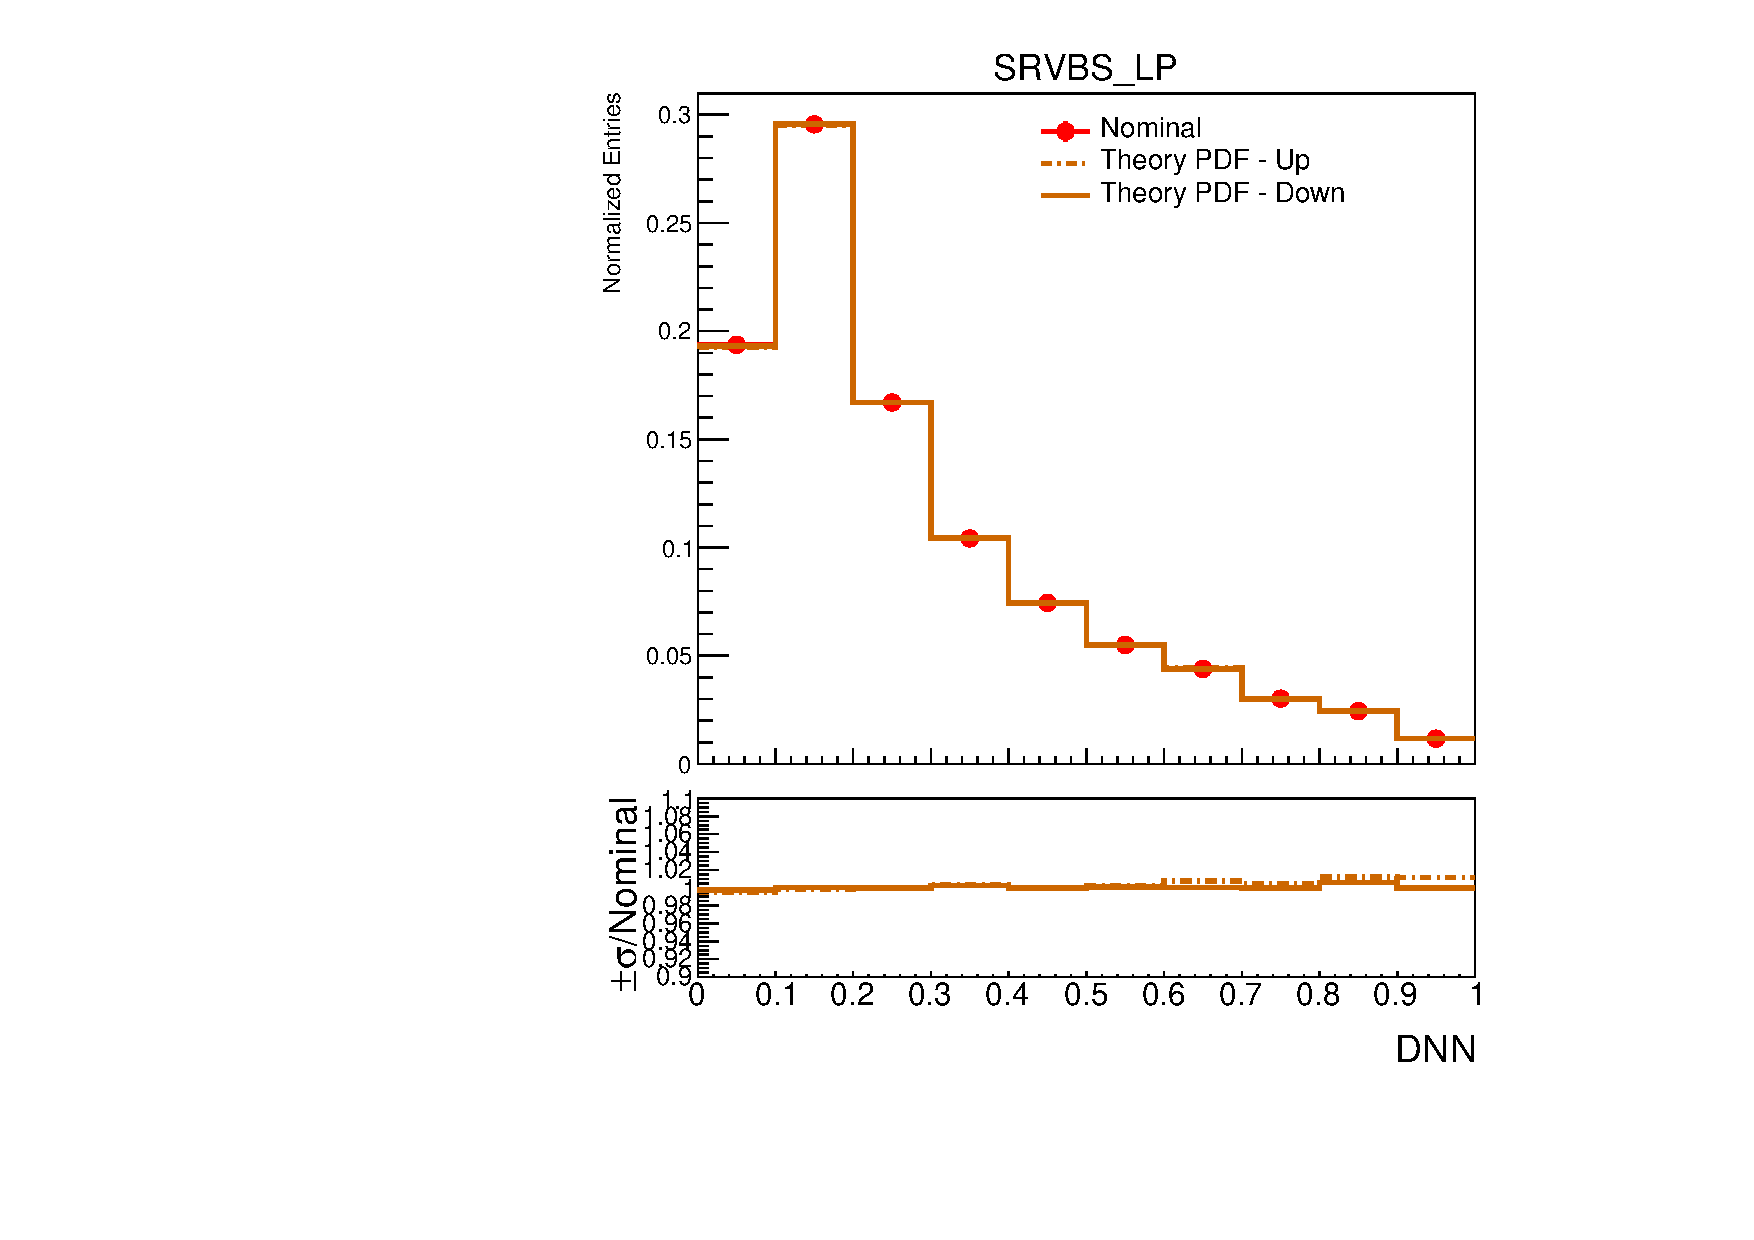
\includegraphics[width=\textwidth]{figures/1lep/PDFUnc/TheoryPDF/W_0ptag1pfat0pjet_0ptv_SRVBS_LP_DNN_SysTheoryPDF_W__1up_Norm.pdf}
        \caption{\Wjets, merged LP SR}
    \end{subfigure}
    \\
    \vspace{15mm}
    \begin{subfigure}[b]{0.3\textwidth}
        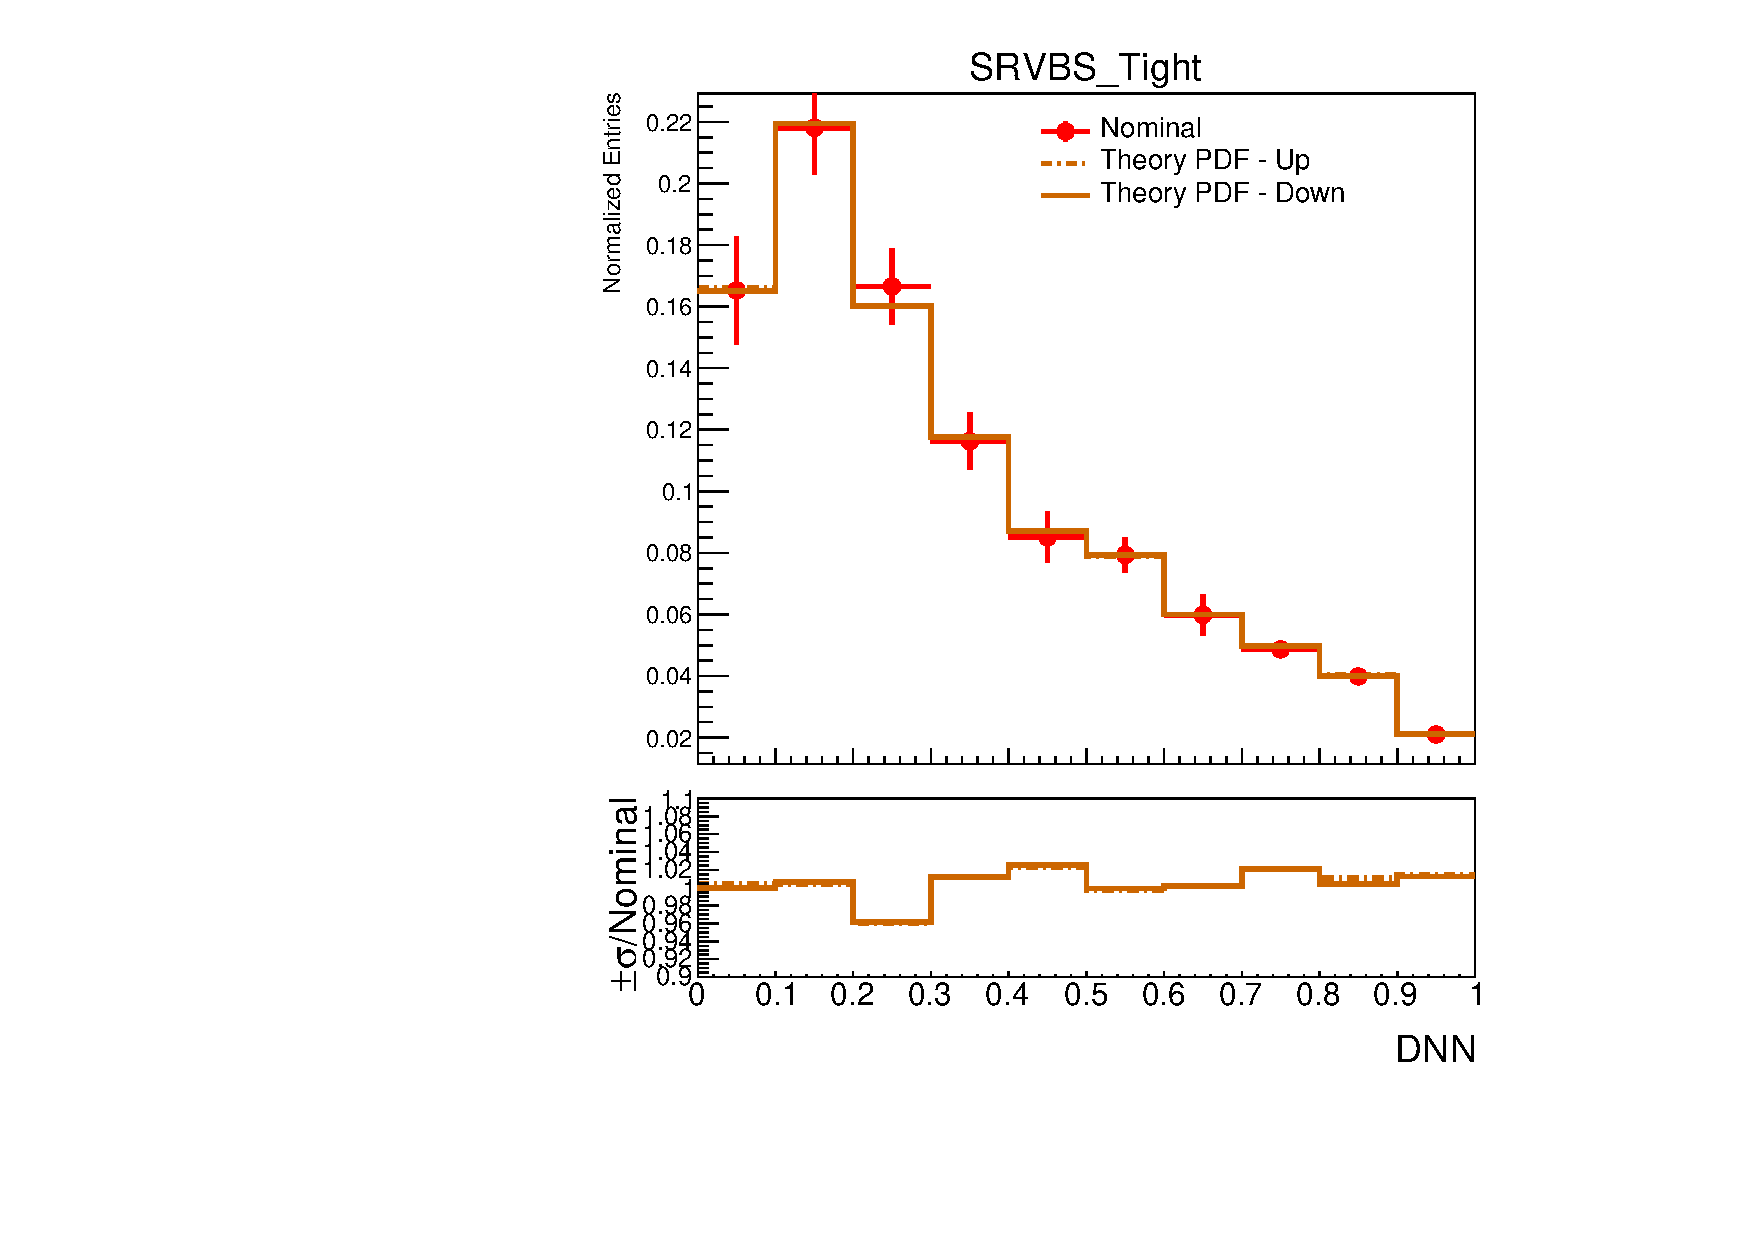
\includegraphics[width=\textwidth]{figures/1lep/PDFUnc/TheoryPDF/Z_0ptag2pjet_0ptv_SRVBS_Tight_DNN_SysTheoryPDF_Z__1up_Norm.pdf}
        \caption{\Zjets, resolved SR}
    \end{subfigure}
    \begin{subfigure}[b]{0.3\textwidth}
        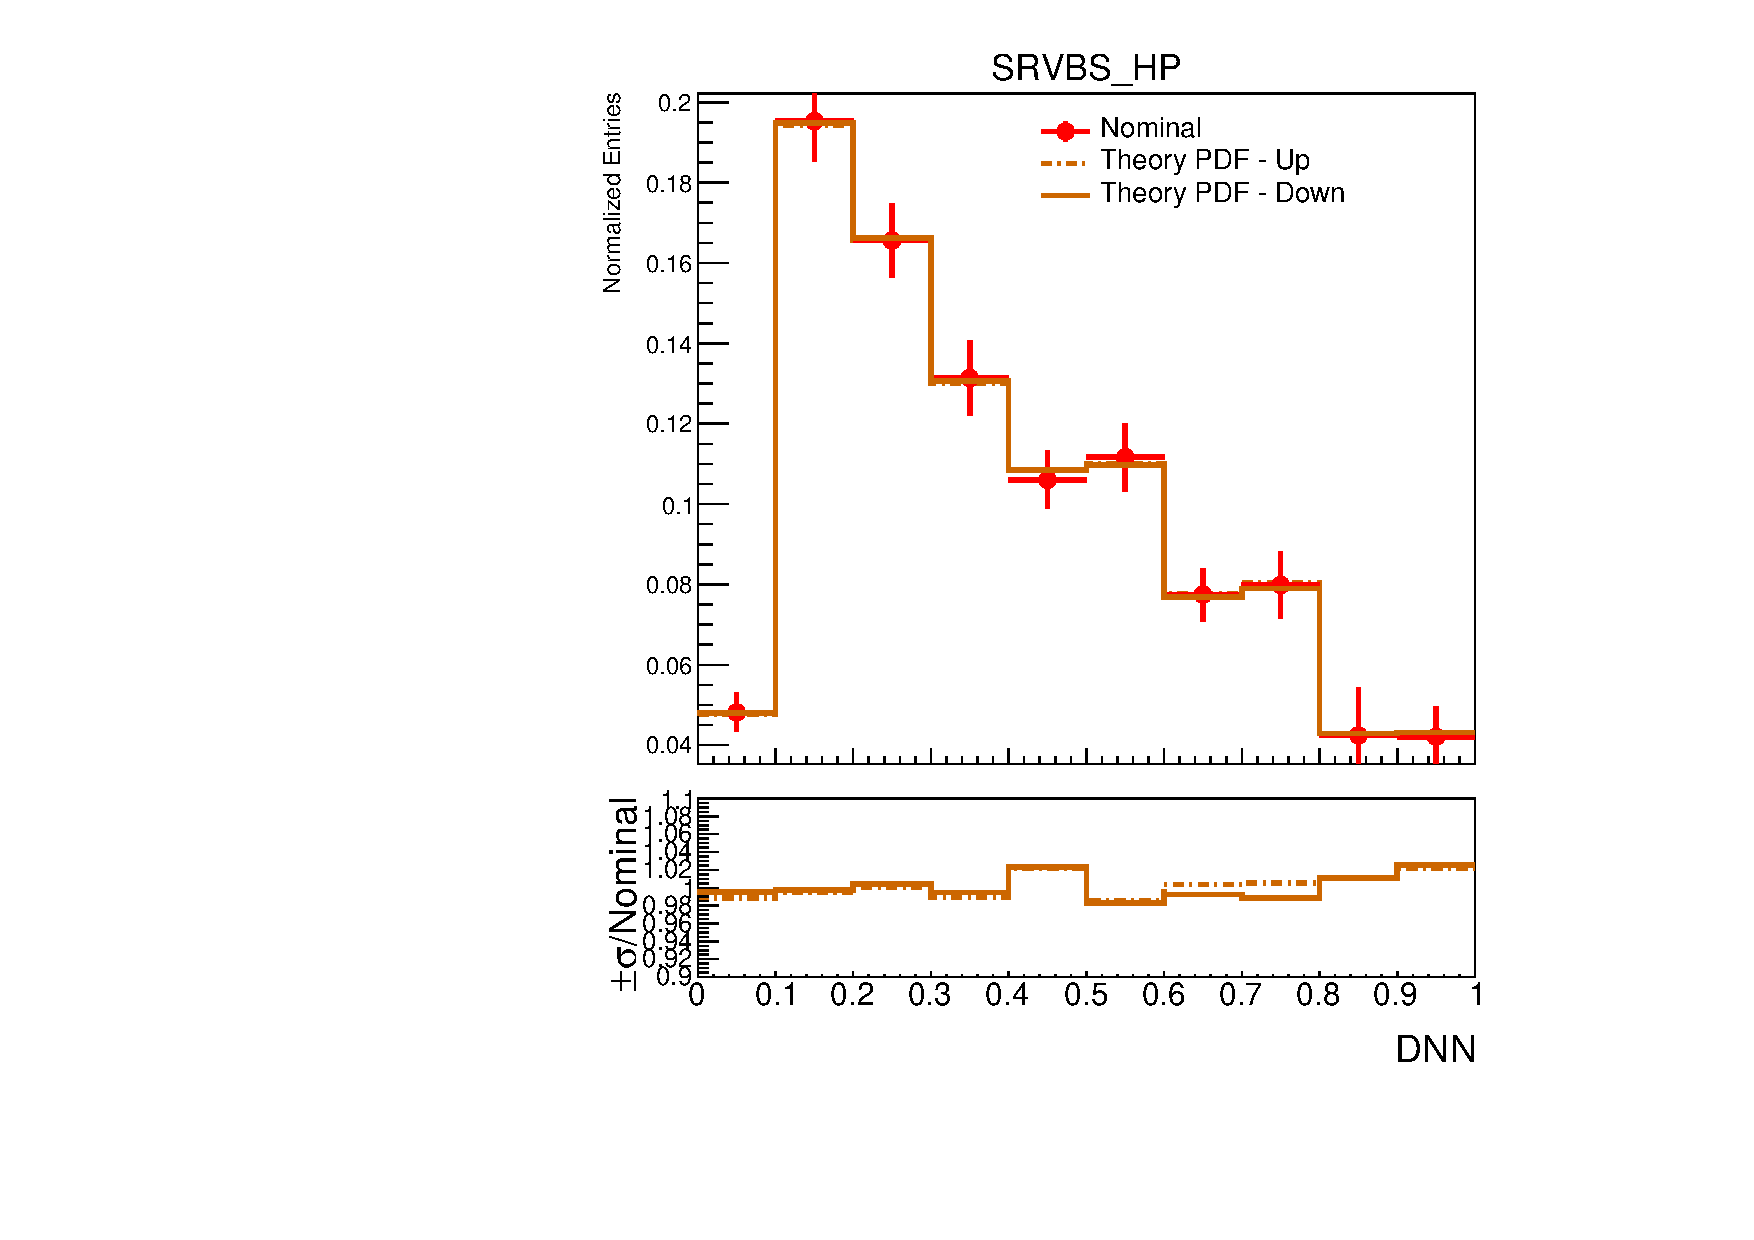
\includegraphics[width=\textwidth]{figures/1lep/PDFUnc/TheoryPDF/Z_0ptag1pfat0pjet_0ptv_SRVBS_HP_DNN_SysTheoryPDF_Z__1up_Norm.pdf}
        \caption{\Zjets, merged HP SR}
    \end{subfigure}
    \begin{subfigure}[b]{0.3\textwidth}
        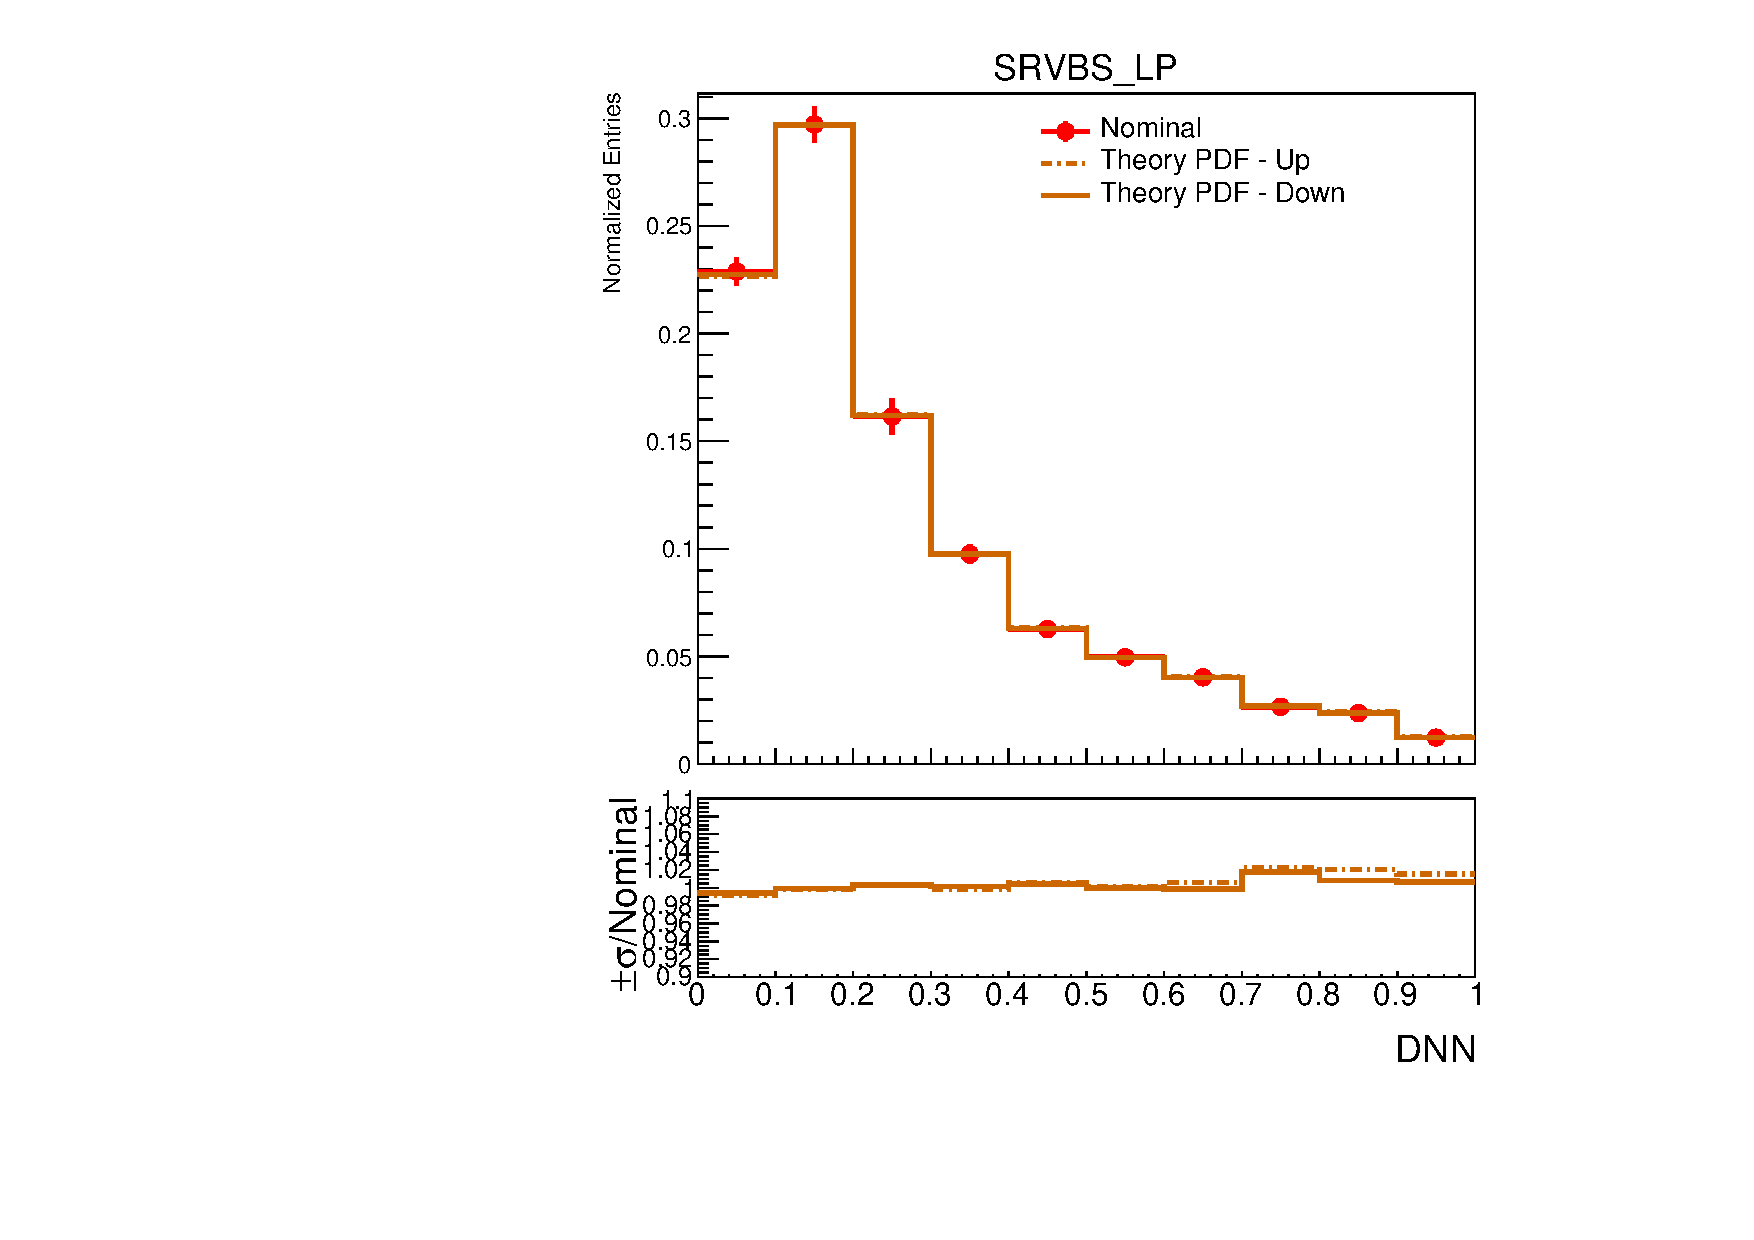
\includegraphics[width=\textwidth]{figures/1lep/PDFUnc/TheoryPDF/Z_0ptag1pfat0pjet_0ptv_SRVBS_LP_DNN_SysTheoryPDF_Z__1up_Norm.pdf}
        \caption{\Zjets, merged LP SR}
    \end{subfigure}
    \caption{Alternative PDF uncertainties in the 1-lepton channel. Histograms are normalized.}
    \label{fig:extPDFUnc1Lep}
\end{figure}


\begin{figure}[ht]
    \centering
    \begin{subfigure}[b]{0.3\textwidth}
        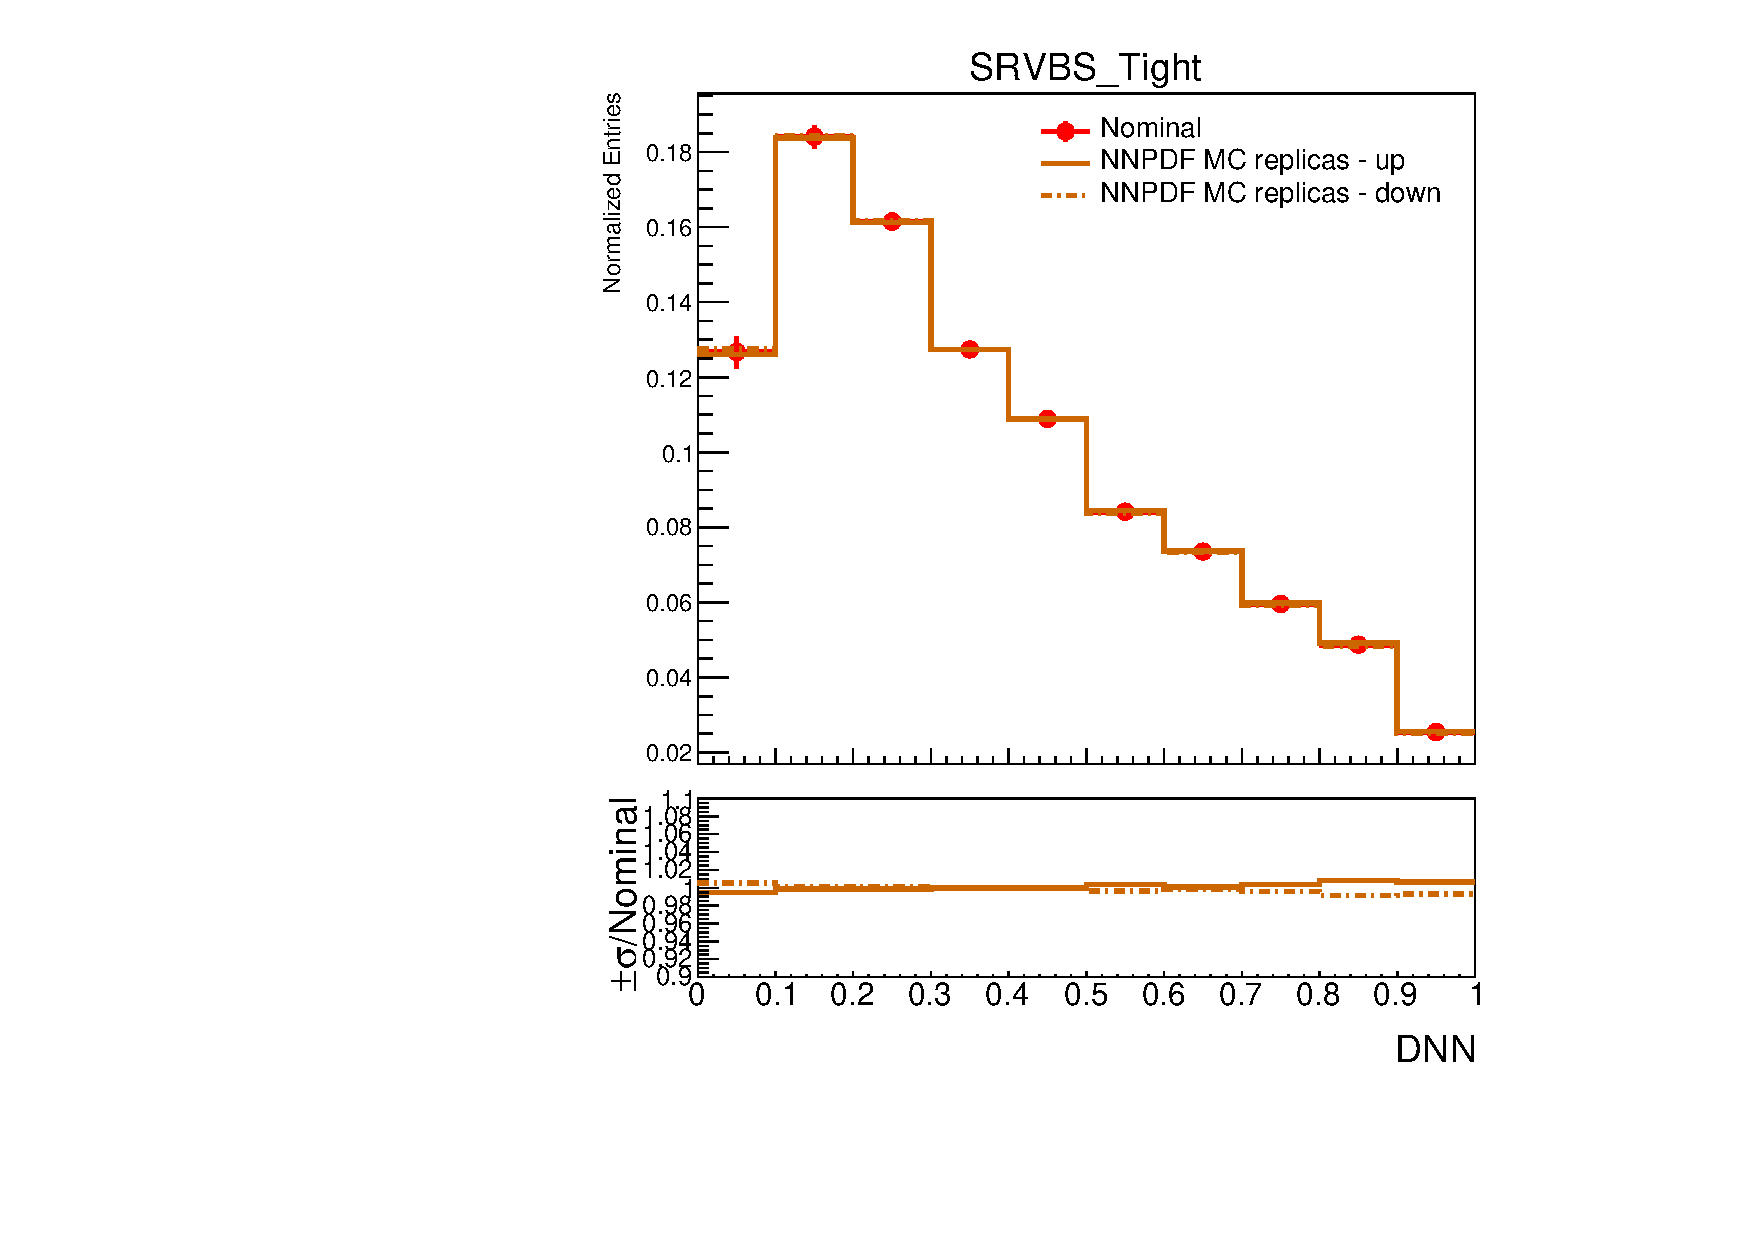
\includegraphics[width=\textwidth]{figures/1lep/PDFUnc/NNPDF/W_0ptag2pjet_0ptv_SRVBS_Tight_DNN_SysTheoryPDF_NNPDF_W__1up_Norm.pdf}
        \caption{\Wjets, resolved SR}
    \end{subfigure}
    \begin{subfigure}[b]{0.3\textwidth}
        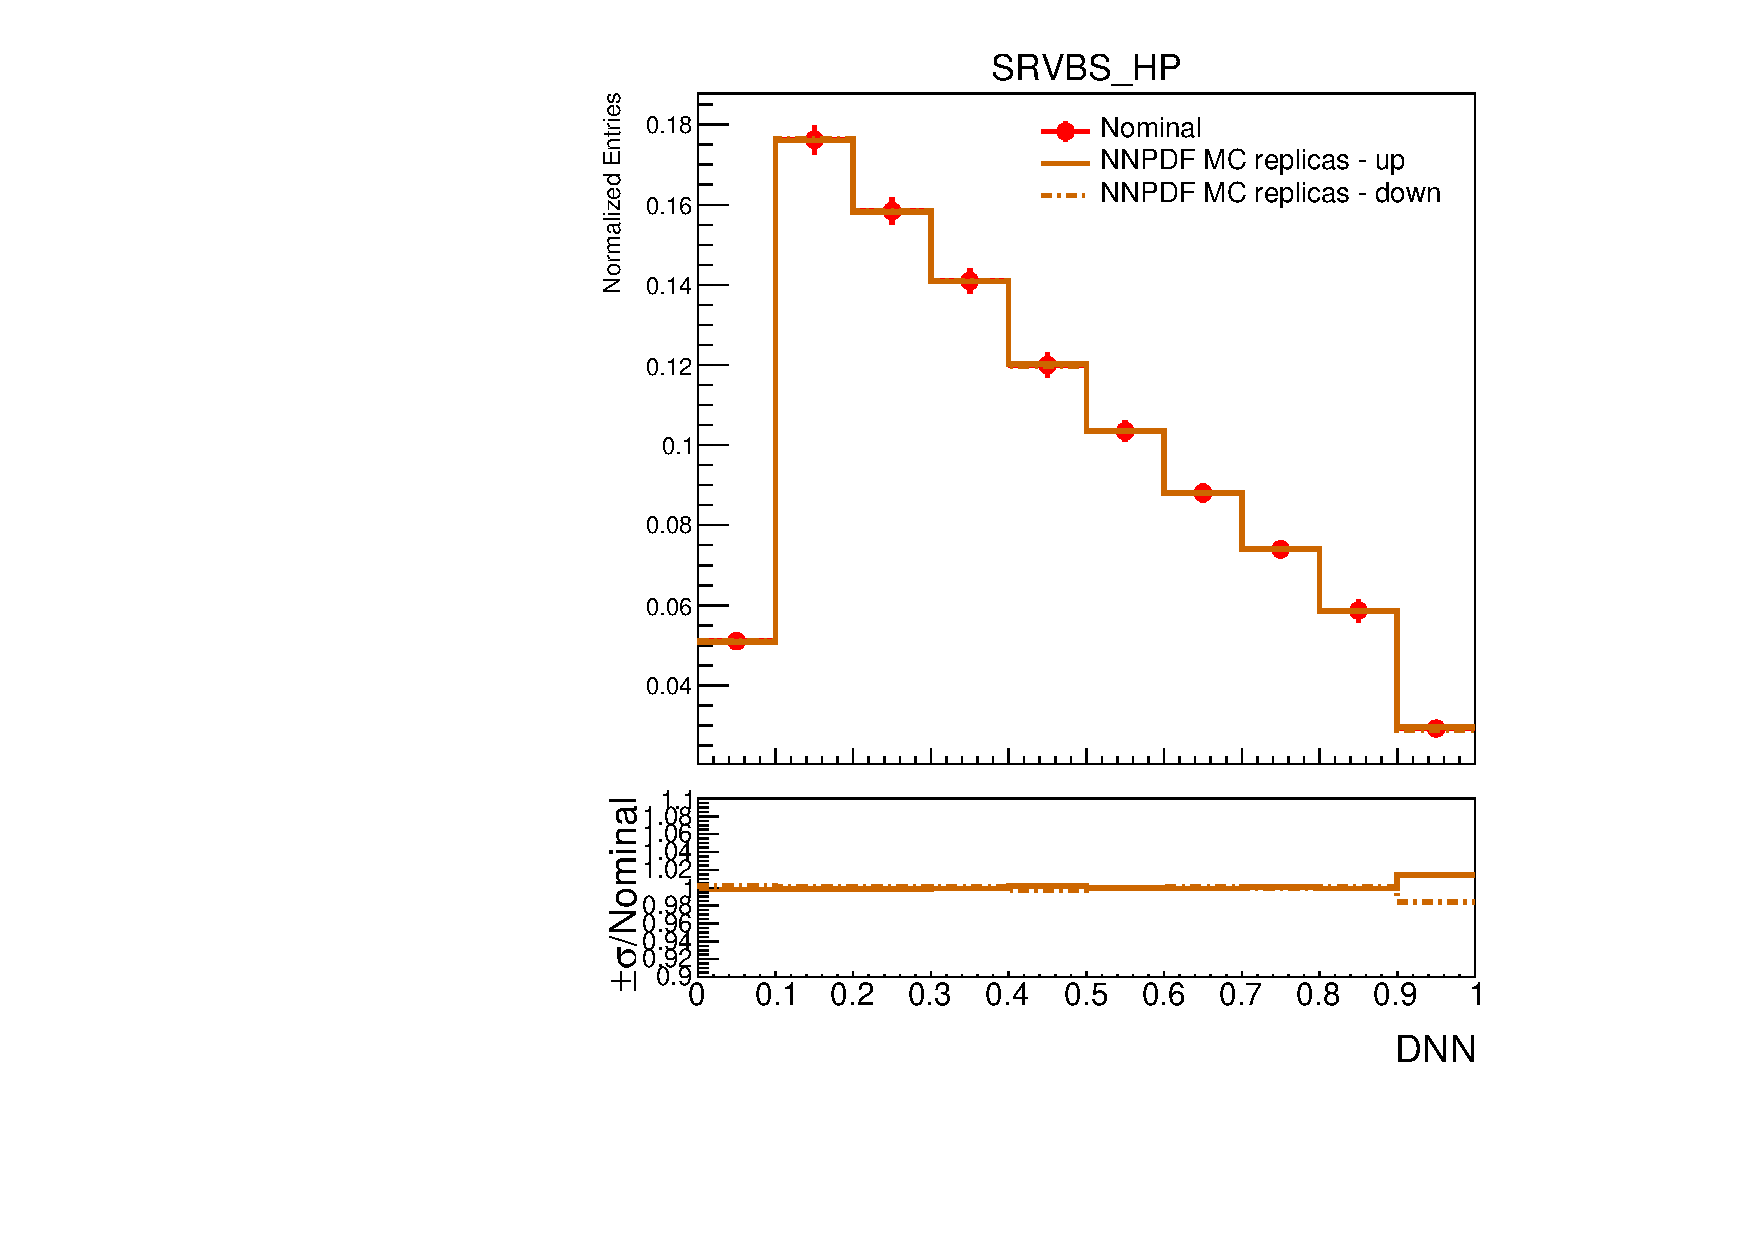
\includegraphics[width=\textwidth]{figures/1lep/PDFUnc/NNPDF/W_0ptag1pfat0pjet_0ptv_SRVBS_HP_DNN_SysTheoryPDF_NNPDF_W__1up_Norm.pdf}
        \caption{\Wjets, merged HP SR}
    \end{subfigure}
    \begin{subfigure}[b]{0.3\textwidth}
        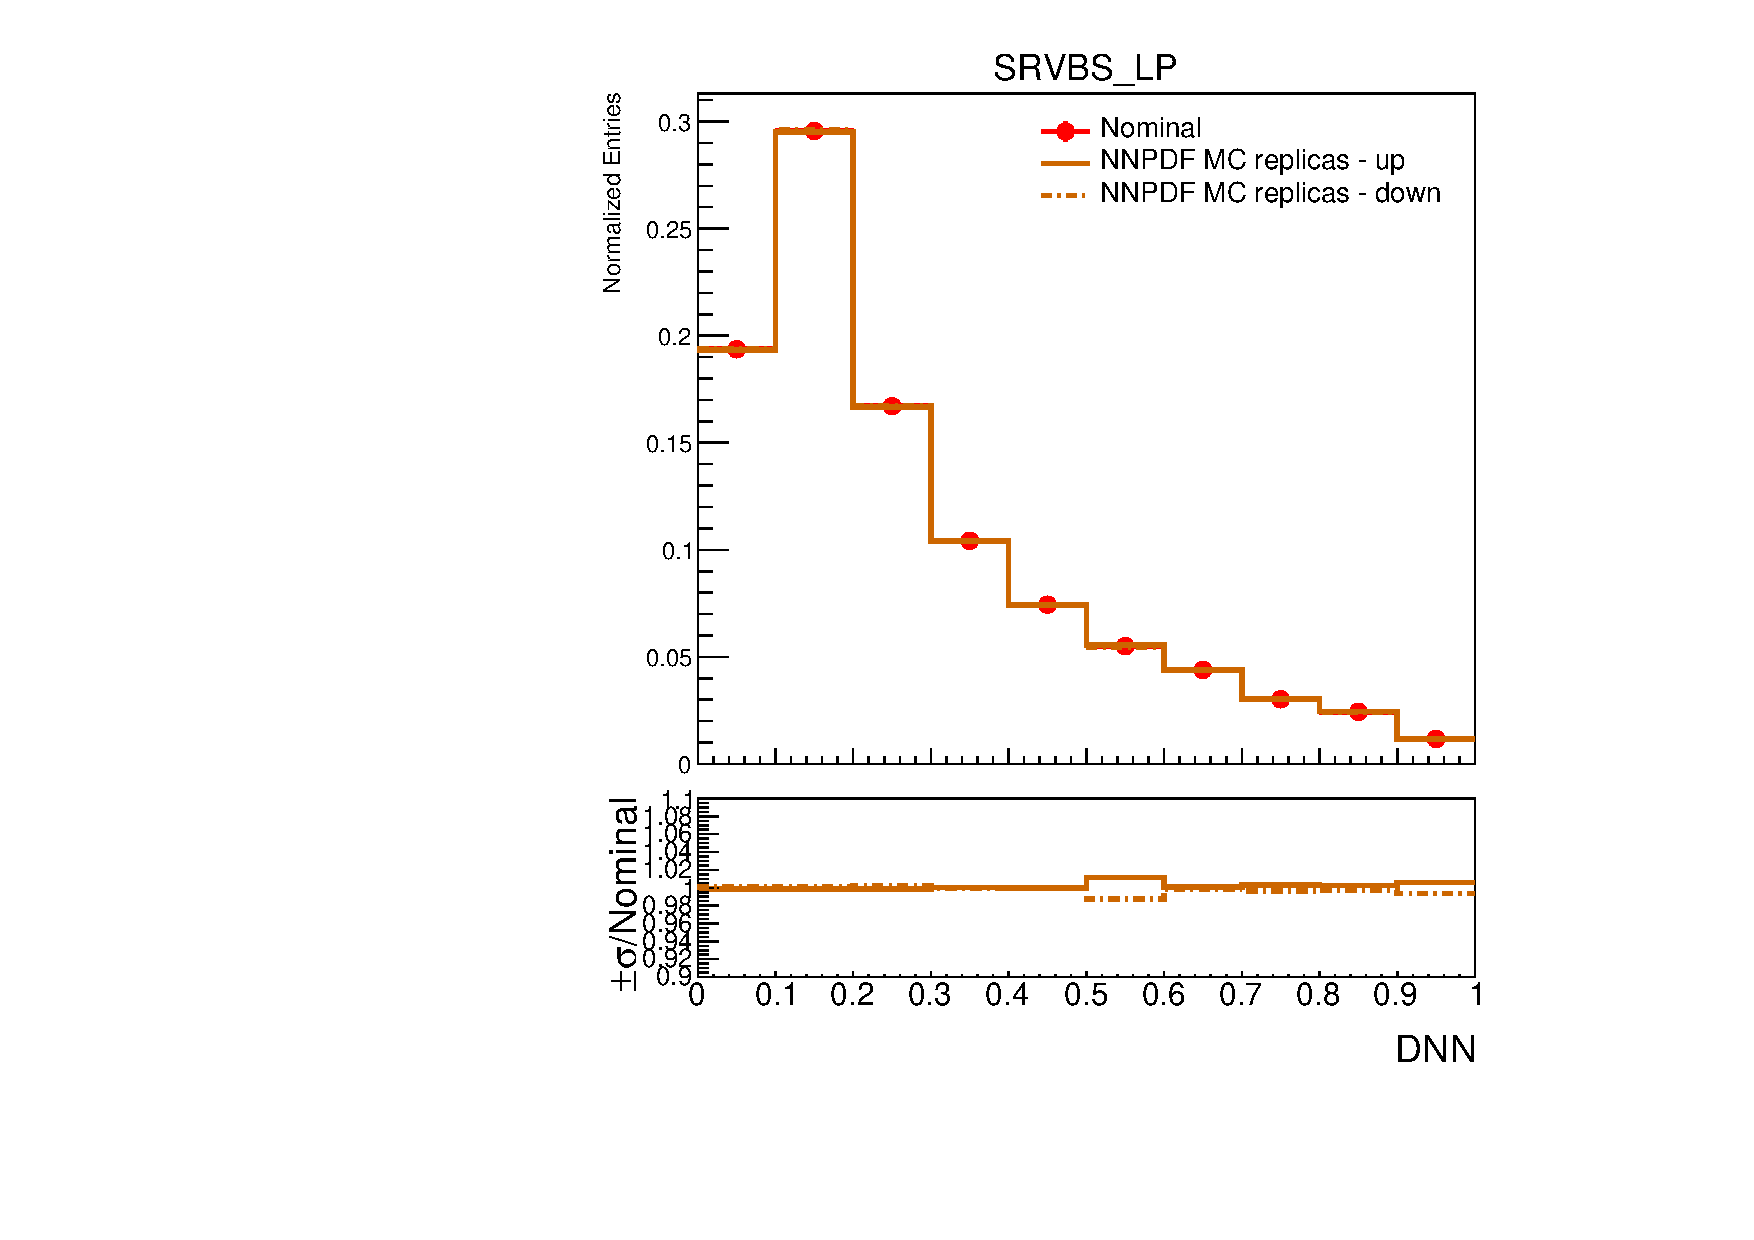
\includegraphics[width=\textwidth]{figures/1lep/PDFUnc/NNPDF/W_0ptag1pfat0pjet_0ptv_SRVBS_LP_DNN_SysTheoryPDF_NNPDF_W__1up_Norm.pdf}
        \caption{\Wjets, merged LP SR}
    \end{subfigure}
    \\
    \vspace{15mm}
    \begin{subfigure}[b]{0.3\textwidth}
        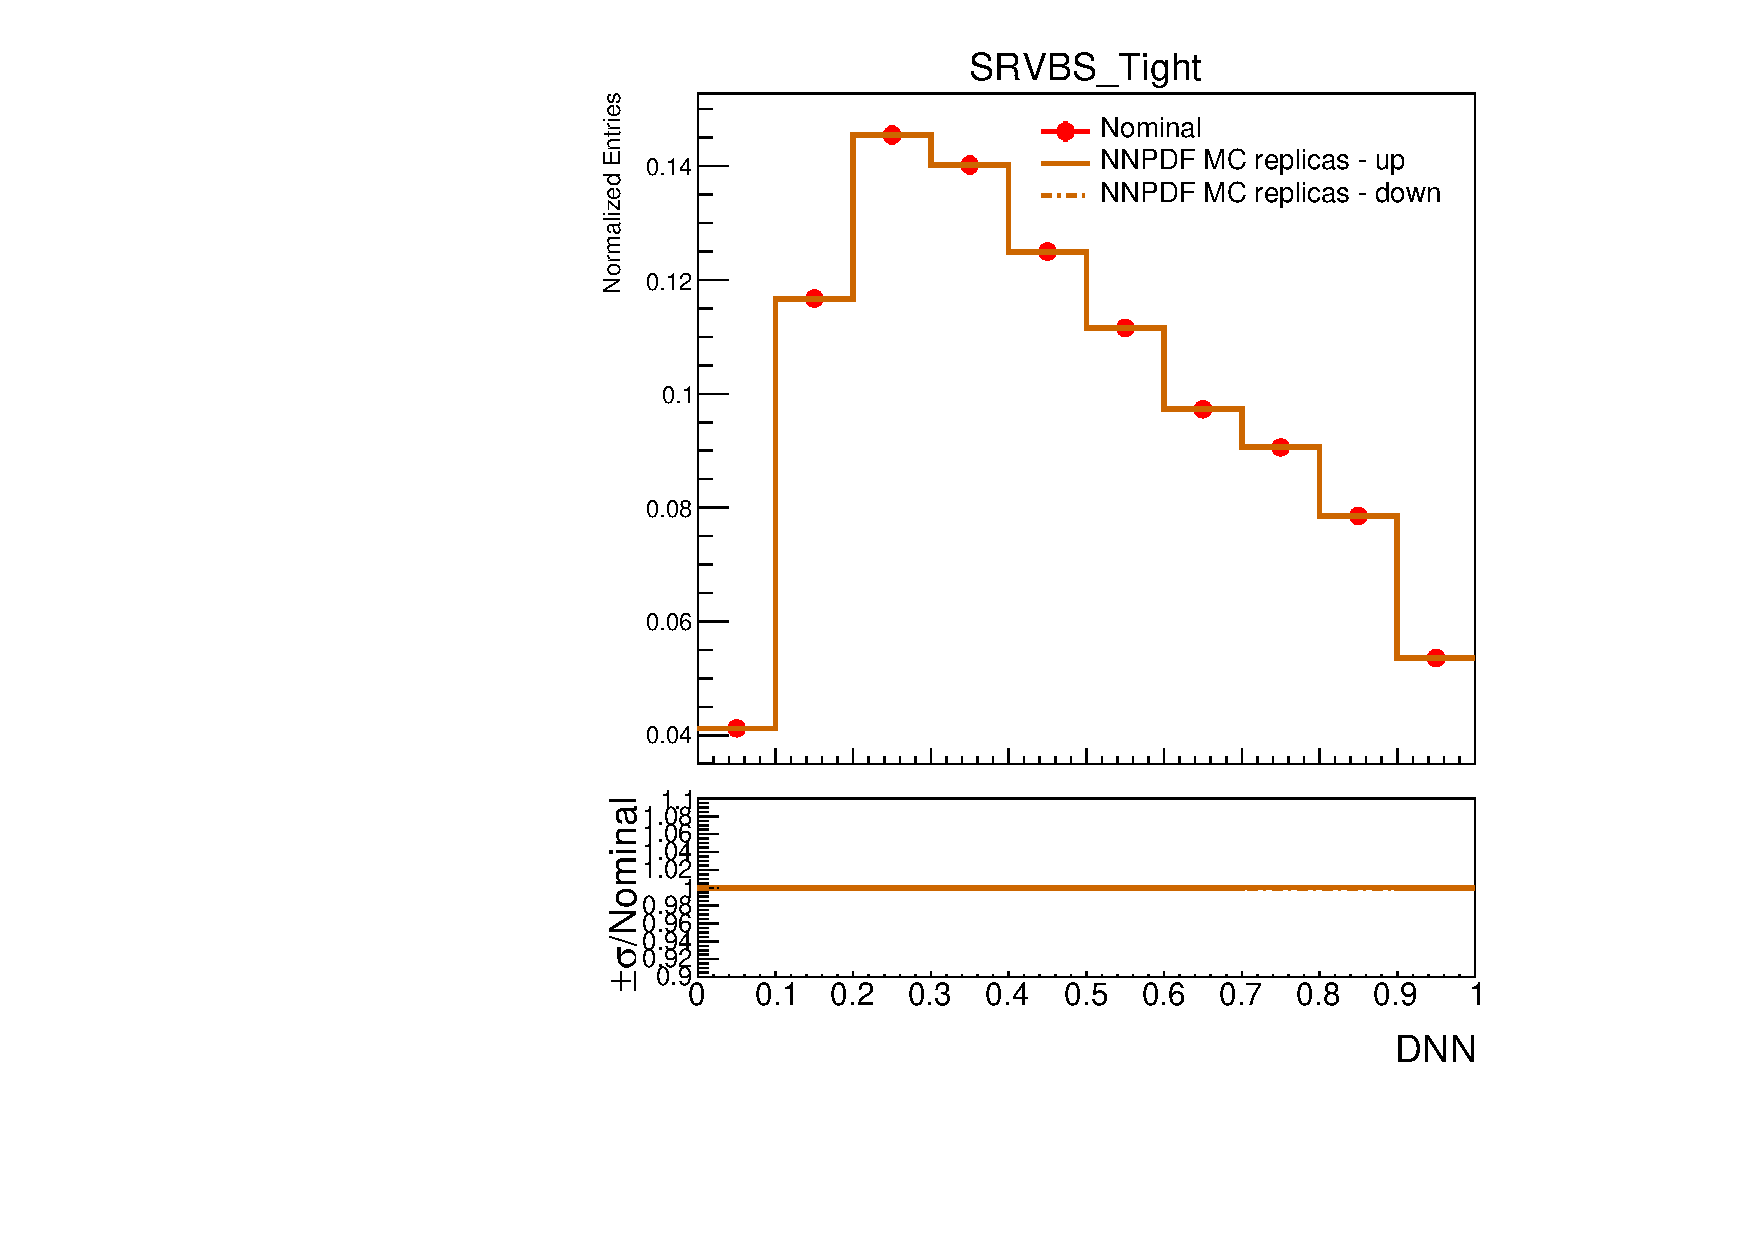
\includegraphics[width=\textwidth]{figures/1lep/PDFUnc/NNPDF/ttbar_0ptag2pjet_0ptv_SRVBS_Tight_DNN_SysTheoryPDF_NNPDF_ttbar__1up_Norm.pdf}
        \caption{\ttbar, resolved SR}
    \end{subfigure}
    \begin{subfigure}[b]{0.3\textwidth}
        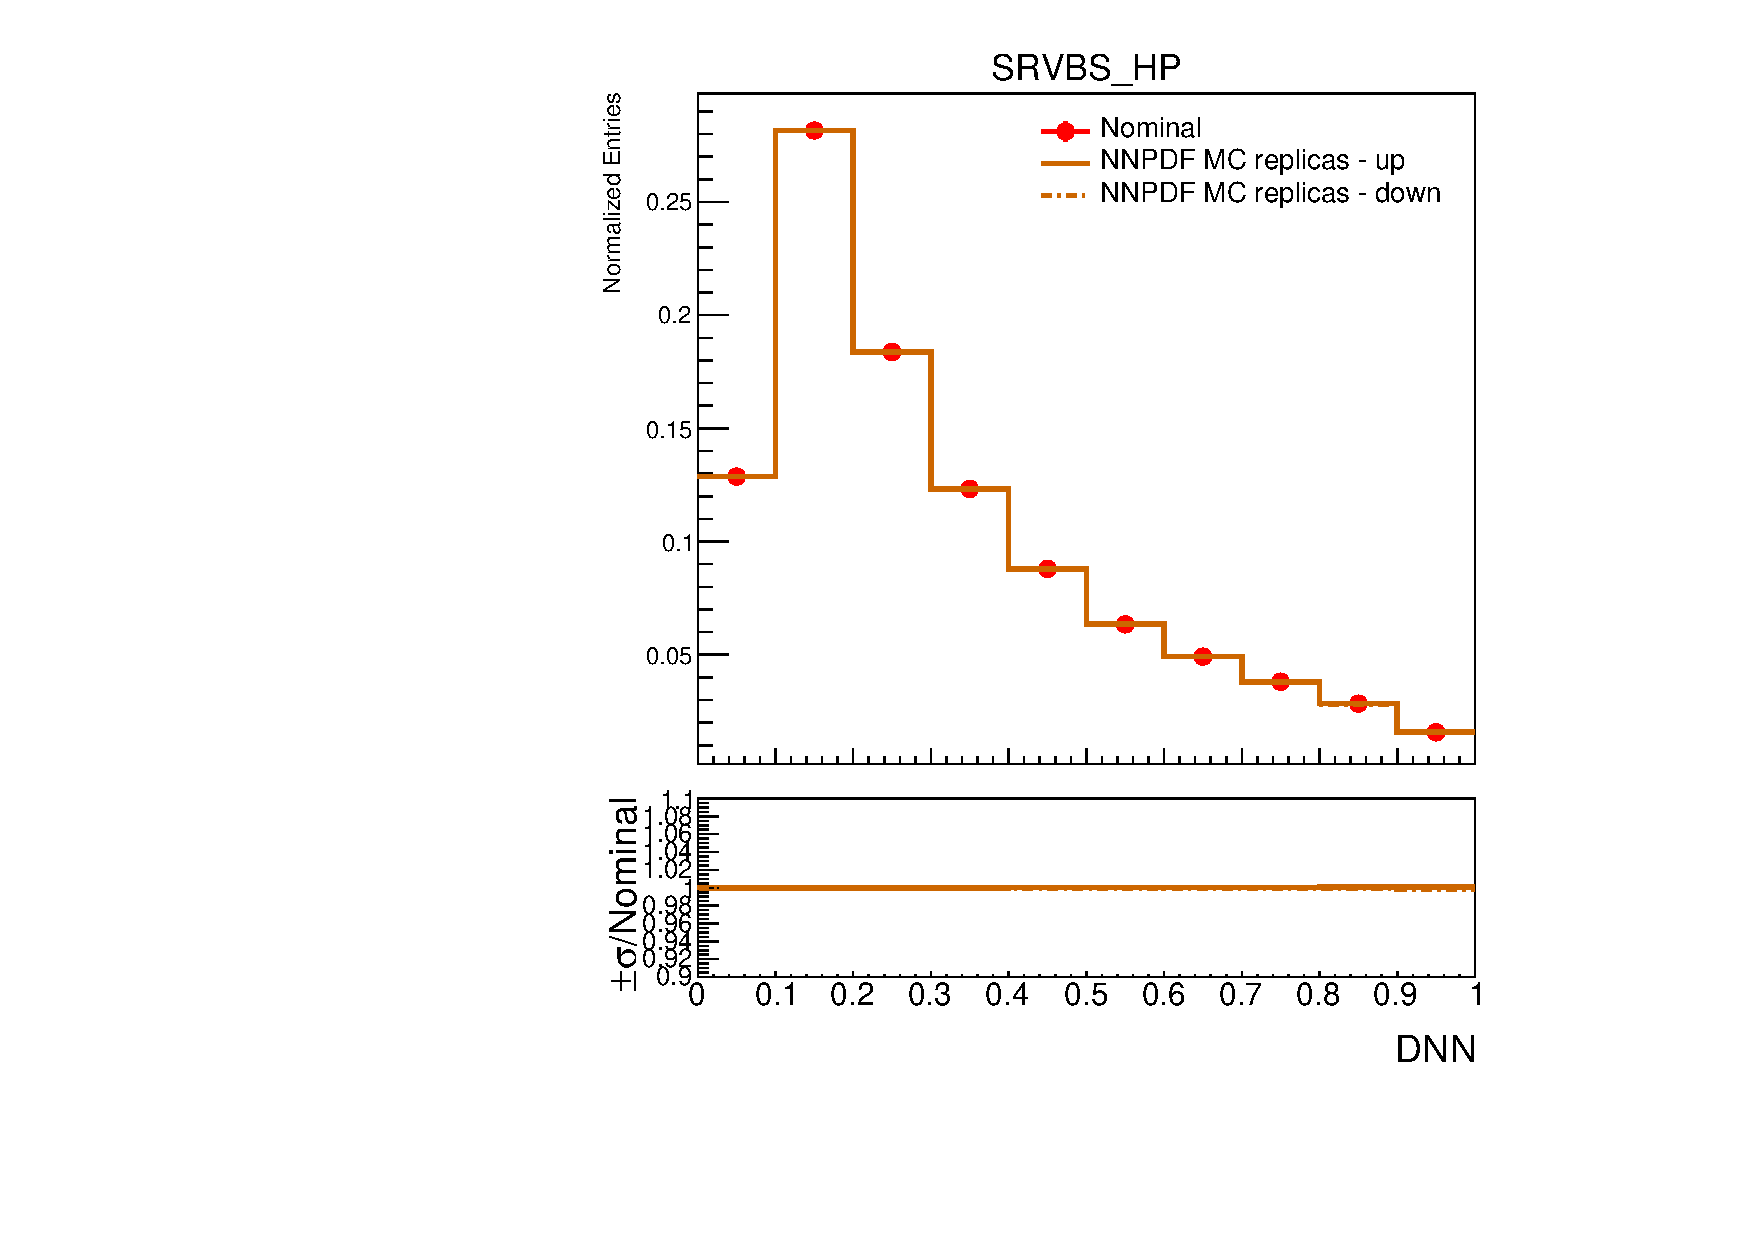
\includegraphics[width=\textwidth]{figures/1lep/PDFUnc/NNPDF/ttbar_0ptag1pfat0pjet_0ptv_SRVBS_HP_DNN_SysTheoryPDF_NNPDF_ttbar__1up_Norm.pdf}
        \caption{\ttbar, merged HP SR}
    \end{subfigure}
    \begin{subfigure}[b]{0.3\textwidth}
        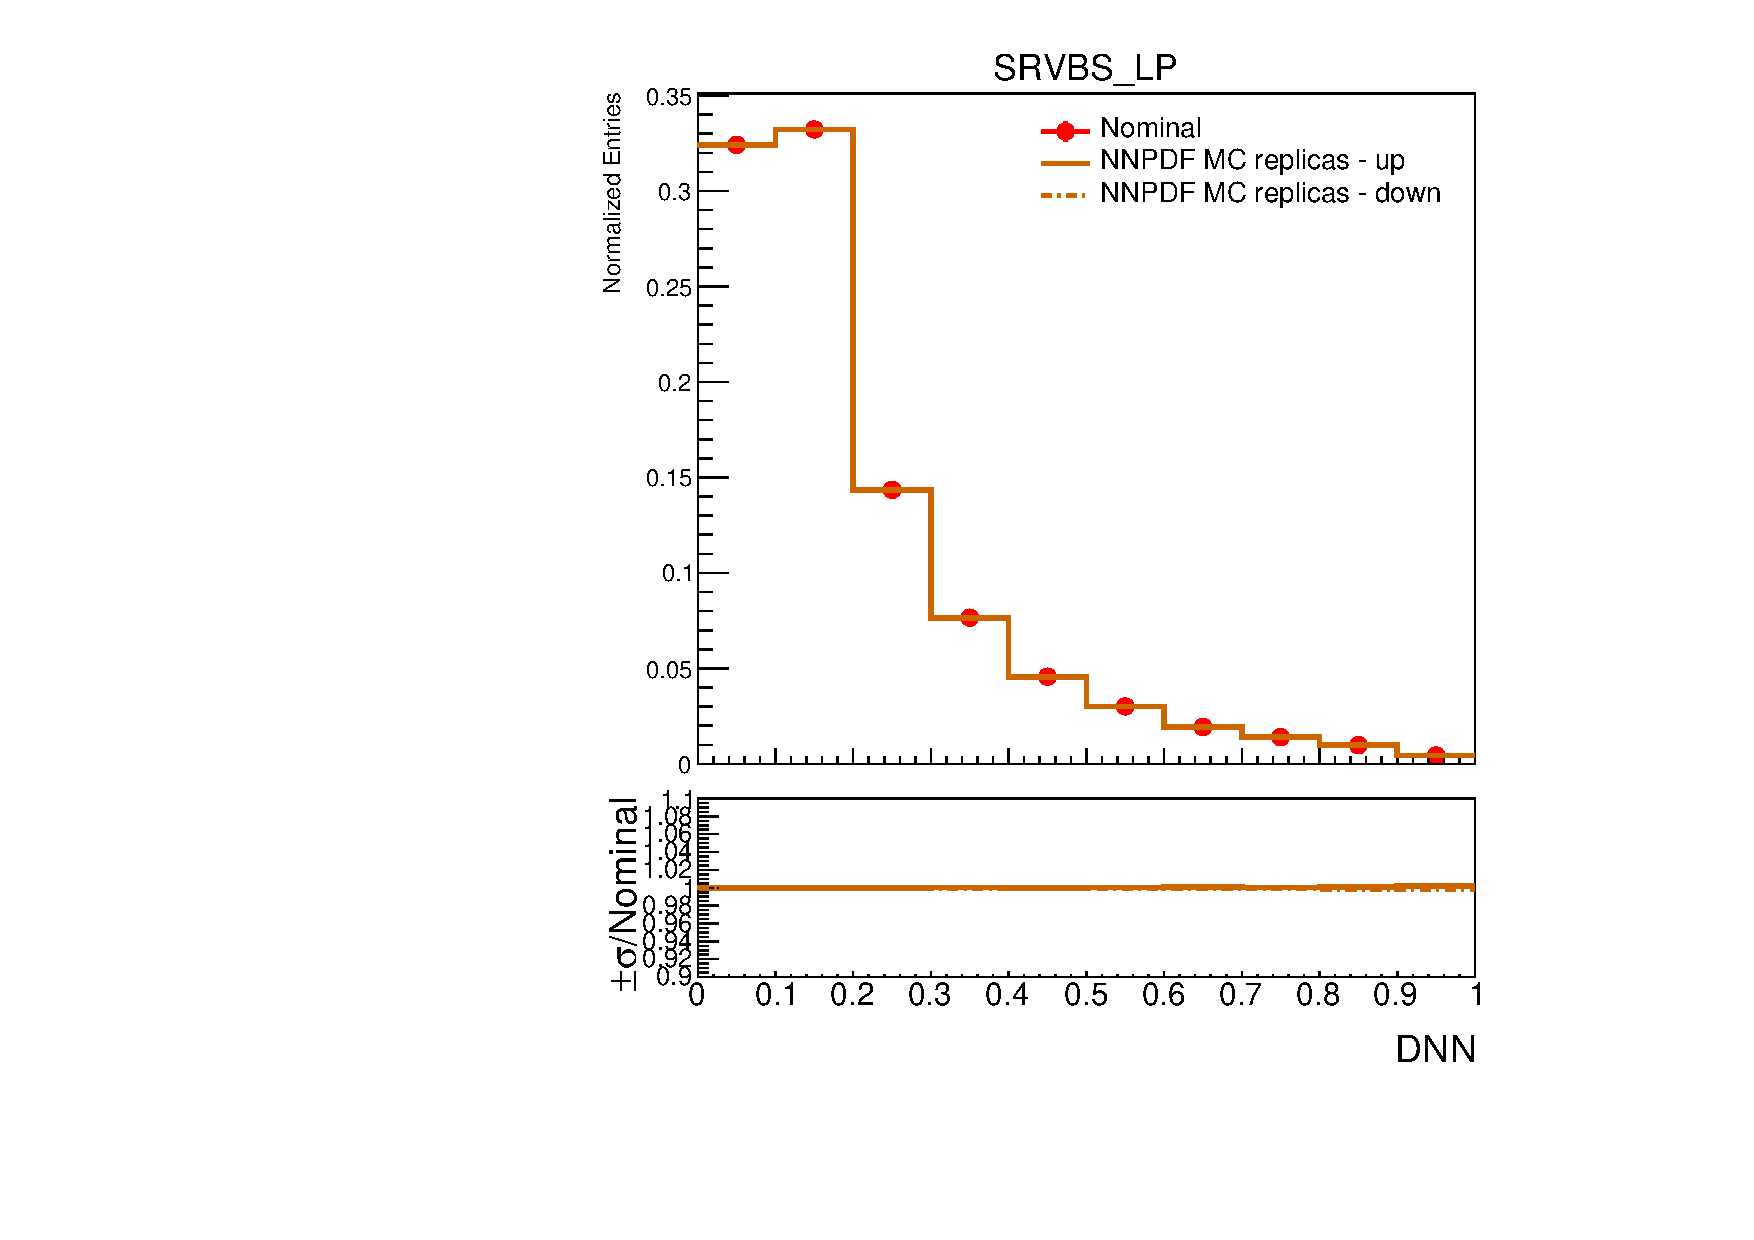
\includegraphics[width=\textwidth]{figures/1lep/PDFUnc/NNPDF/ttbar_0ptag1pfat0pjet_0ptv_SRVBS_LP_DNN_SysTheoryPDF_NNPDF_ttbar__1up_Norm.pdf}
        \caption{\ttbar, merged LP SR}
    \end{subfigure}
    \\
    \vspace{15mm}
    \begin{subfigure}[b]{0.3\textwidth}
        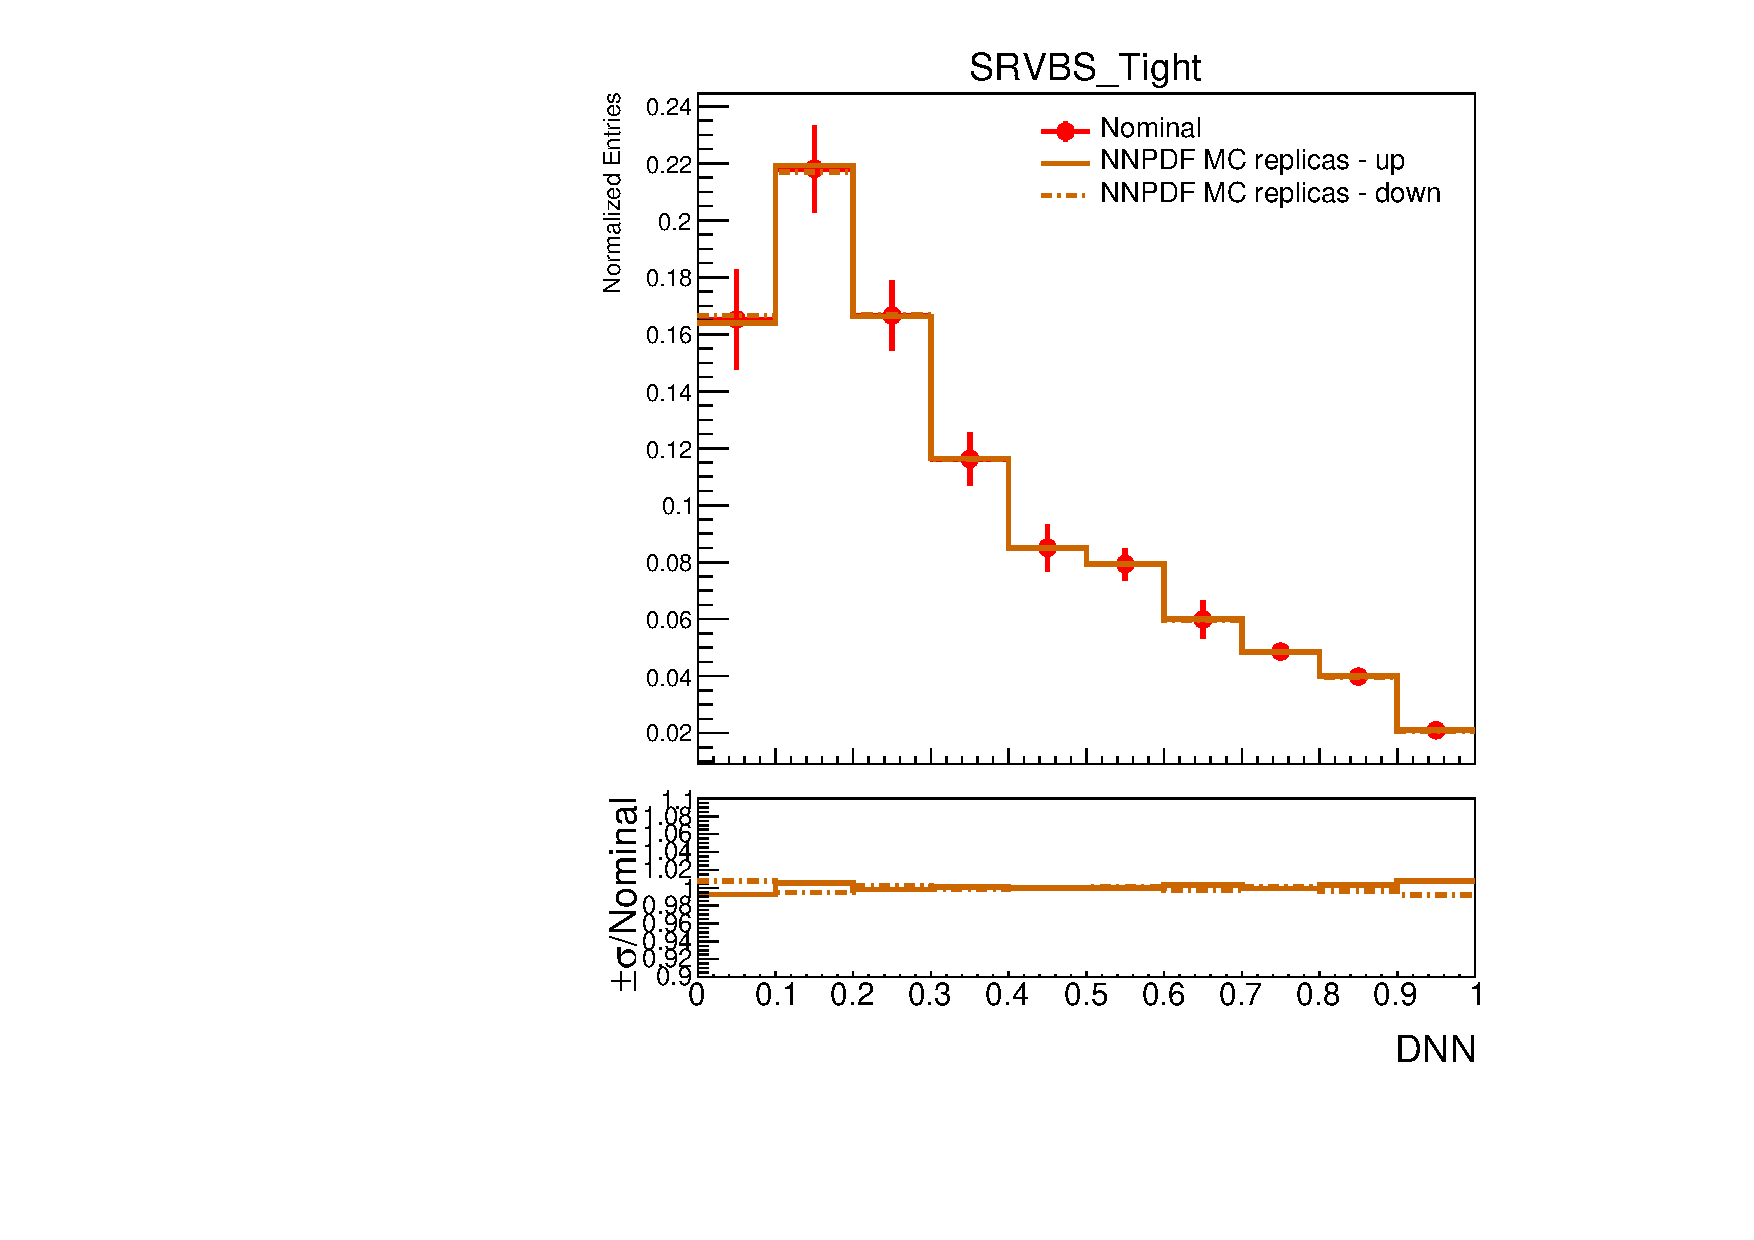
\includegraphics[width=\textwidth]{figures/1lep/PDFUnc/NNPDF/Z_0ptag2pjet_0ptv_SRVBS_Tight_DNN_SysTheoryPDF_NNPDF_Z__1up_Norm.pdf}
        \caption{\Zjets, resolved SR}
    \end{subfigure}
    \begin{subfigure}[b]{0.3\textwidth}
        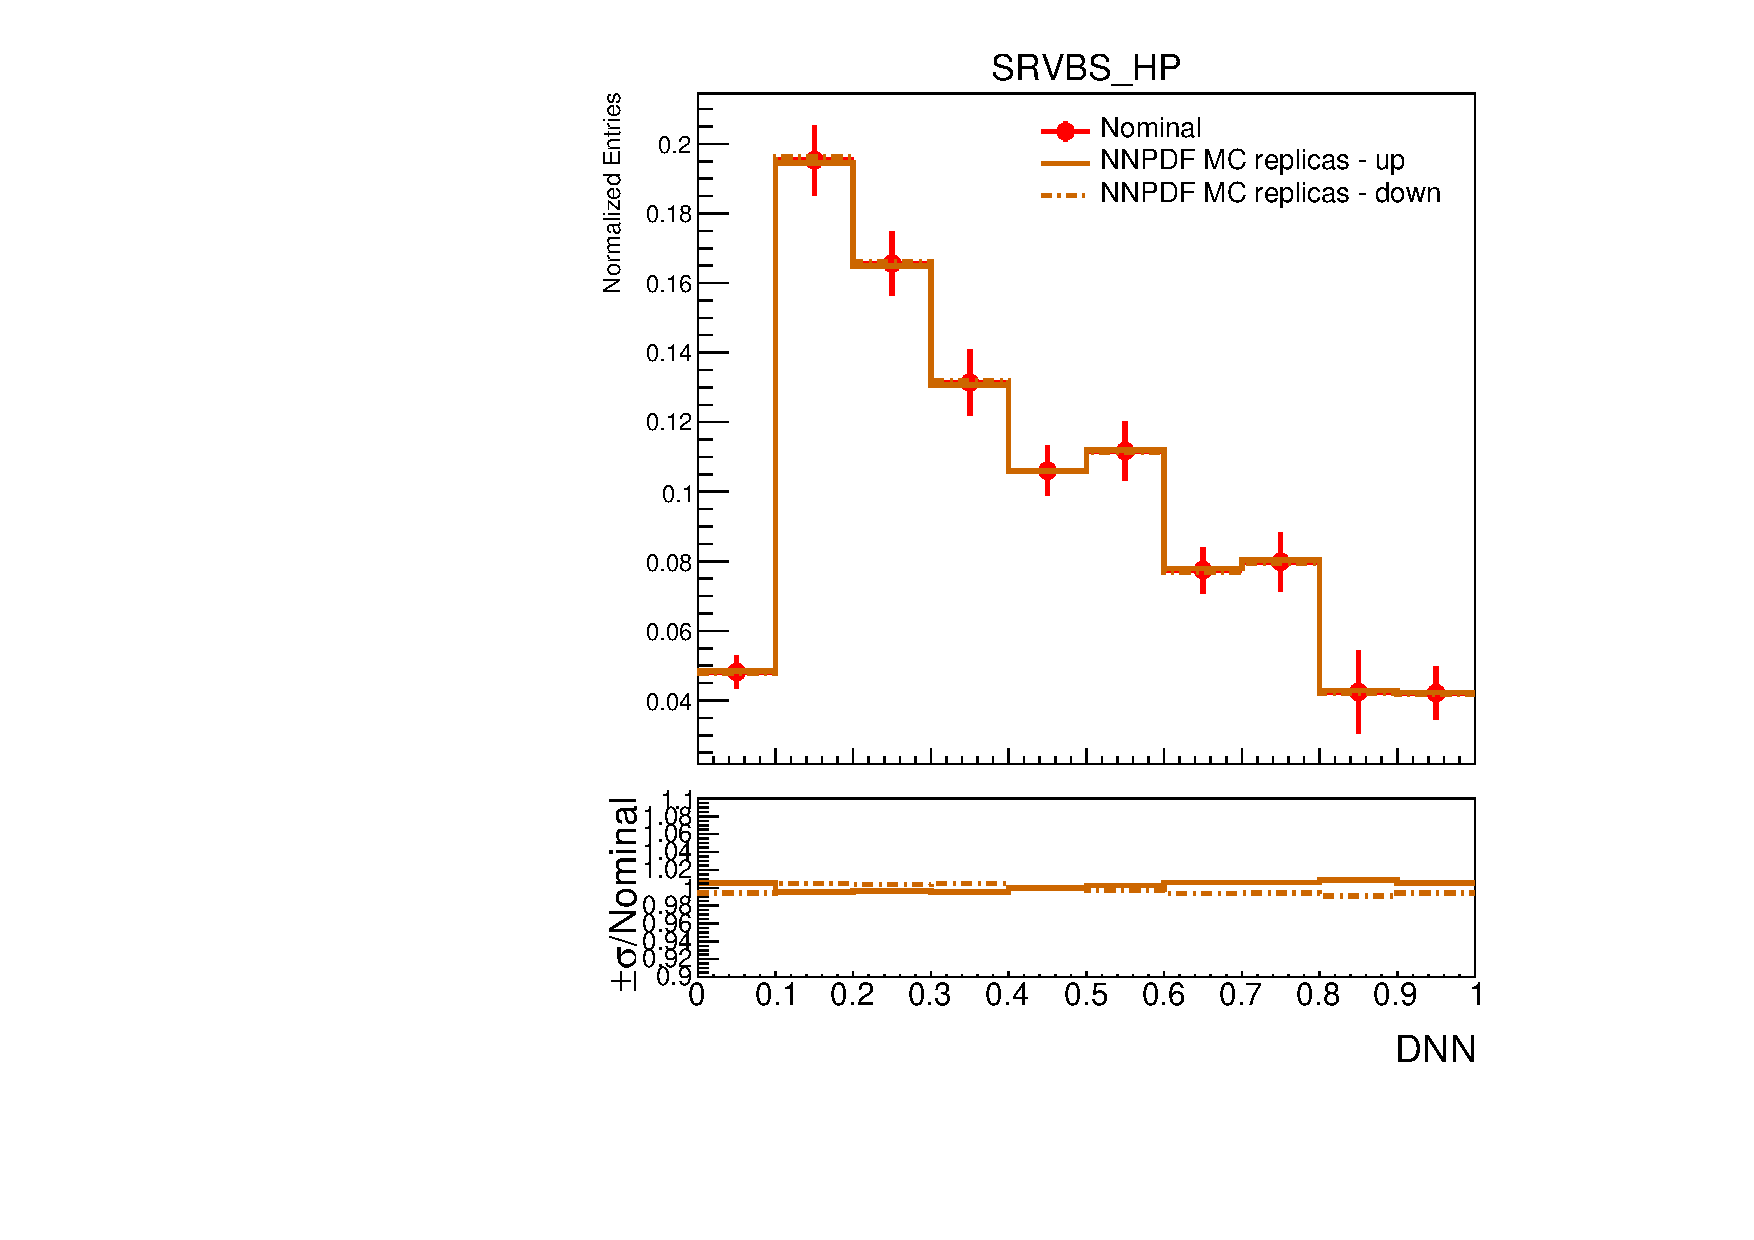
\includegraphics[width=\textwidth]{figures/1lep/PDFUnc/NNPDF/Z_0ptag1pfat0pjet_0ptv_SRVBS_HP_DNN_SysTheoryPDF_NNPDF_Z__1up_Norm.pdf}
        \caption{\Zjets, merged HP SR}
    \end{subfigure}
    \begin{subfigure}[b]{0.3\textwidth}
        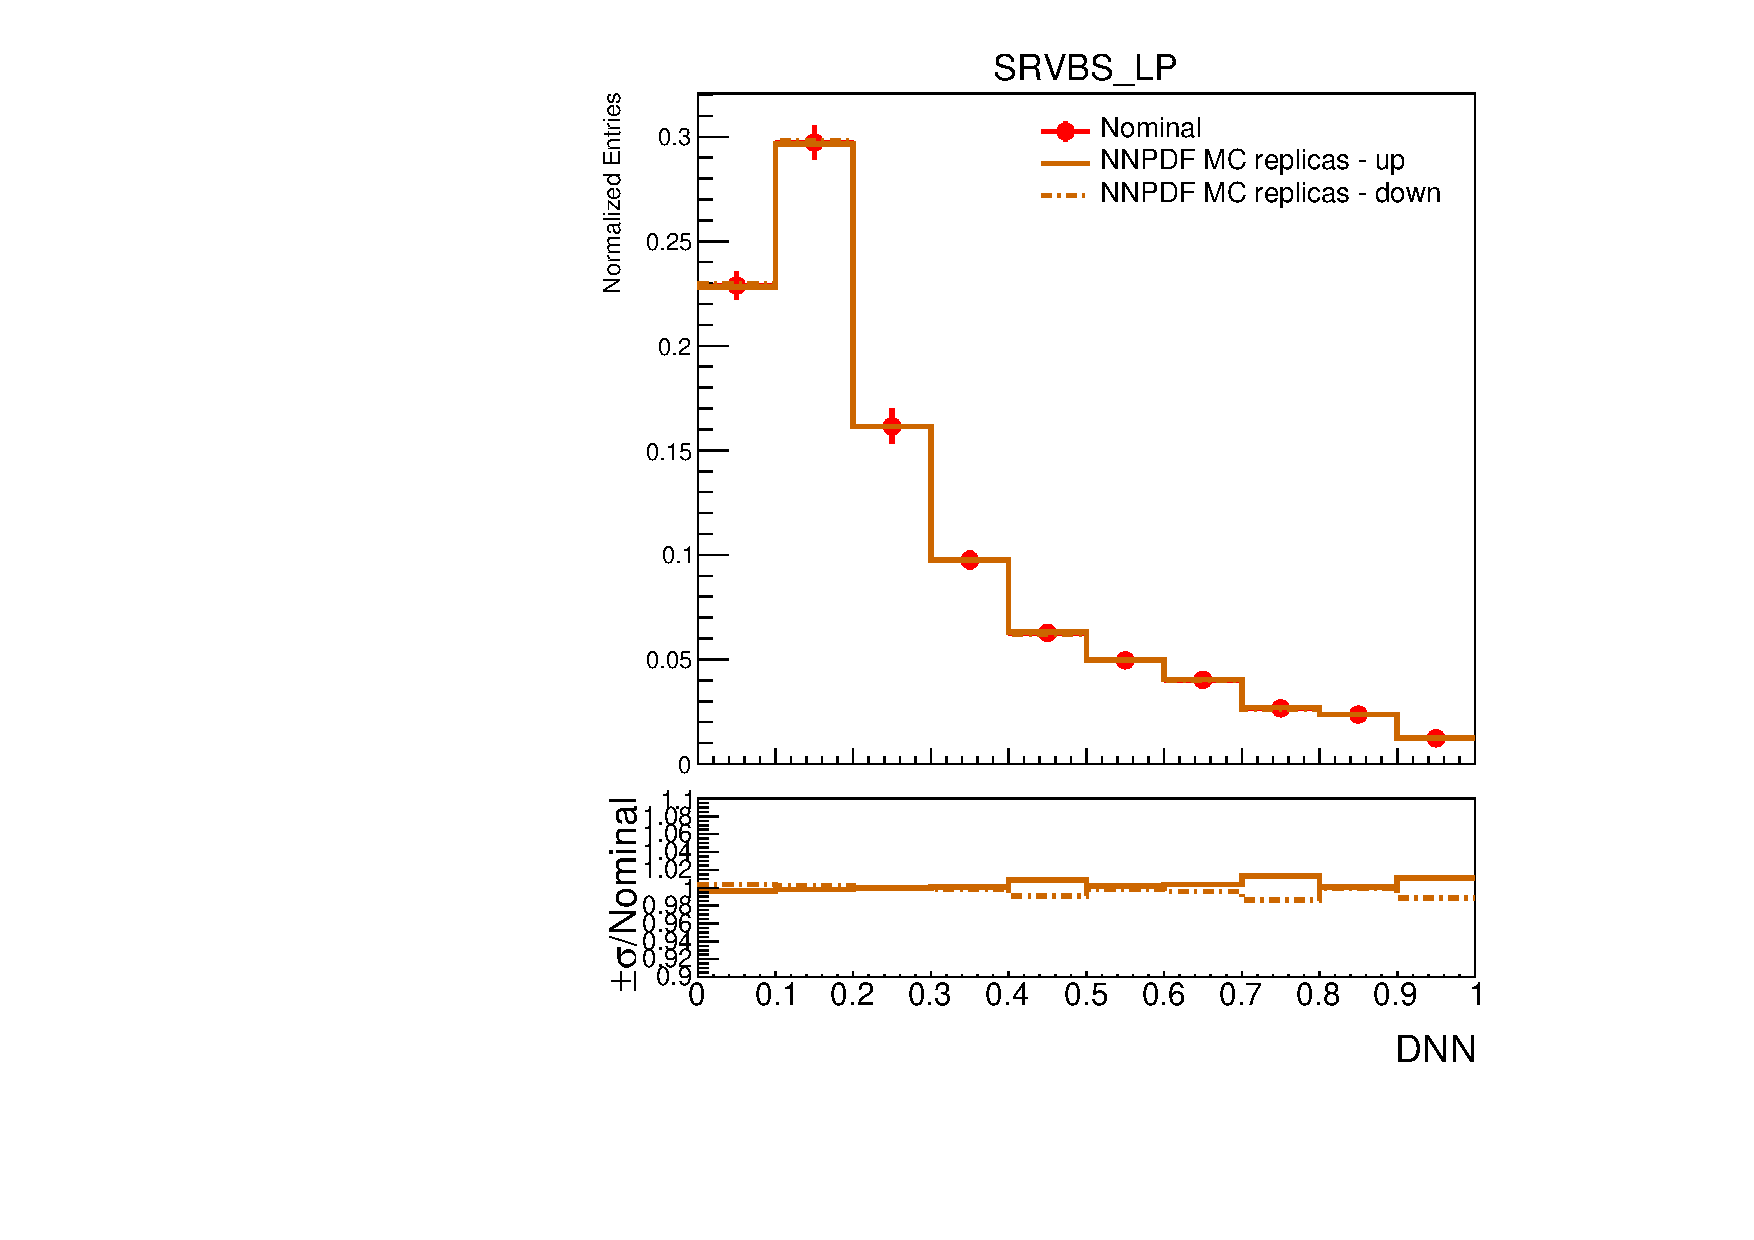
\includegraphics[width=\textwidth]{figures/1lep/PDFUnc/NNPDF/Z_0ptag1pfat0pjet_0ptv_SRVBS_LP_DNN_SysTheoryPDF_NNPDF_Z__1up_Norm.pdf}
        \caption{\Zjets, merged LP SR}
    \end{subfigure}
    \caption{PDF uncertainties using the NNPDF set in the 1-lepton channel. Histograms are normalized.}
    \label{fig:PDFUnc1Lep_bkg}
\end{figure}

\begin{figure}[ht]
    \centering
    \begin{subfigure}[b]{0.3\textwidth}
        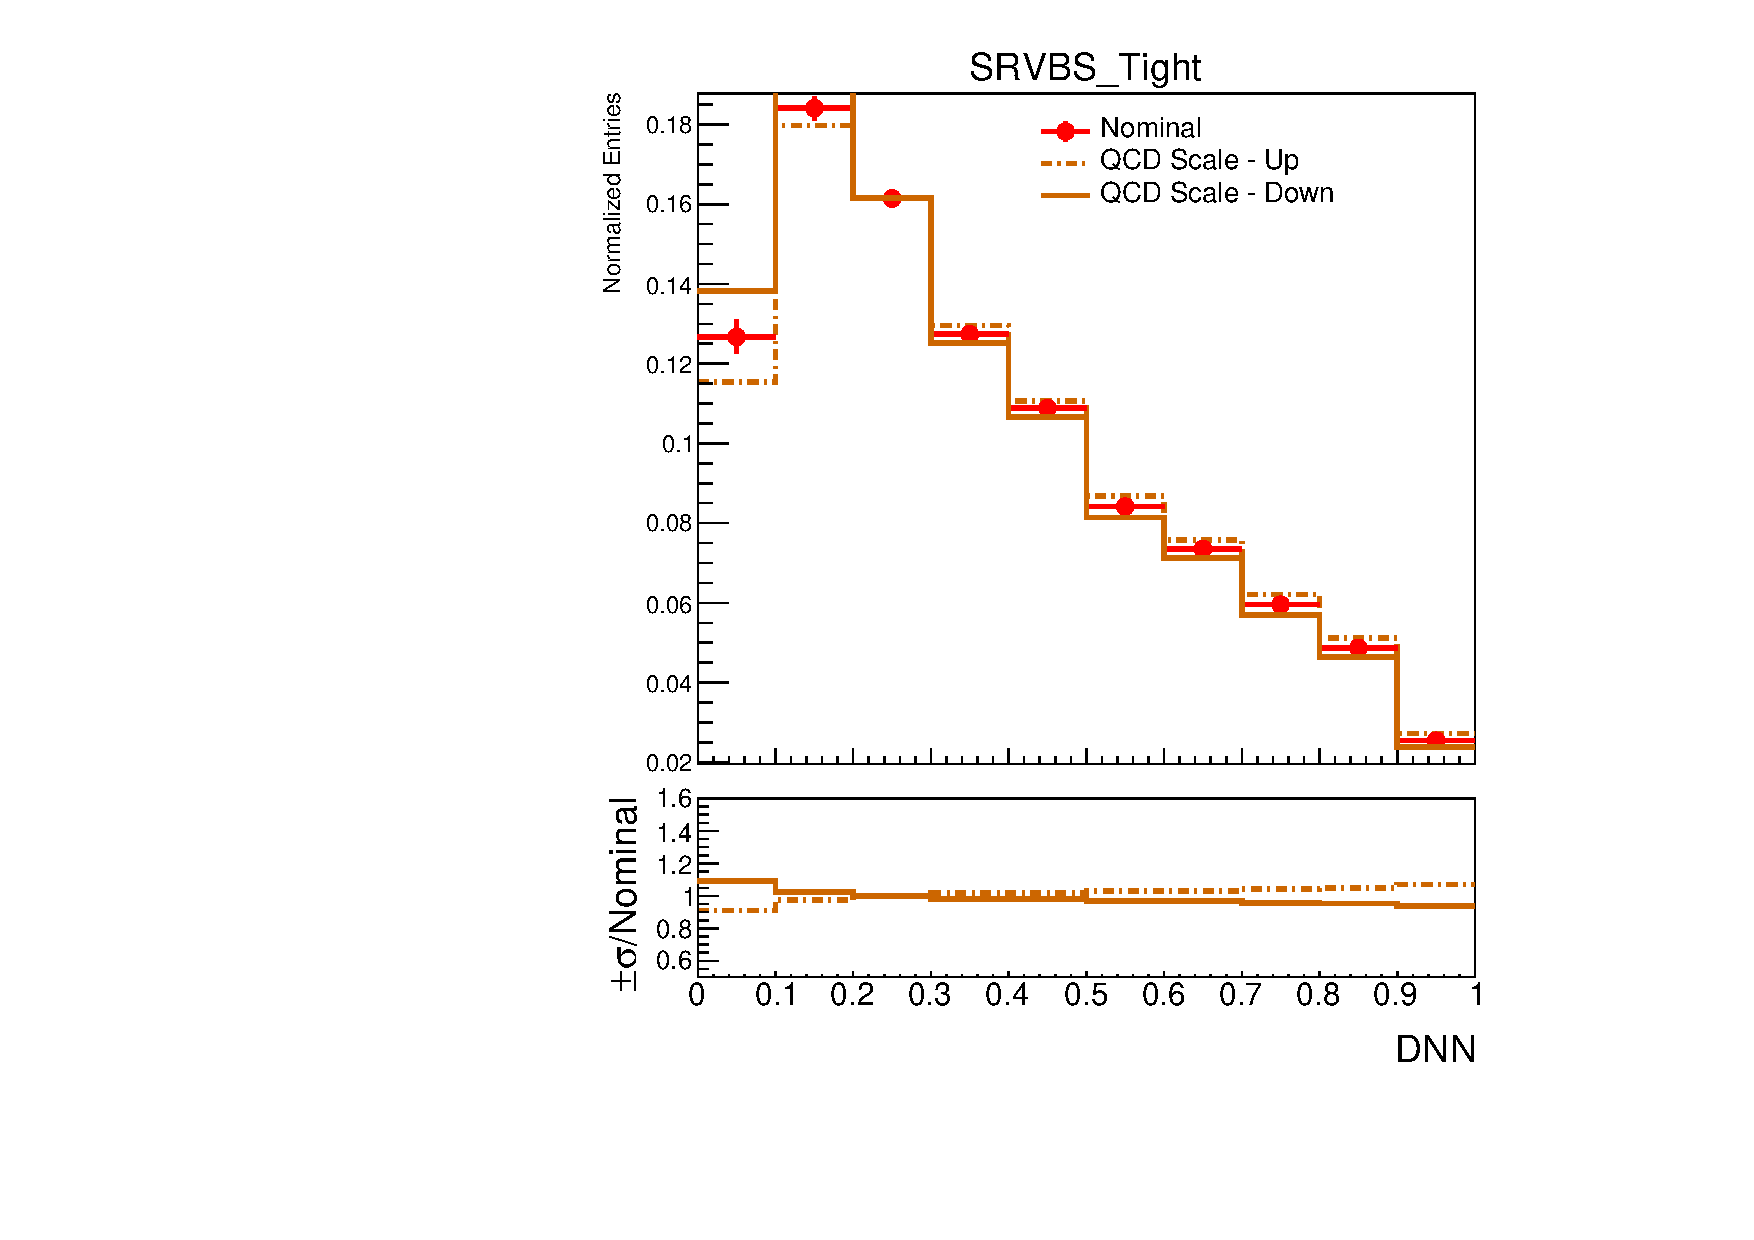
\includegraphics[width=\textwidth]{figures/1lep/PDFUnc/QCDScale/W_0ptag2pjet_0ptv_SRVBS_Tight_DNN_SysTheoryQCD_W__1up_Norm.pdf}
        \caption{\Wjets, resolved SR}
    \end{subfigure}
    \begin{subfigure}[b]{0.3\textwidth}
        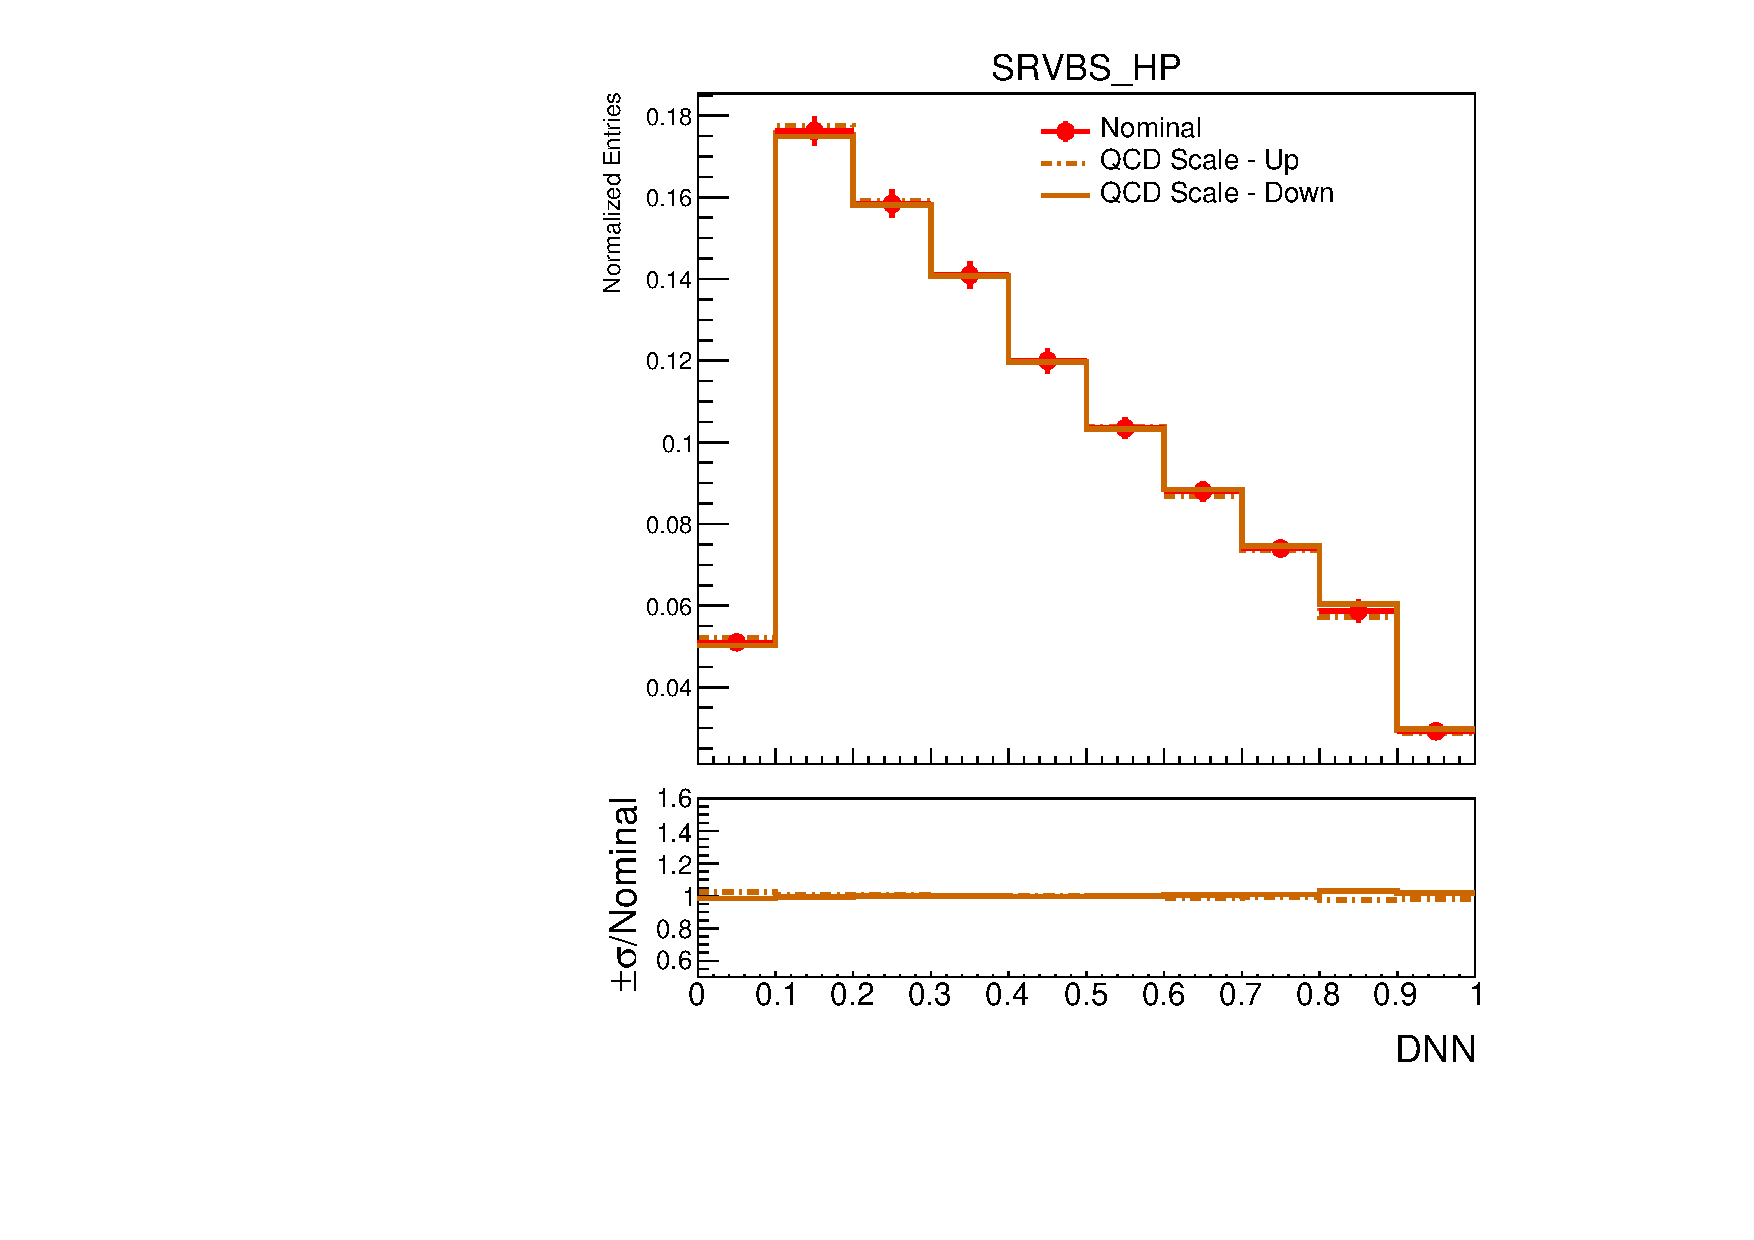
\includegraphics[width=\textwidth]{figures/1lep/PDFUnc/QCDScale/W_0ptag1pfat0pjet_0ptv_SRVBS_HP_DNN_SysTheoryQCD_W__1up_Norm.pdf}
        \caption{\Wjets, merged HP SR}
    \end{subfigure}
    \begin{subfigure}[b]{0.3\textwidth}
        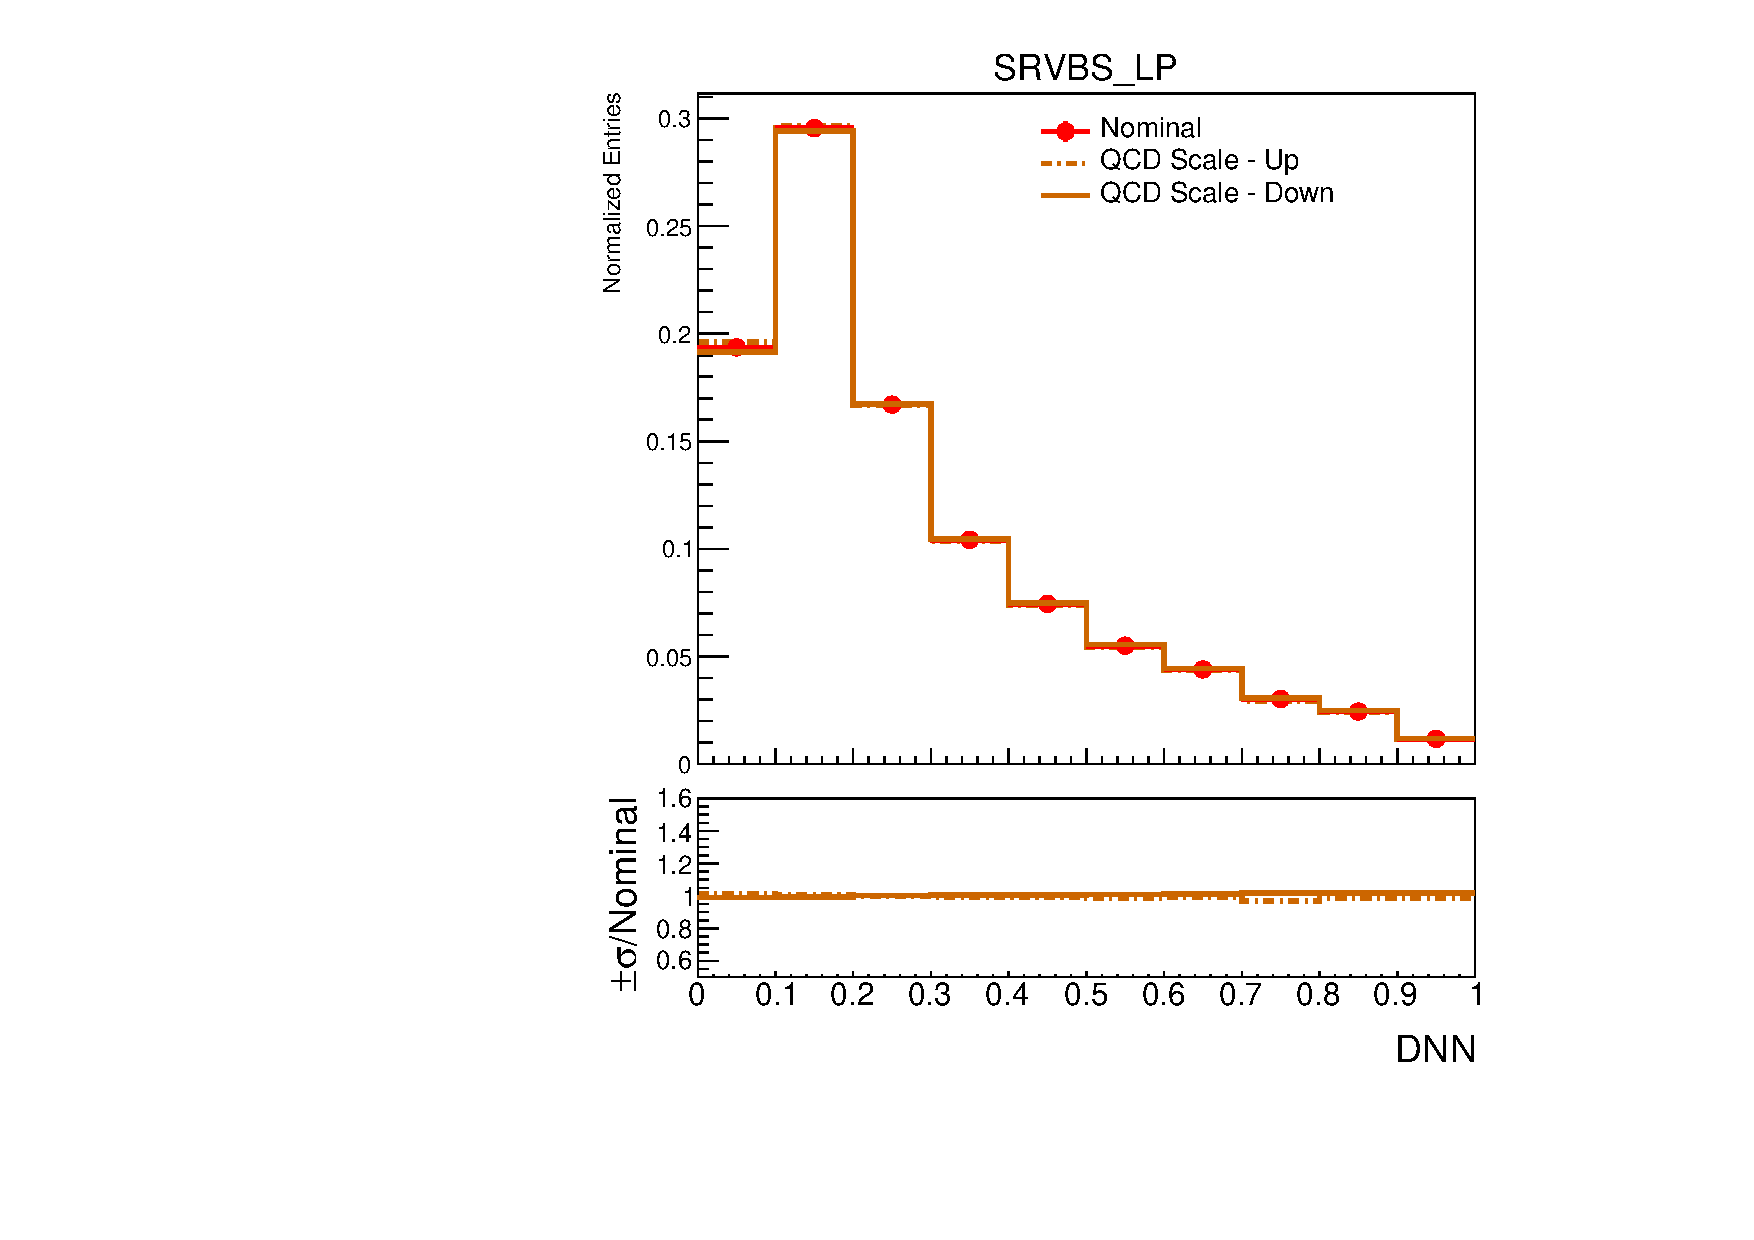
\includegraphics[width=\textwidth]{figures/1lep/PDFUnc/QCDScale/W_0ptag1pfat0pjet_0ptv_SRVBS_LP_DNN_SysTheoryQCD_W__1up_Norm.pdf}
        \caption{\Wjets, merged LP SR}
    \end{subfigure}
    \\
    \vspace{15mm}
    \begin{subfigure}[b]{0.3\textwidth}
        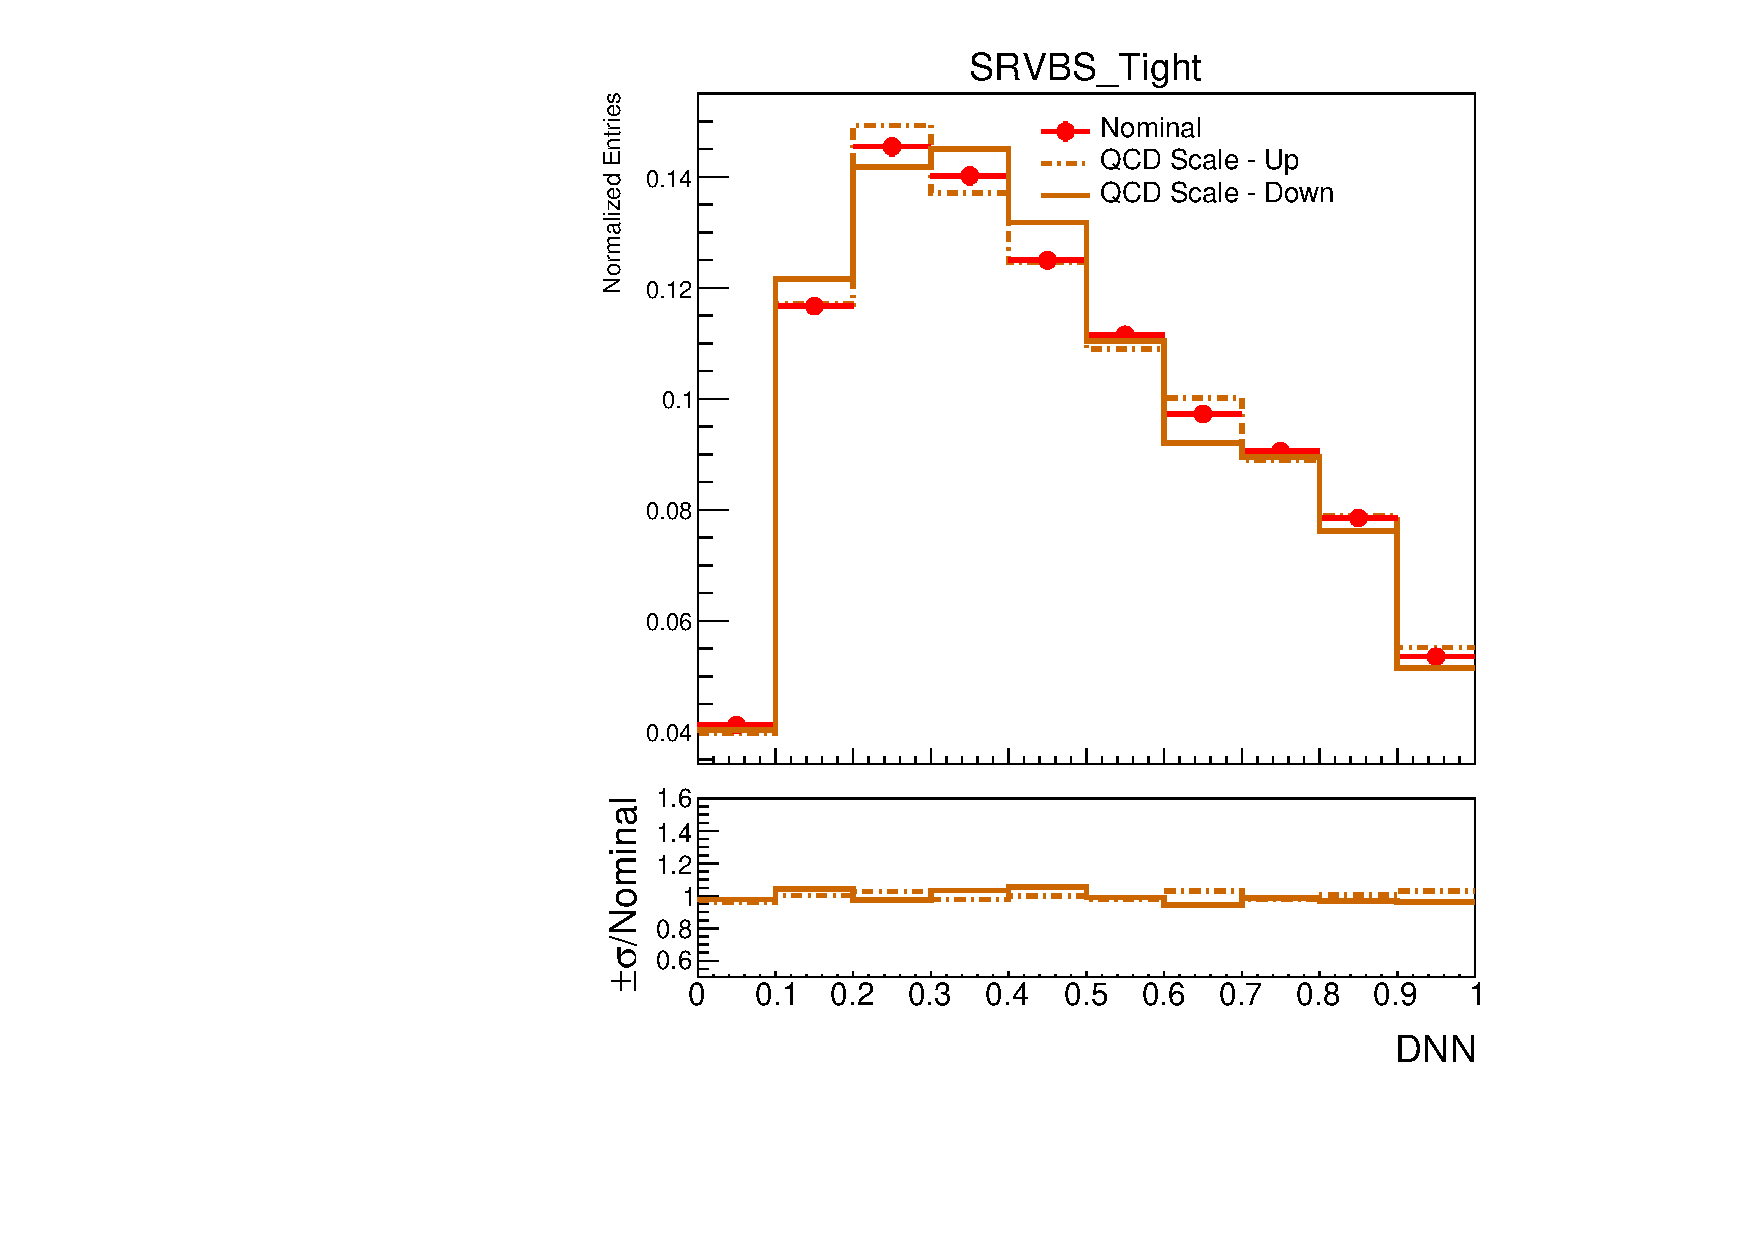
\includegraphics[width=\textwidth]{figures/1lep/PDFUnc/QCDScale/ttbar_0ptag2pjet_0ptv_SRVBS_Tight_DNN_SysTheoryQCD_ttbar__1up_Norm.pdf}
        \caption{\ttbar, resolved SR}
    \end{subfigure}
    \begin{subfigure}[b]{0.3\textwidth}
        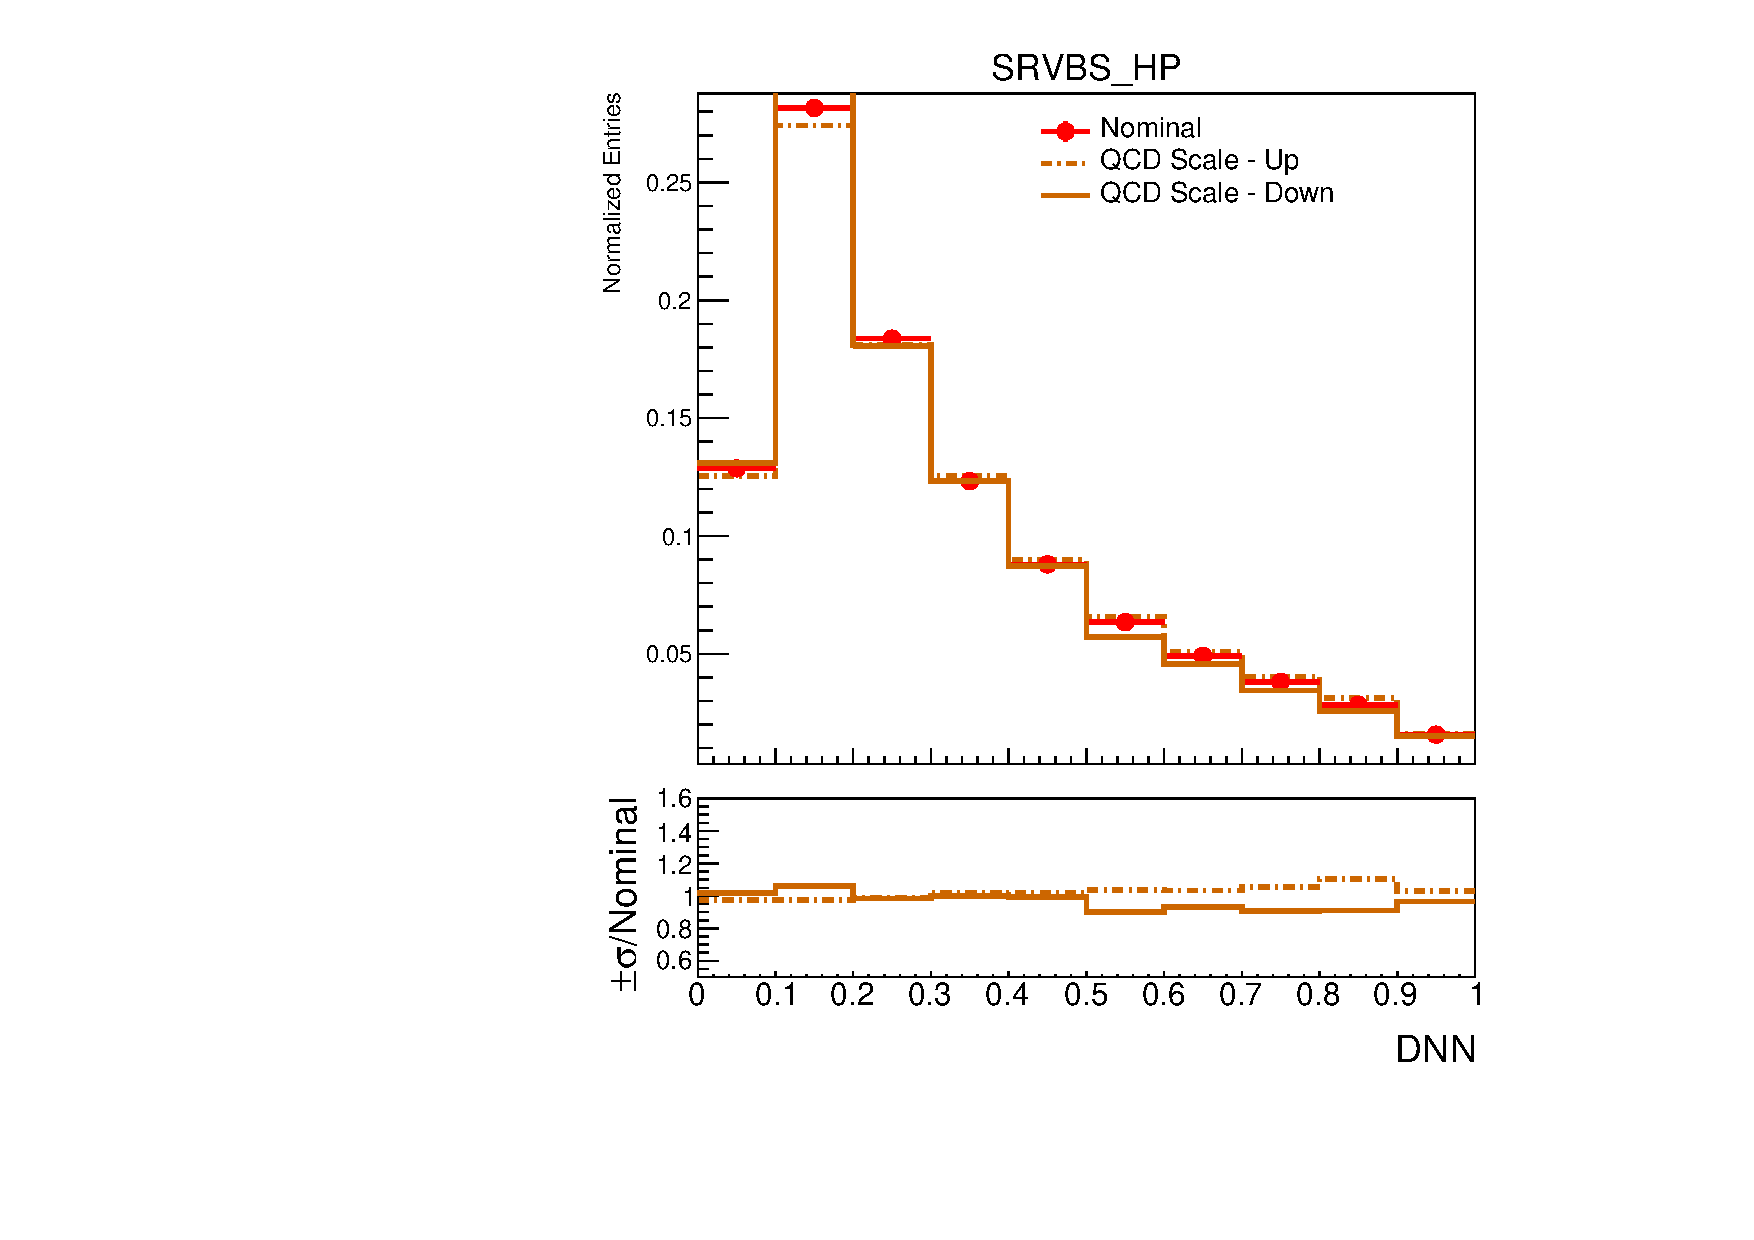
\includegraphics[width=\textwidth]{figures/1lep/PDFUnc/QCDScale/ttbar_0ptag1pfat0pjet_0ptv_SRVBS_HP_DNN_SysTheoryQCD_ttbar__1up_Norm.pdf}
        \caption{\ttbar, merged HP SR}
    \end{subfigure}
    \begin{subfigure}[b]{0.3\textwidth}
        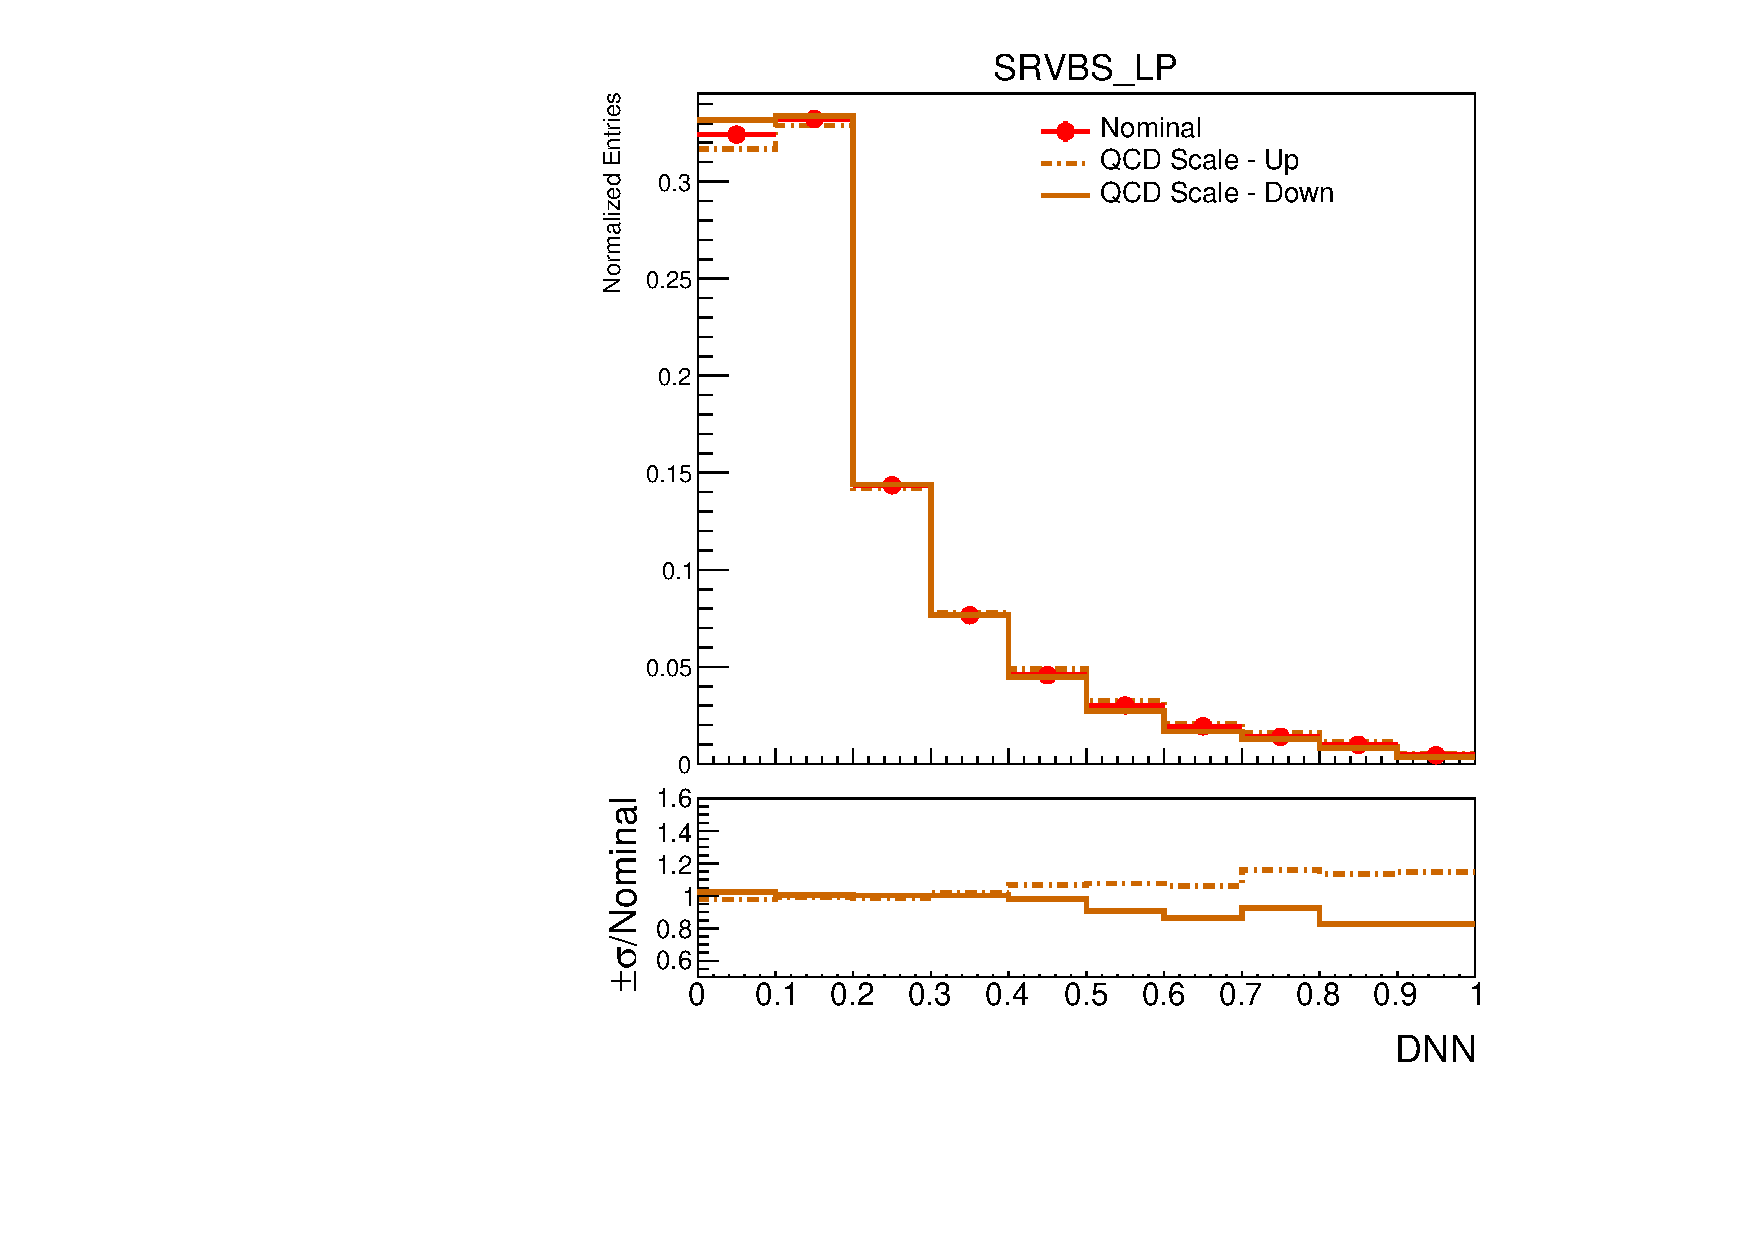
\includegraphics[width=\textwidth]{figures/1lep/PDFUnc/QCDScale/ttbar_0ptag1pfat0pjet_0ptv_SRVBS_LP_DNN_SysTheoryQCD_ttbar__1up_Norm.pdf}
        \caption{\ttbar, merged LP SR}
    \end{subfigure}
    \\
    \vspace{15mm}
    \begin{subfigure}[b]{0.3\textwidth}
        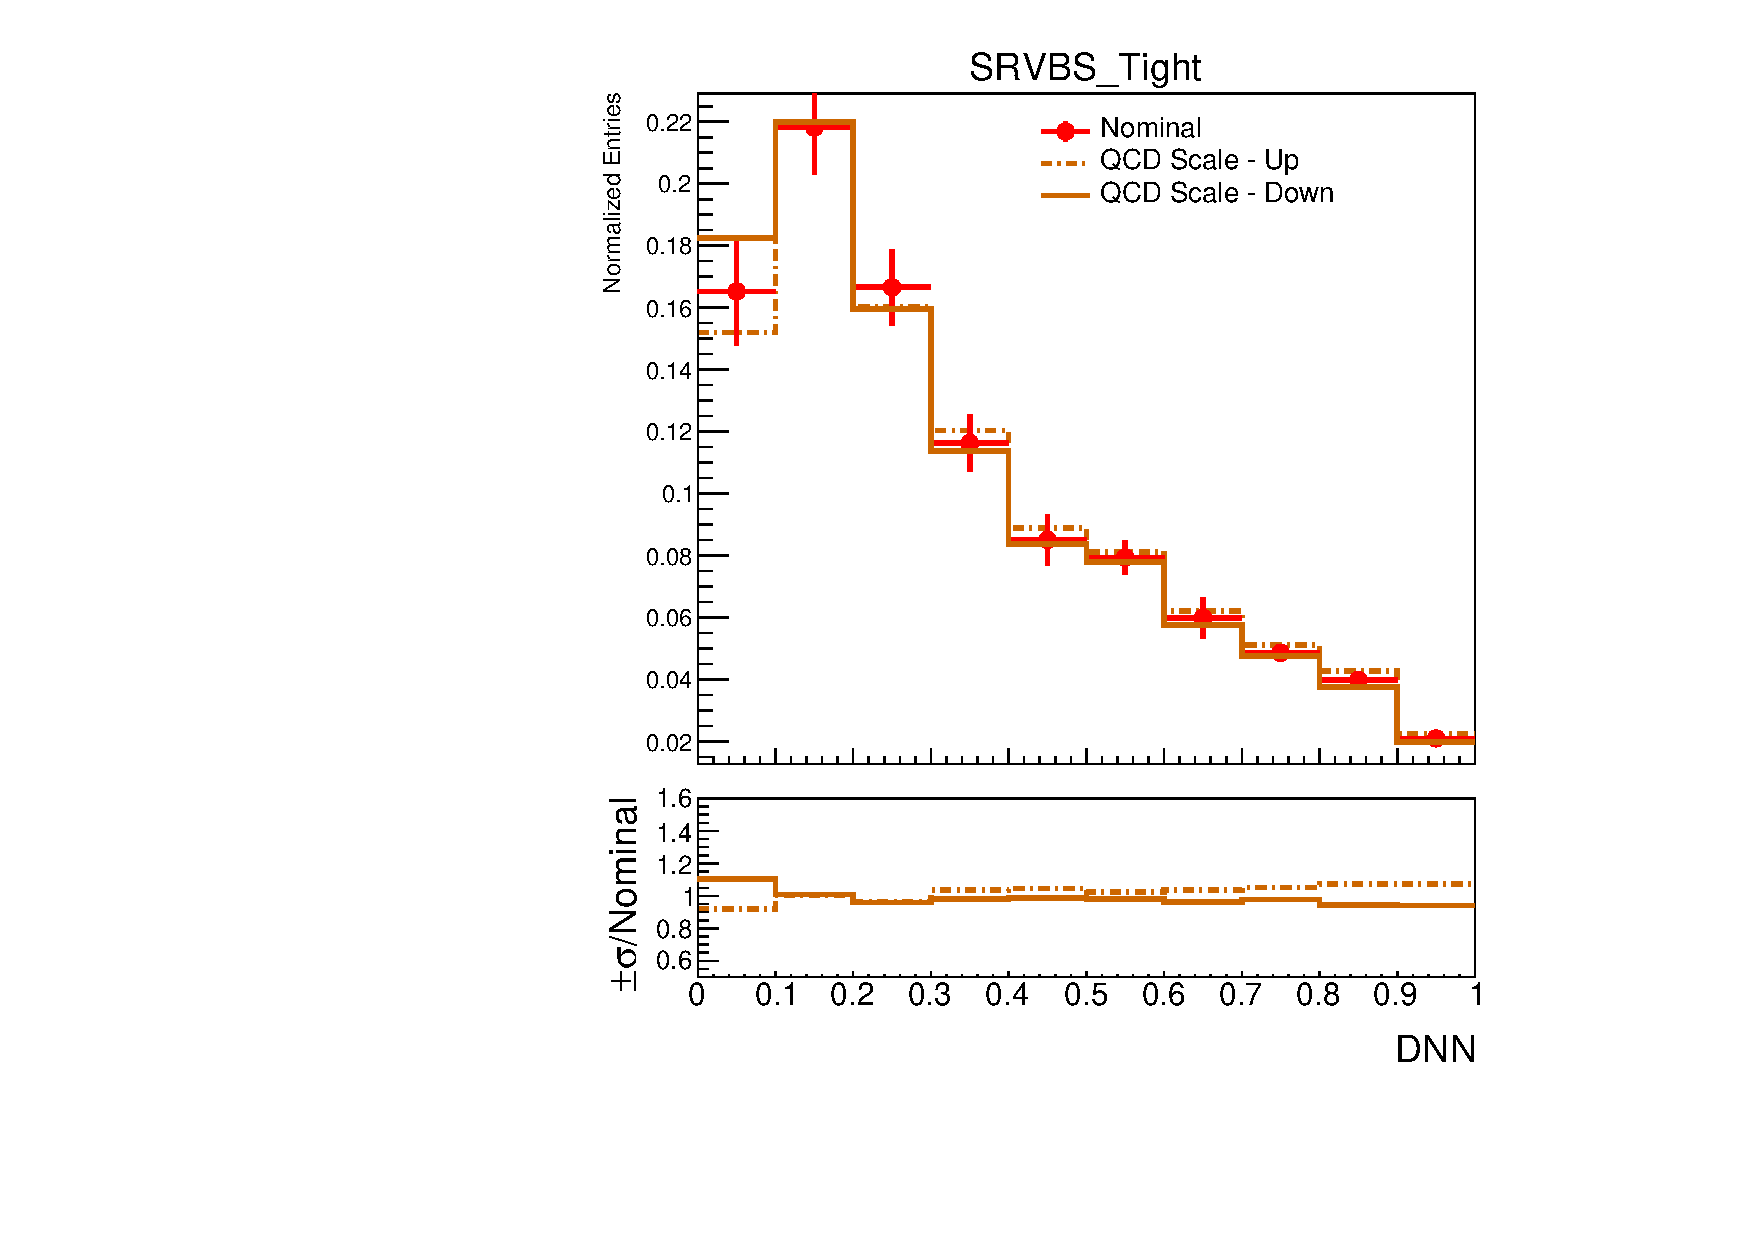
\includegraphics[width=\textwidth]{figures/1lep/PDFUnc/QCDScale/Z_0ptag2pjet_0ptv_SRVBS_Tight_DNN_SysTheoryQCD_Z__1up_Norm.pdf}
        \caption{\Zjets, resolved SR}
    \end{subfigure}
    \begin{subfigure}[b]{0.3\textwidth}
        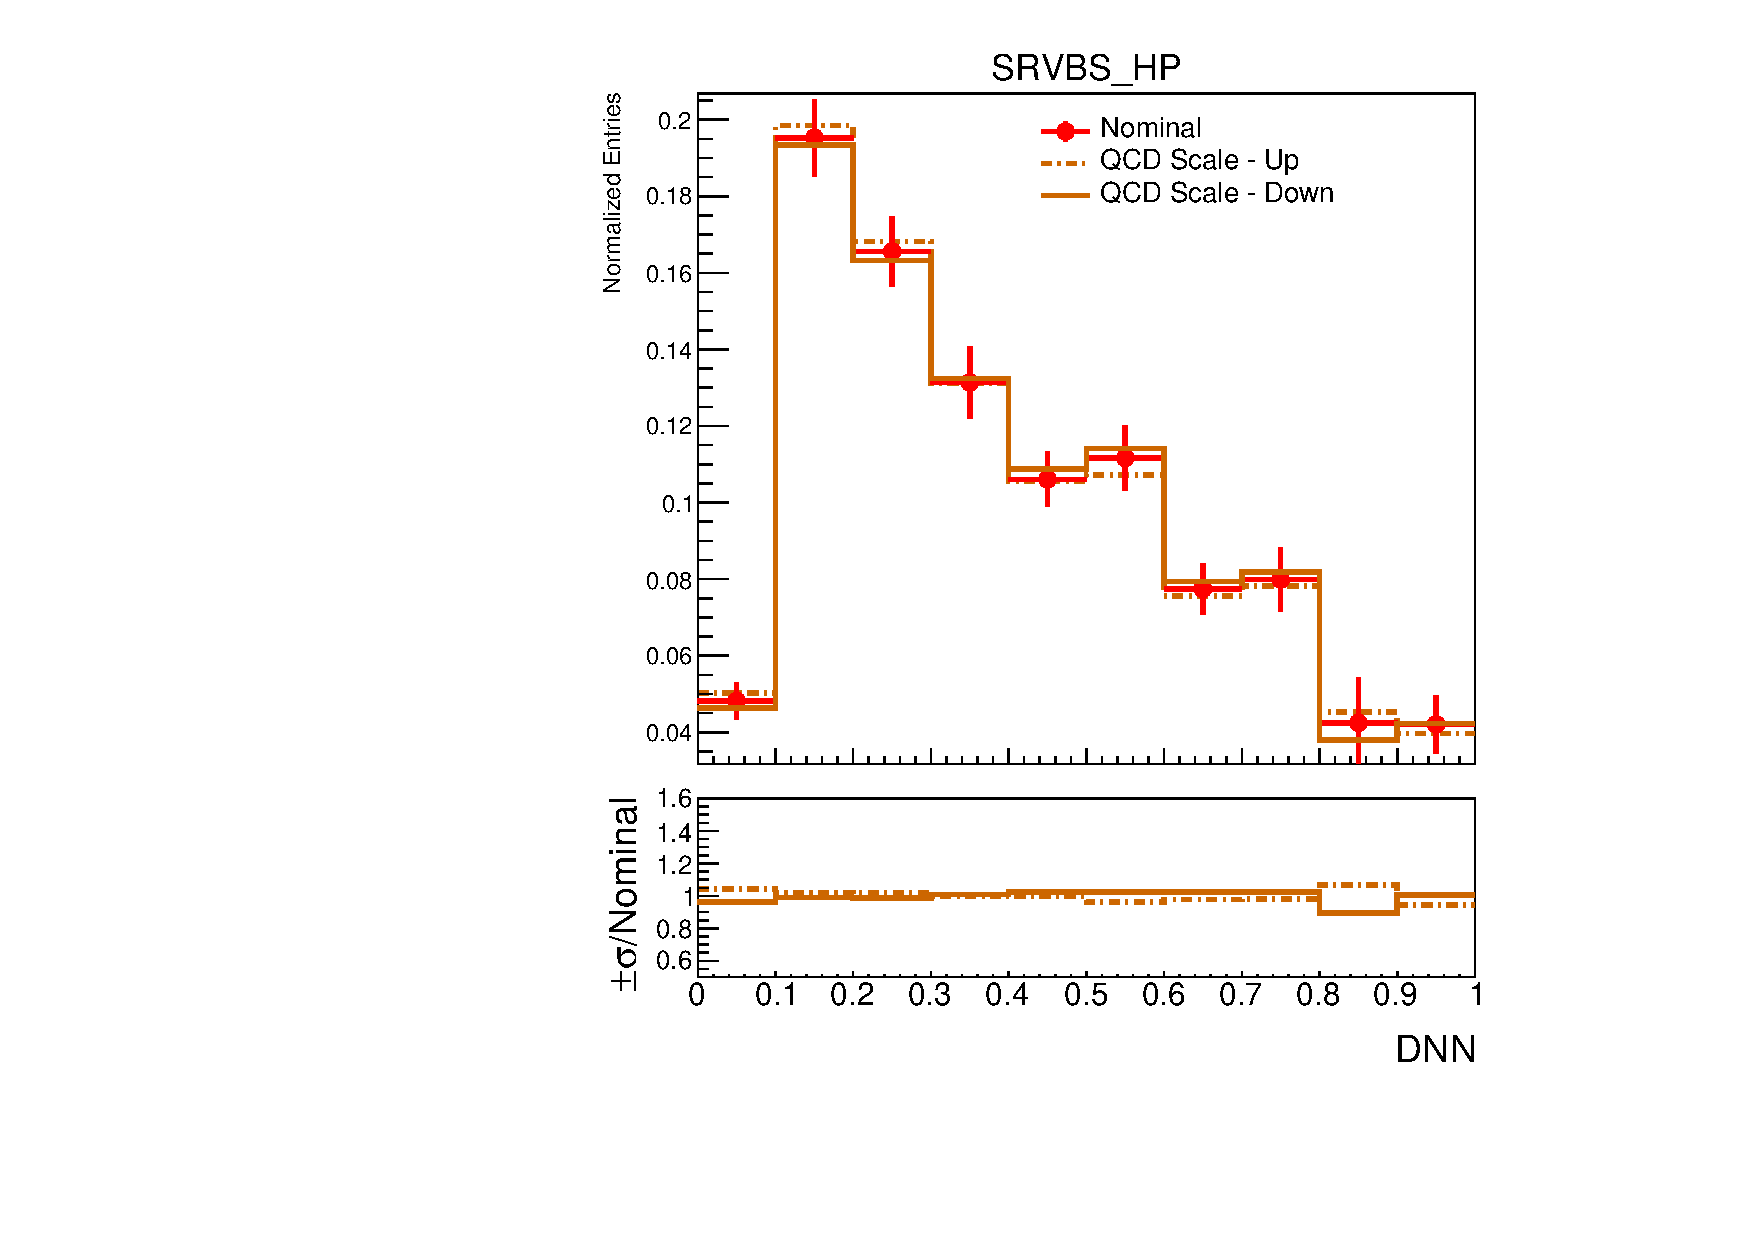
\includegraphics[width=\textwidth]{figures/1lep/PDFUnc/QCDScale/Z_0ptag1pfat0pjet_0ptv_SRVBS_HP_DNN_SysTheoryQCD_Z__1up_Norm.pdf}
        \caption{\Zjets, merged HP SR}
    \end{subfigure}
    \begin{subfigure}[b]{0.3\textwidth}
        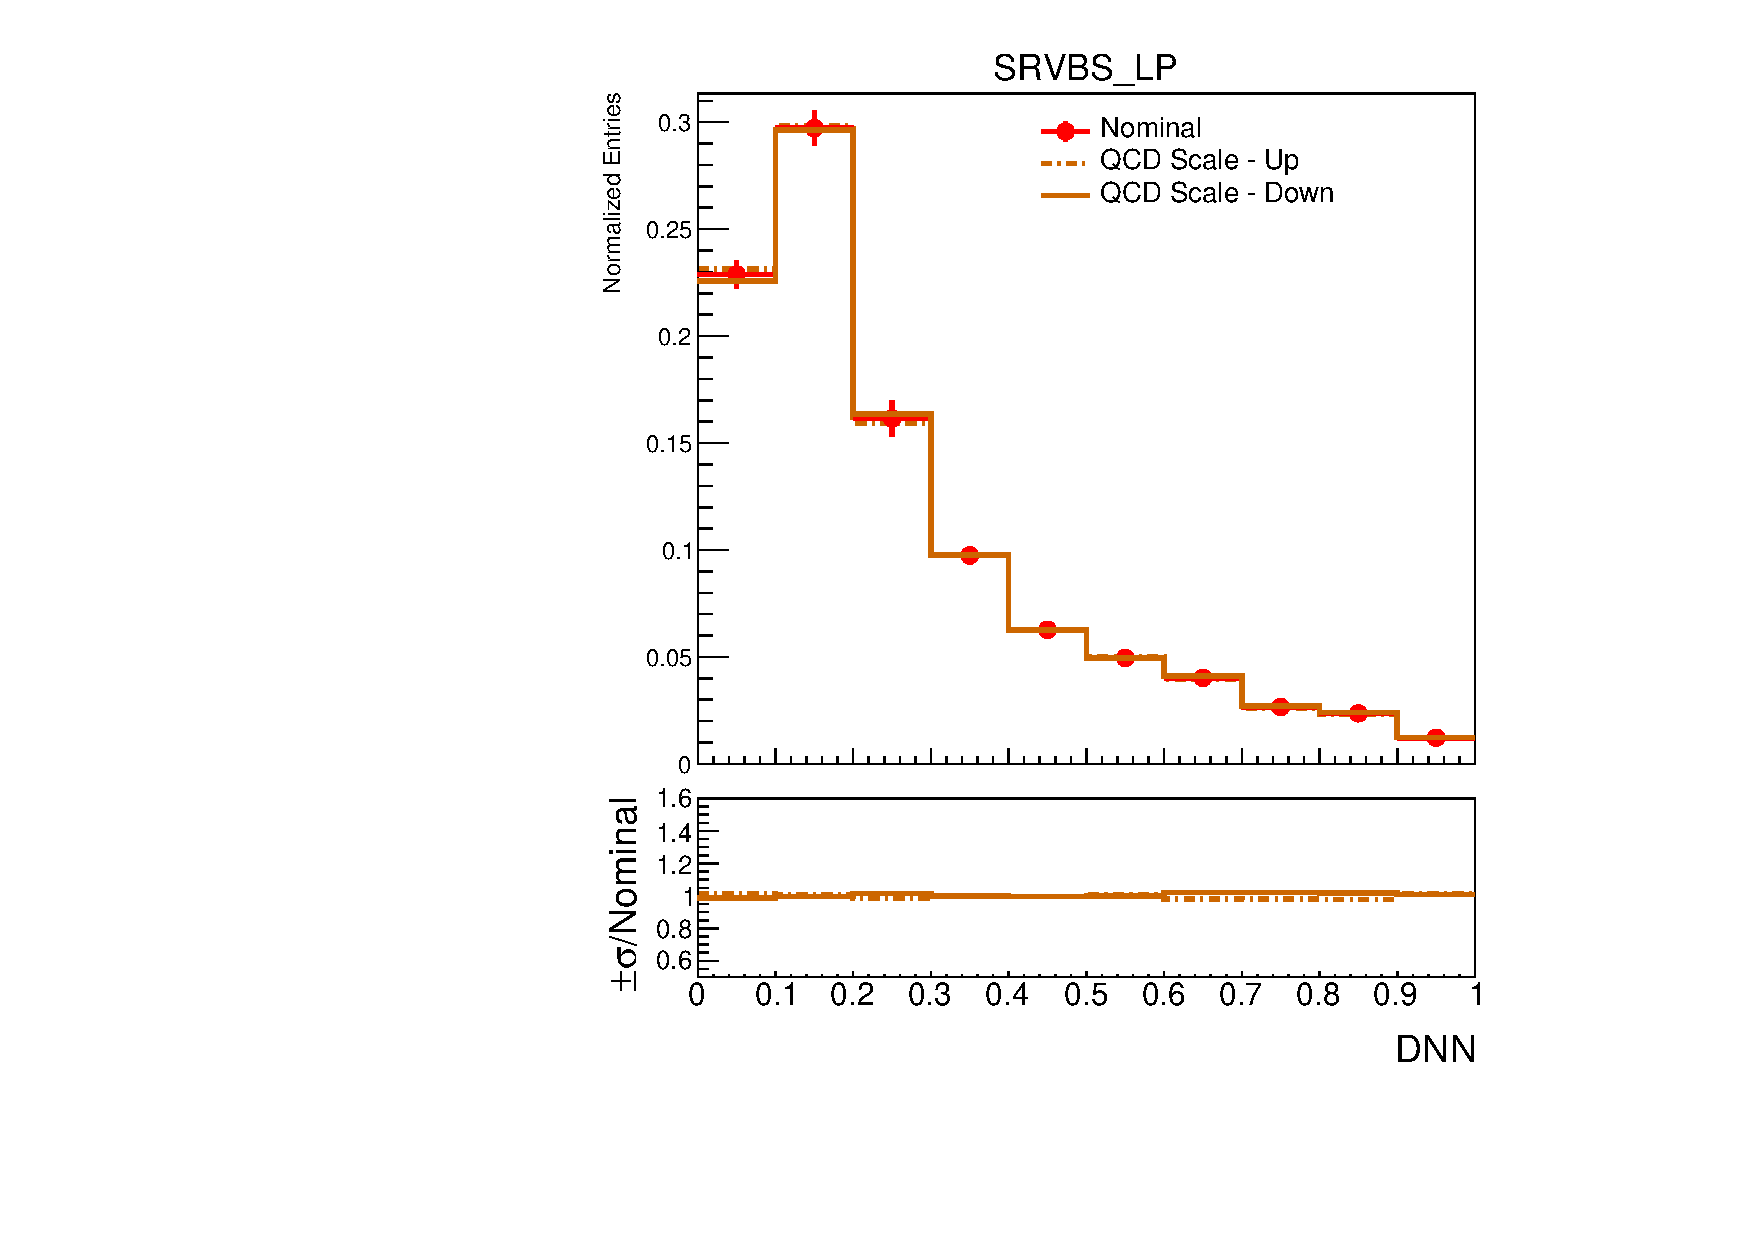
\includegraphics[width=\textwidth]{figures/1lep/PDFUnc/QCDScale/Z_0ptag1pfat0pjet_0ptv_SRVBS_LP_DNN_SysTheoryQCD_Z__1up_Norm.pdf}
        \caption{\Zjets, merged LP SR}
    \end{subfigure}
    \caption{QCD scale uncertainties in the 1-lepton channel. Histograms are normalized.}
    \label{fig:PDFUnc1Lep_QCD}
\end{figure}

\clearpage
\subsection{ISR/FSR uncertainties}
\label{subsec:isr_fsr_unc}

The impact of initial and final state radiation (ISR/FSR) on top quark backgrounds is investigated using dedicated samples that vary the amount of additional radiation.
Figures \ref{fig:isrUnc1Lep} and \ref{fig:fsrUnc1Lep} illustrate the effects of ISR and FSR uncertainties in the 1-lepton channel.

%%%\begin{figure}[ht]
%%%    \centering
%%%    \begin{subfigure}[b]{0.3\textwidth}
%%%        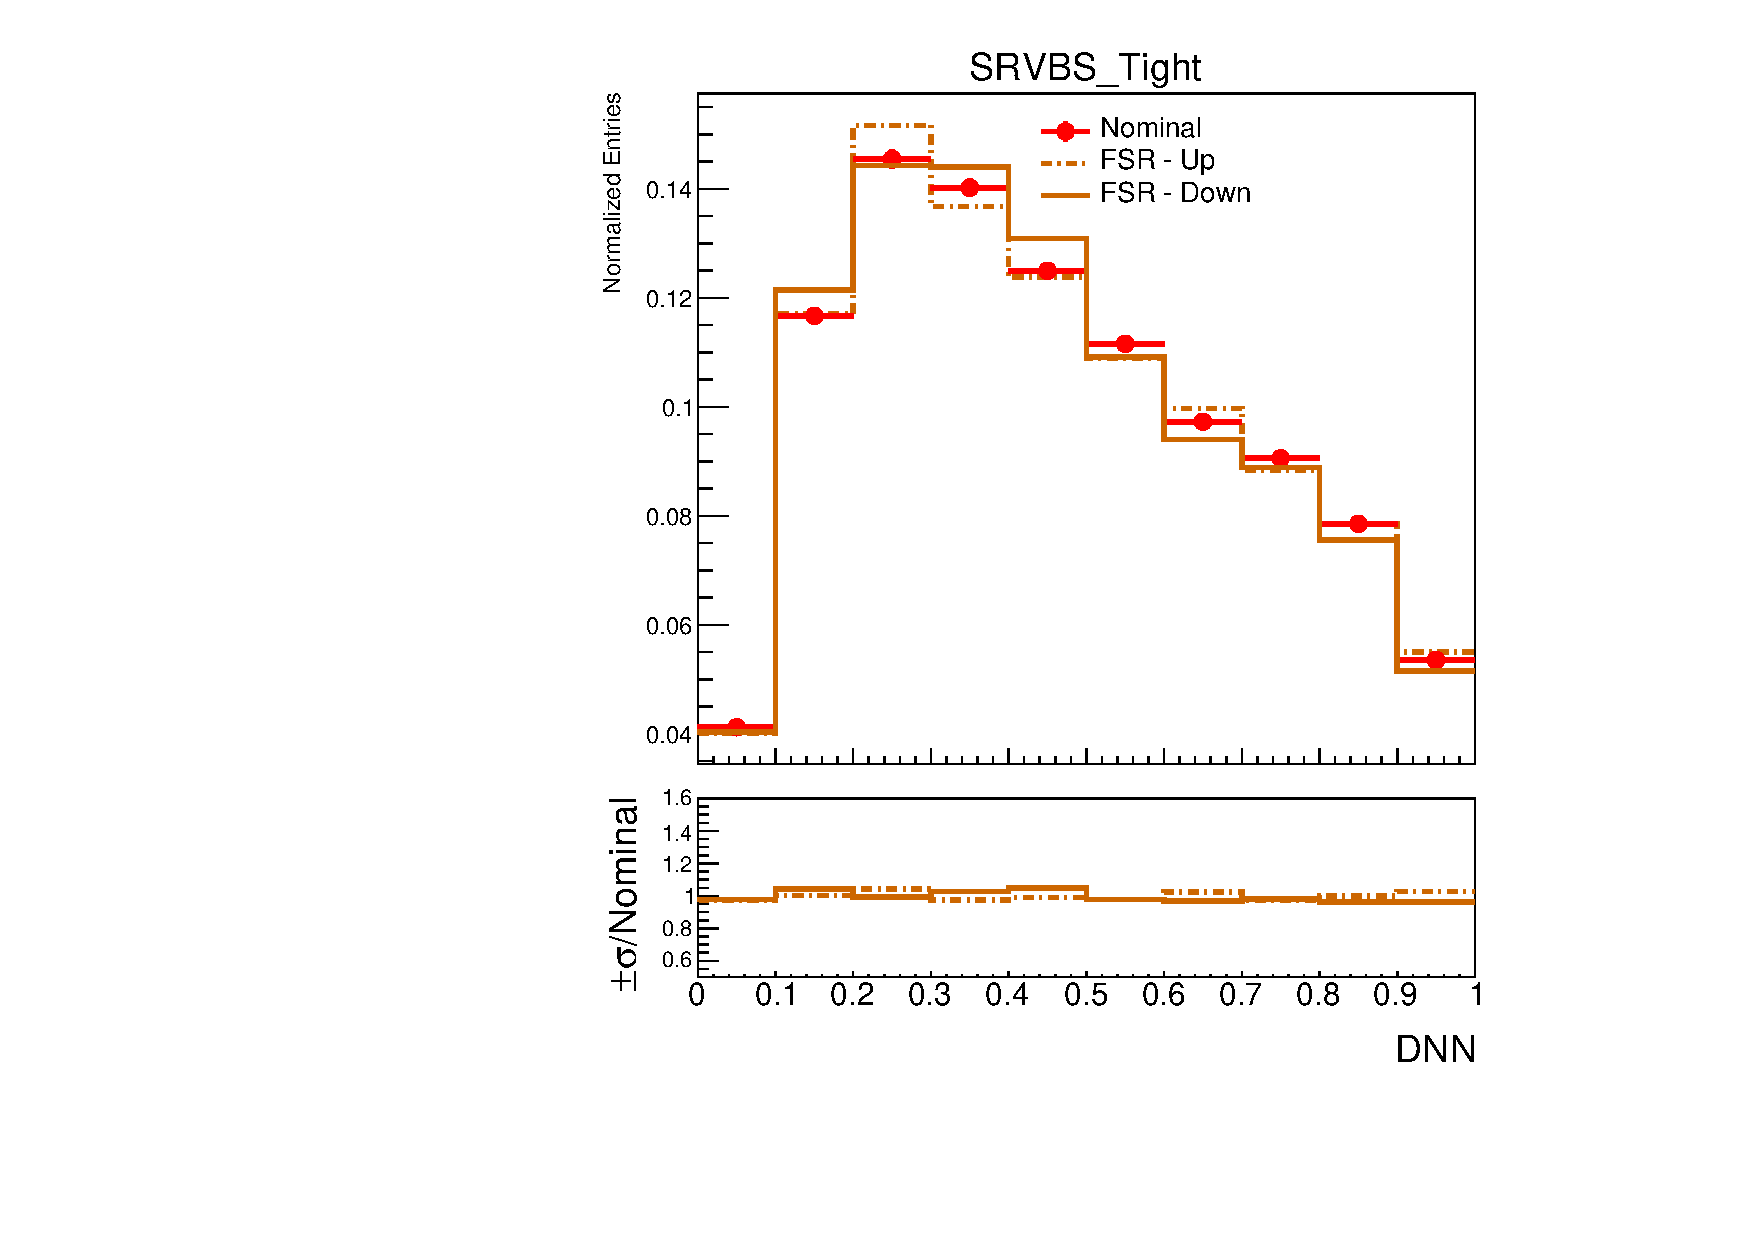
\includegraphics[width=\textwidth]{figures/1lep/PDFUnc/FSR/ttbar_0ptag2pjet_0ptv_SRVBS_Tight_DNN_SysTheoryFSR_Top__1up_Norm.pdf}
%%%        \caption{\ttbar, resolved SR}
%%%    \end{subfigure}
%%%    \begin{subfigure}[b]{0.3\textwidth}
%%%        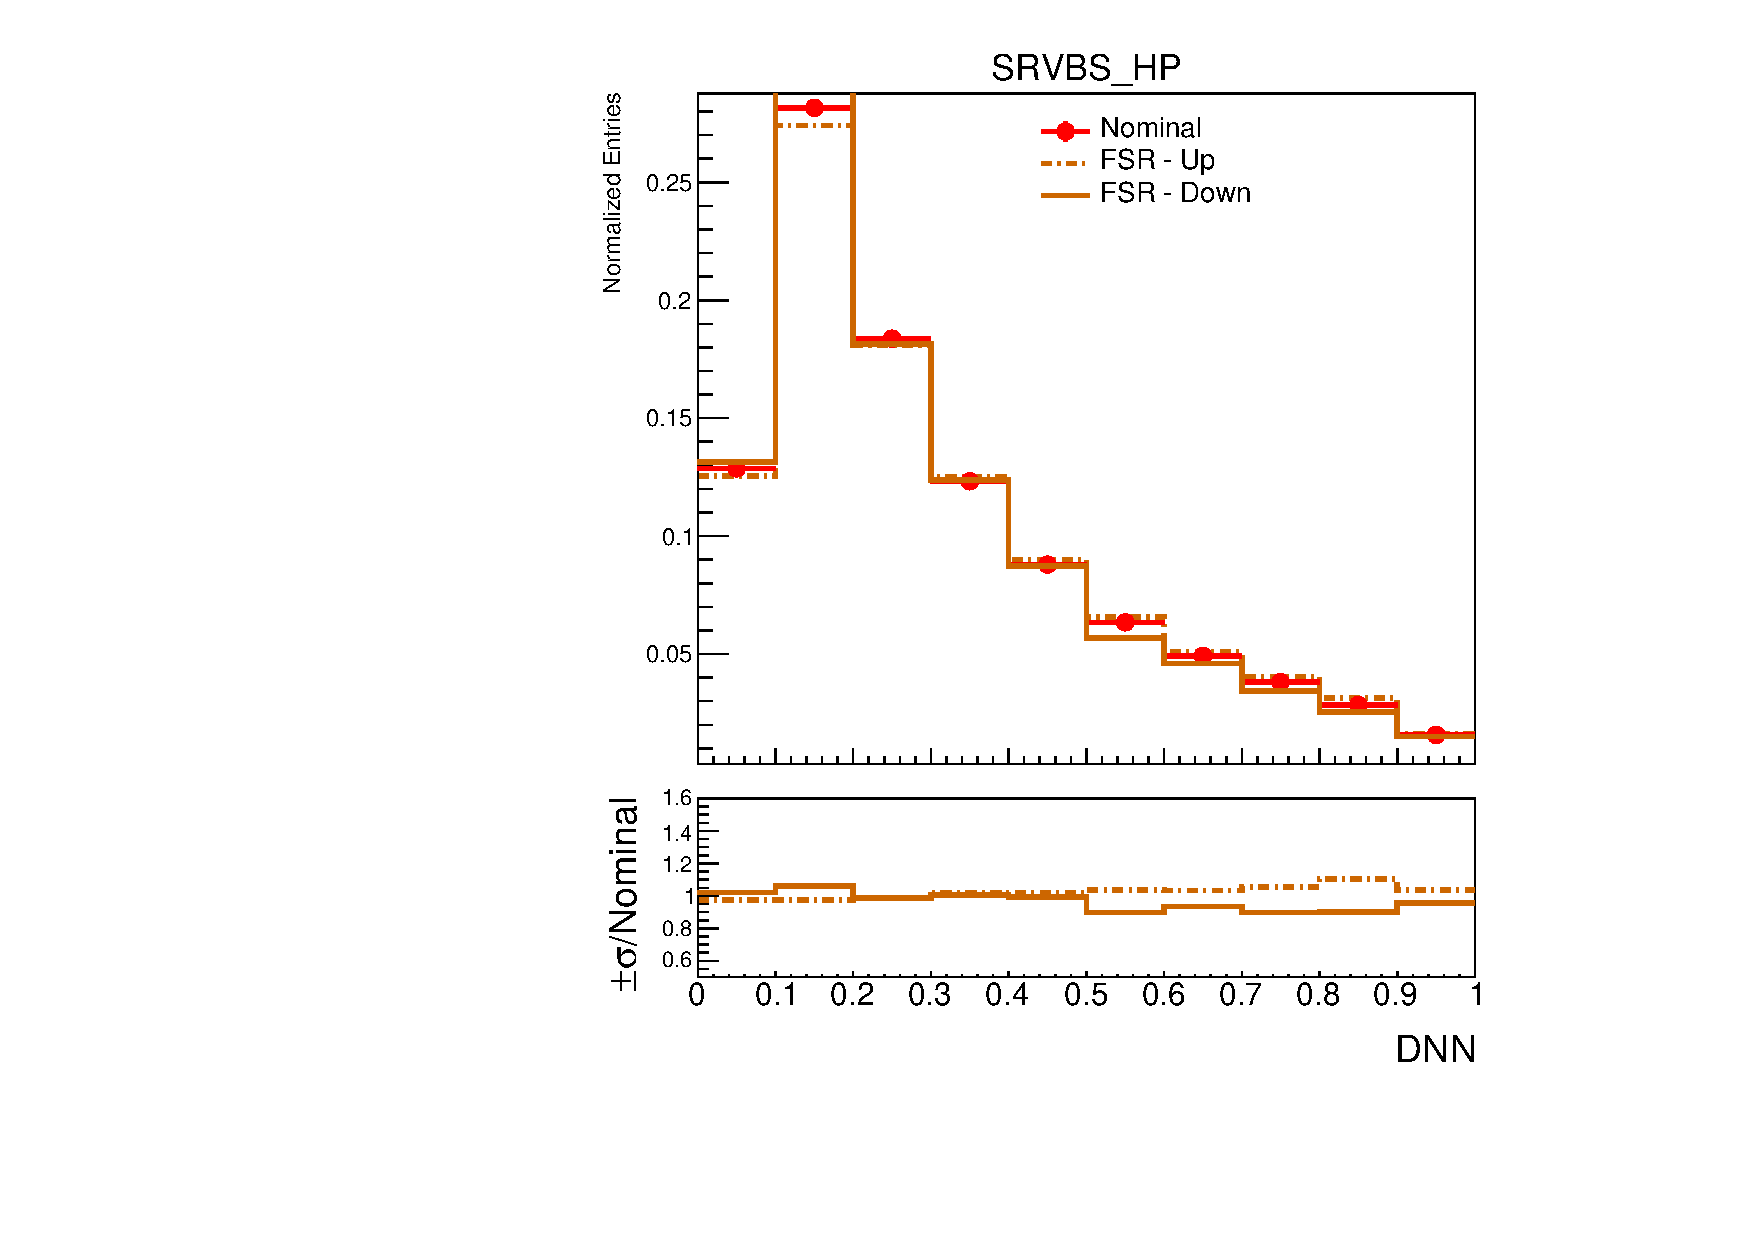
\includegraphics[width=\textwidth]{figures/1lep/PDFUnc/FSR/ttbar_0ptag1pfat0pjet_0ptv_SRVBS_HP_DNN_SysTheoryFSR_Top__1up_Norm.pdf}
%%%        \caption{\ttbar, merged HP SR}
%%%    \end{subfigure}
%%%    \begin{subfigure}[b]{0.3\textwidth}
%%%        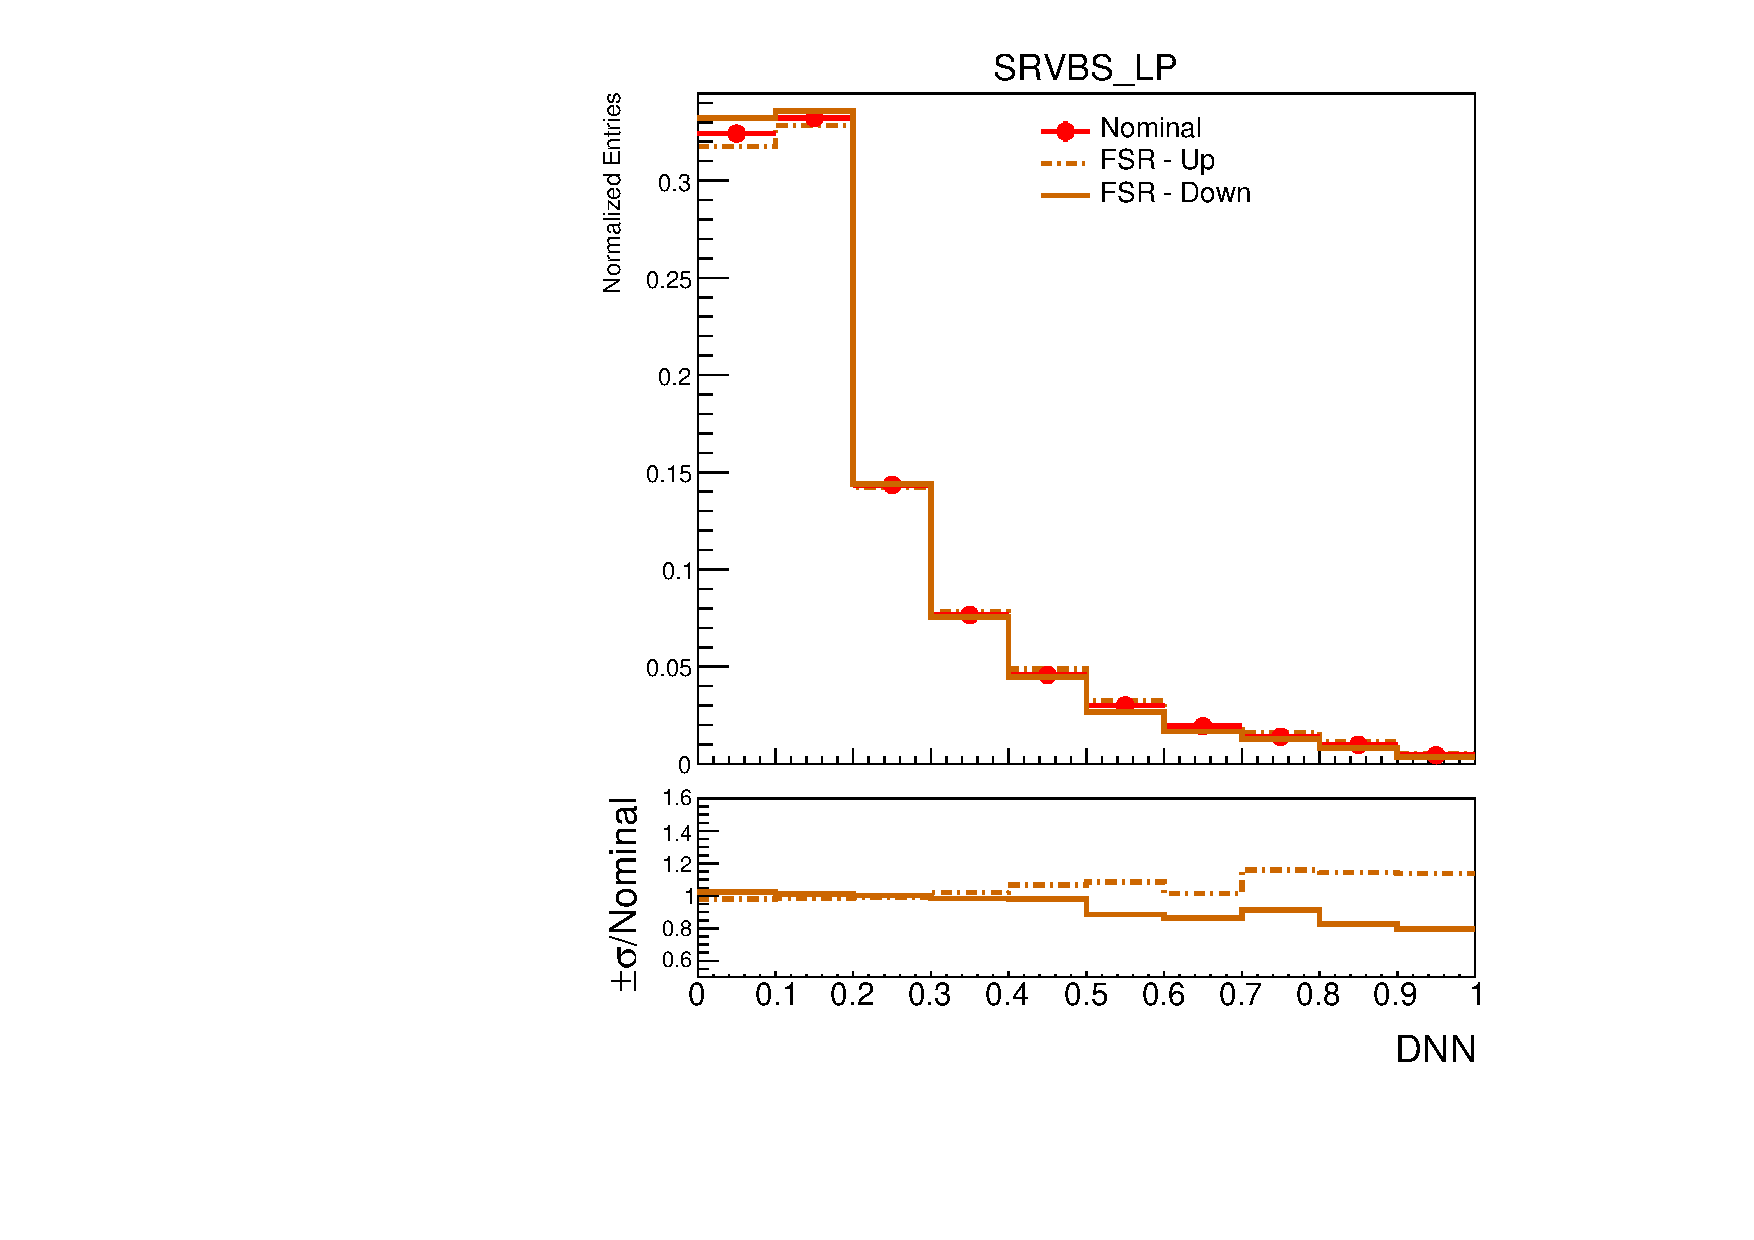
\includegraphics[width=\textwidth]{figures/1lep/PDFUnc/FSR/ttbar_0ptag1pfat0pjet_0ptv_SRVBS_LP_DNN_SysTheoryFSR_Top__1up_Norm.pdf}
%%%        \caption{\ttbar, merged LP SR}
%%%    \end{subfigure}
%%%    \label{fig:fsrUnc1Lep}
%%%\end{figure}


\begin{figure}[p]
    \centering
    \begin{subfigure}[b]{0.3\textwidth}
        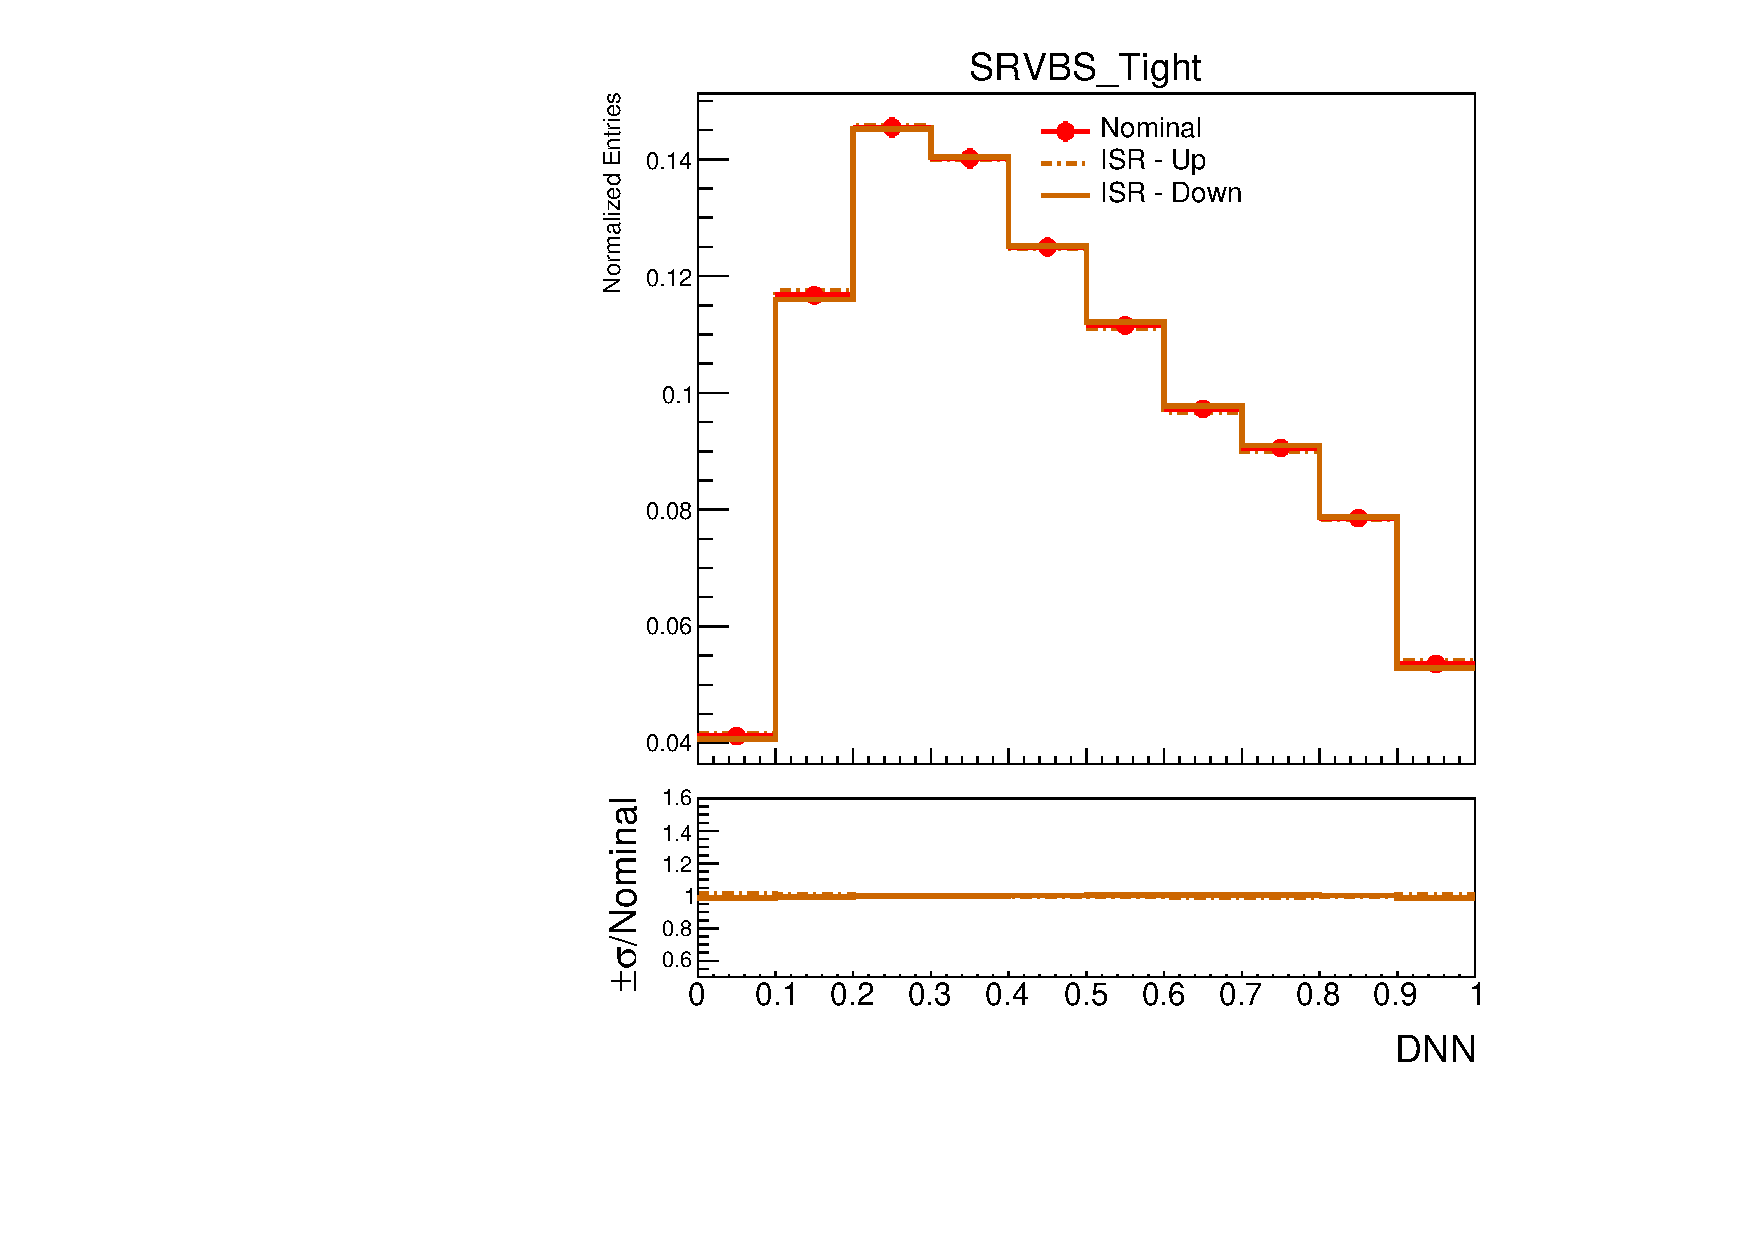
\includegraphics[width=\textwidth]{figures/1lep/PDFUnc/ISR/ttbar_0ptag2pjet_0ptv_SRVBS_Tight_DNN_SysTheoryISR_ttbar__1up_Norm.pdf}
        \caption{\ttbar, resolved SR}
    \end{subfigure}
    \begin{subfigure}[b]{0.3\textwidth}
        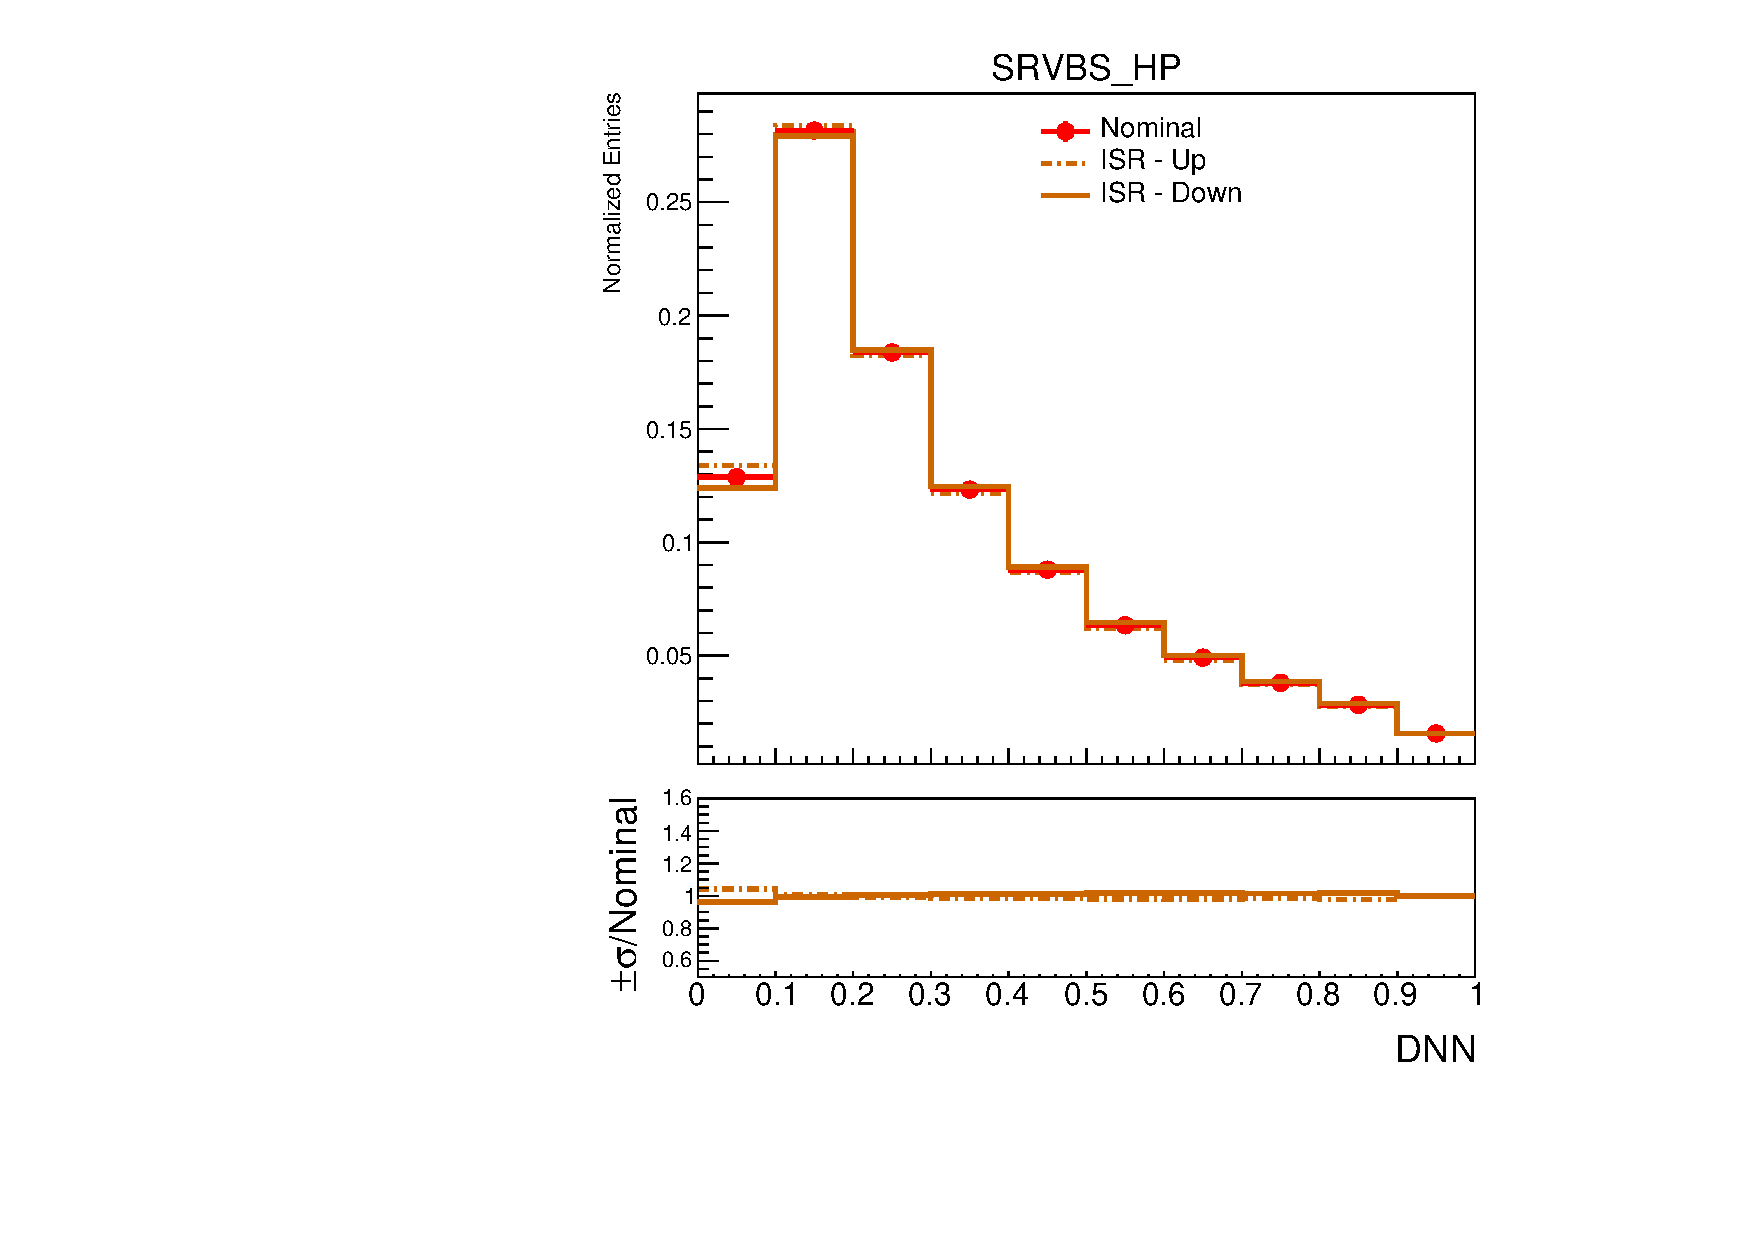
\includegraphics[width=\textwidth]{figures/1lep/PDFUnc/ISR/ttbar_0ptag1pfat0pjet_0ptv_SRVBS_HP_DNN_SysTheoryISR_ttbar__1up_Norm.pdf}
        \caption{\ttbar, merged HP SR}
    \end{subfigure}
    \begin{subfigure}[b]{0.3\textwidth}
        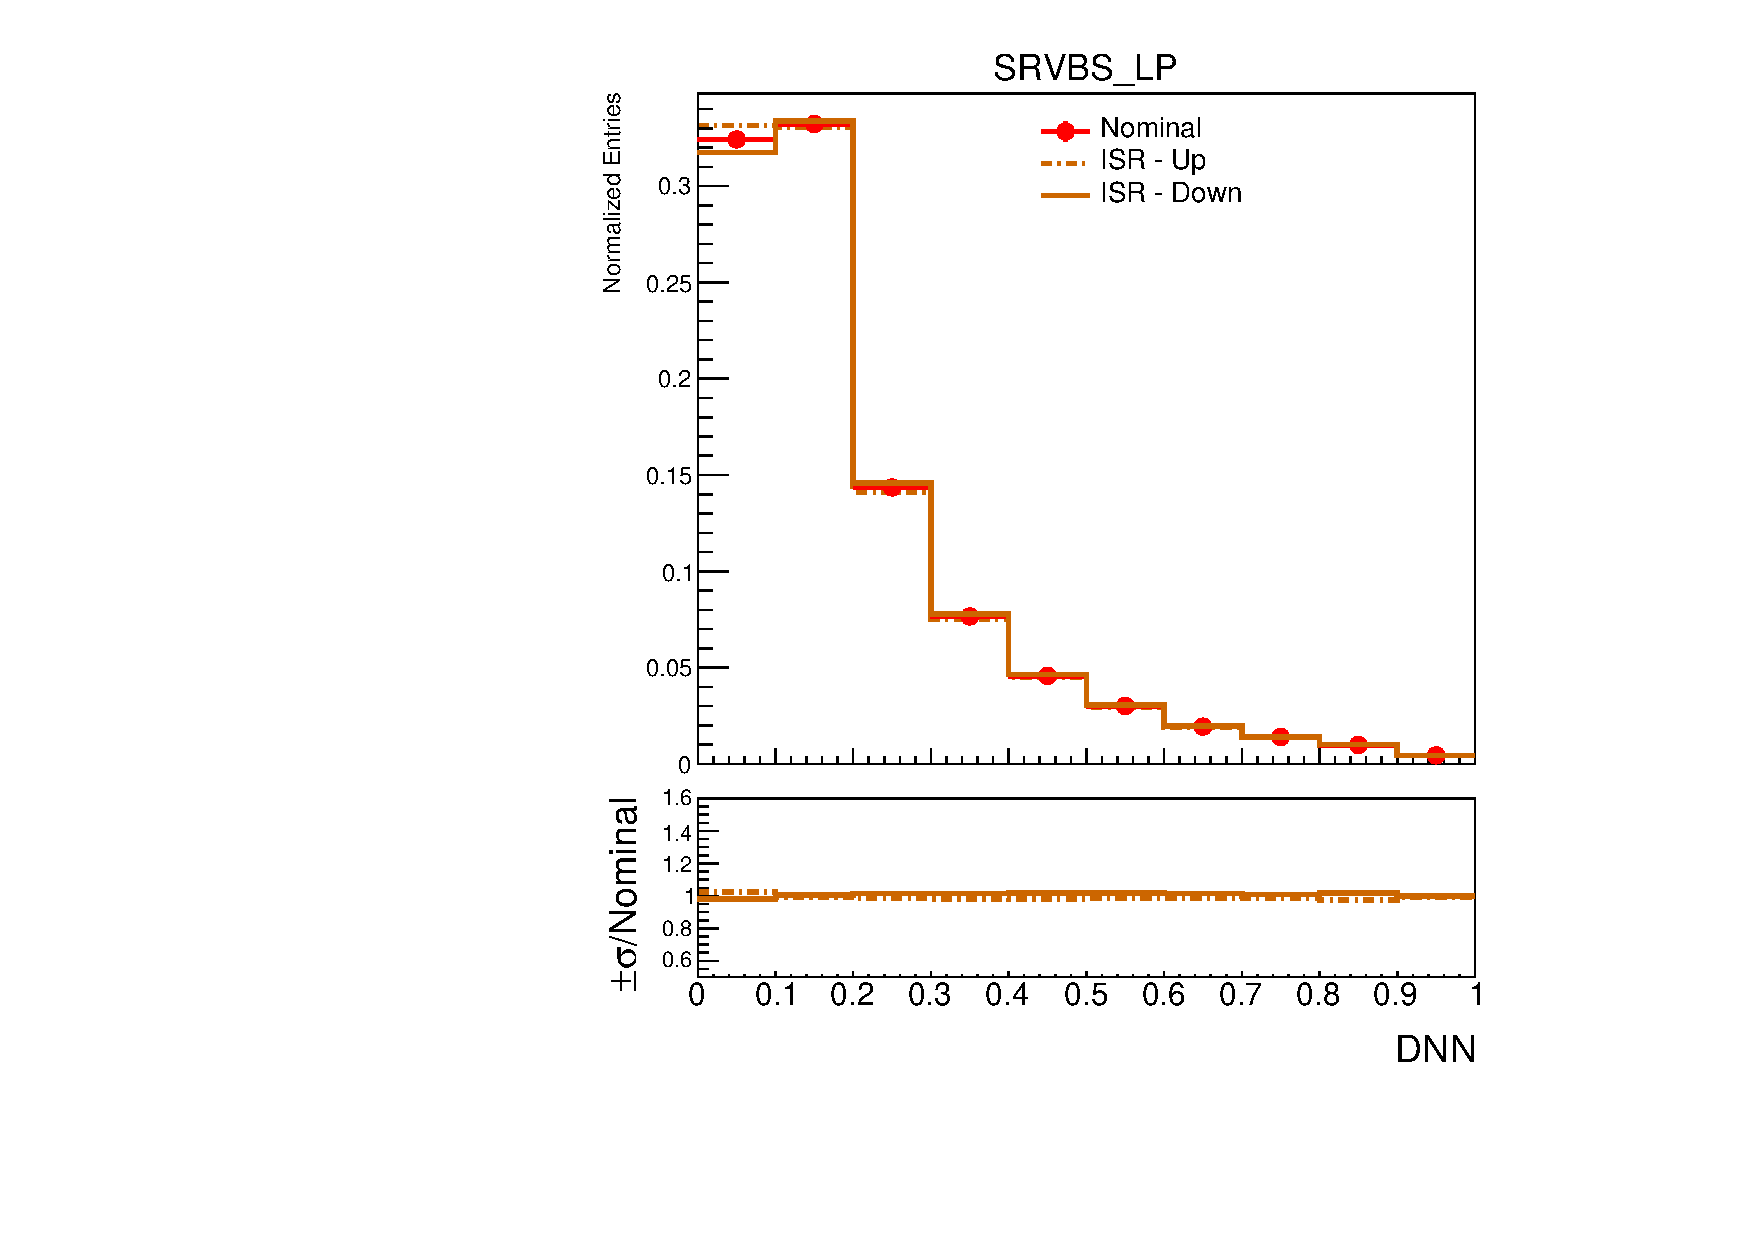
\includegraphics[width=\textwidth]{figures/1lep/PDFUnc/ISR/ttbar_0ptag1pfat0pjet_0ptv_SRVBS_LP_DNN_SysTheoryISR_ttbar__1up_Norm.pdf}
        \caption{\ttbar, merged LP SR}
    \end{subfigure}
    \\
    \vspace{5mm}
    \begin{subfigure}[b]{0.3\textwidth}
        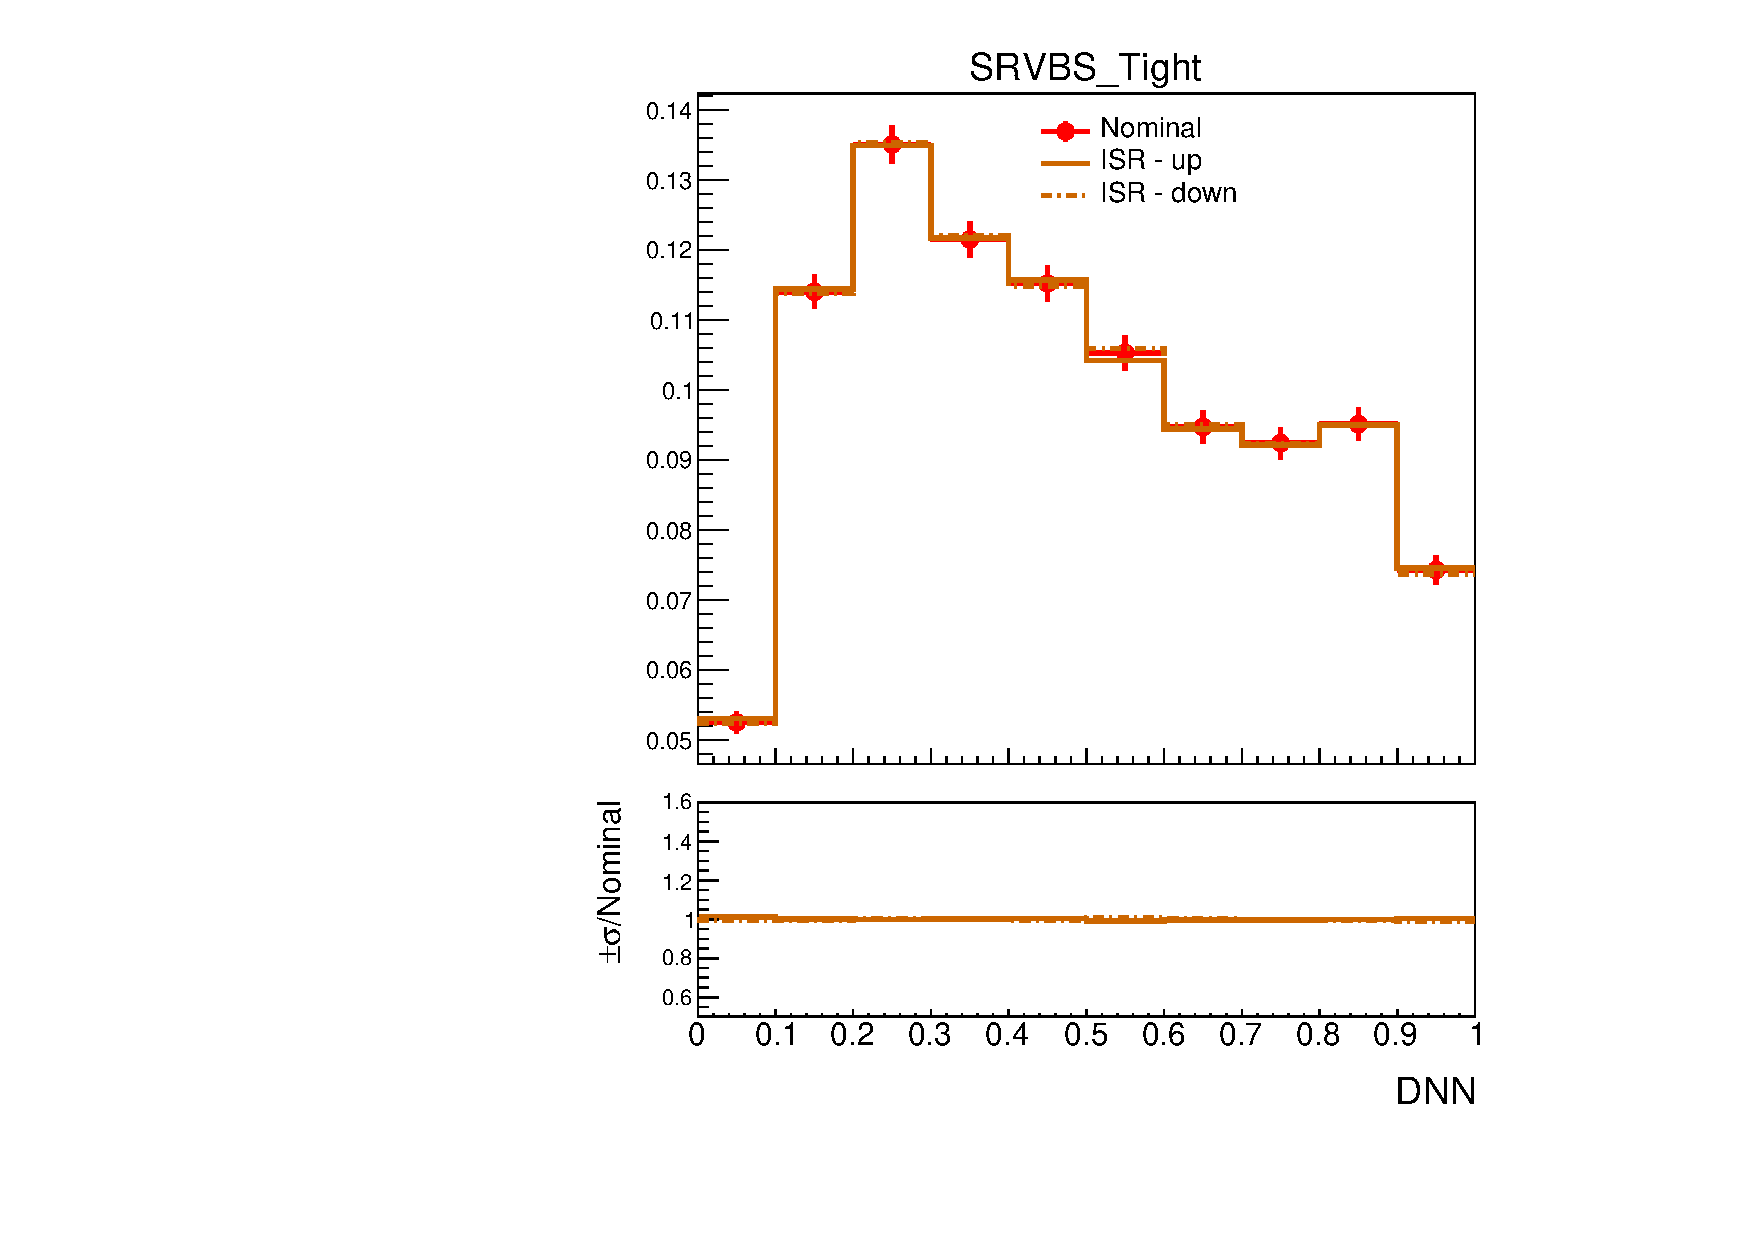
\includegraphics[width=\textwidth]{figures/1lep/PDFUnc/ISR/stop_0ptag2pjet_0ptv_SRVBS_Tight_DNN_SysTheoryISR_stop__1up_Norm.pdf}
        \caption{single top, resolved SR}
    \end{subfigure}
    \begin{subfigure}[b]{0.3\textwidth}
        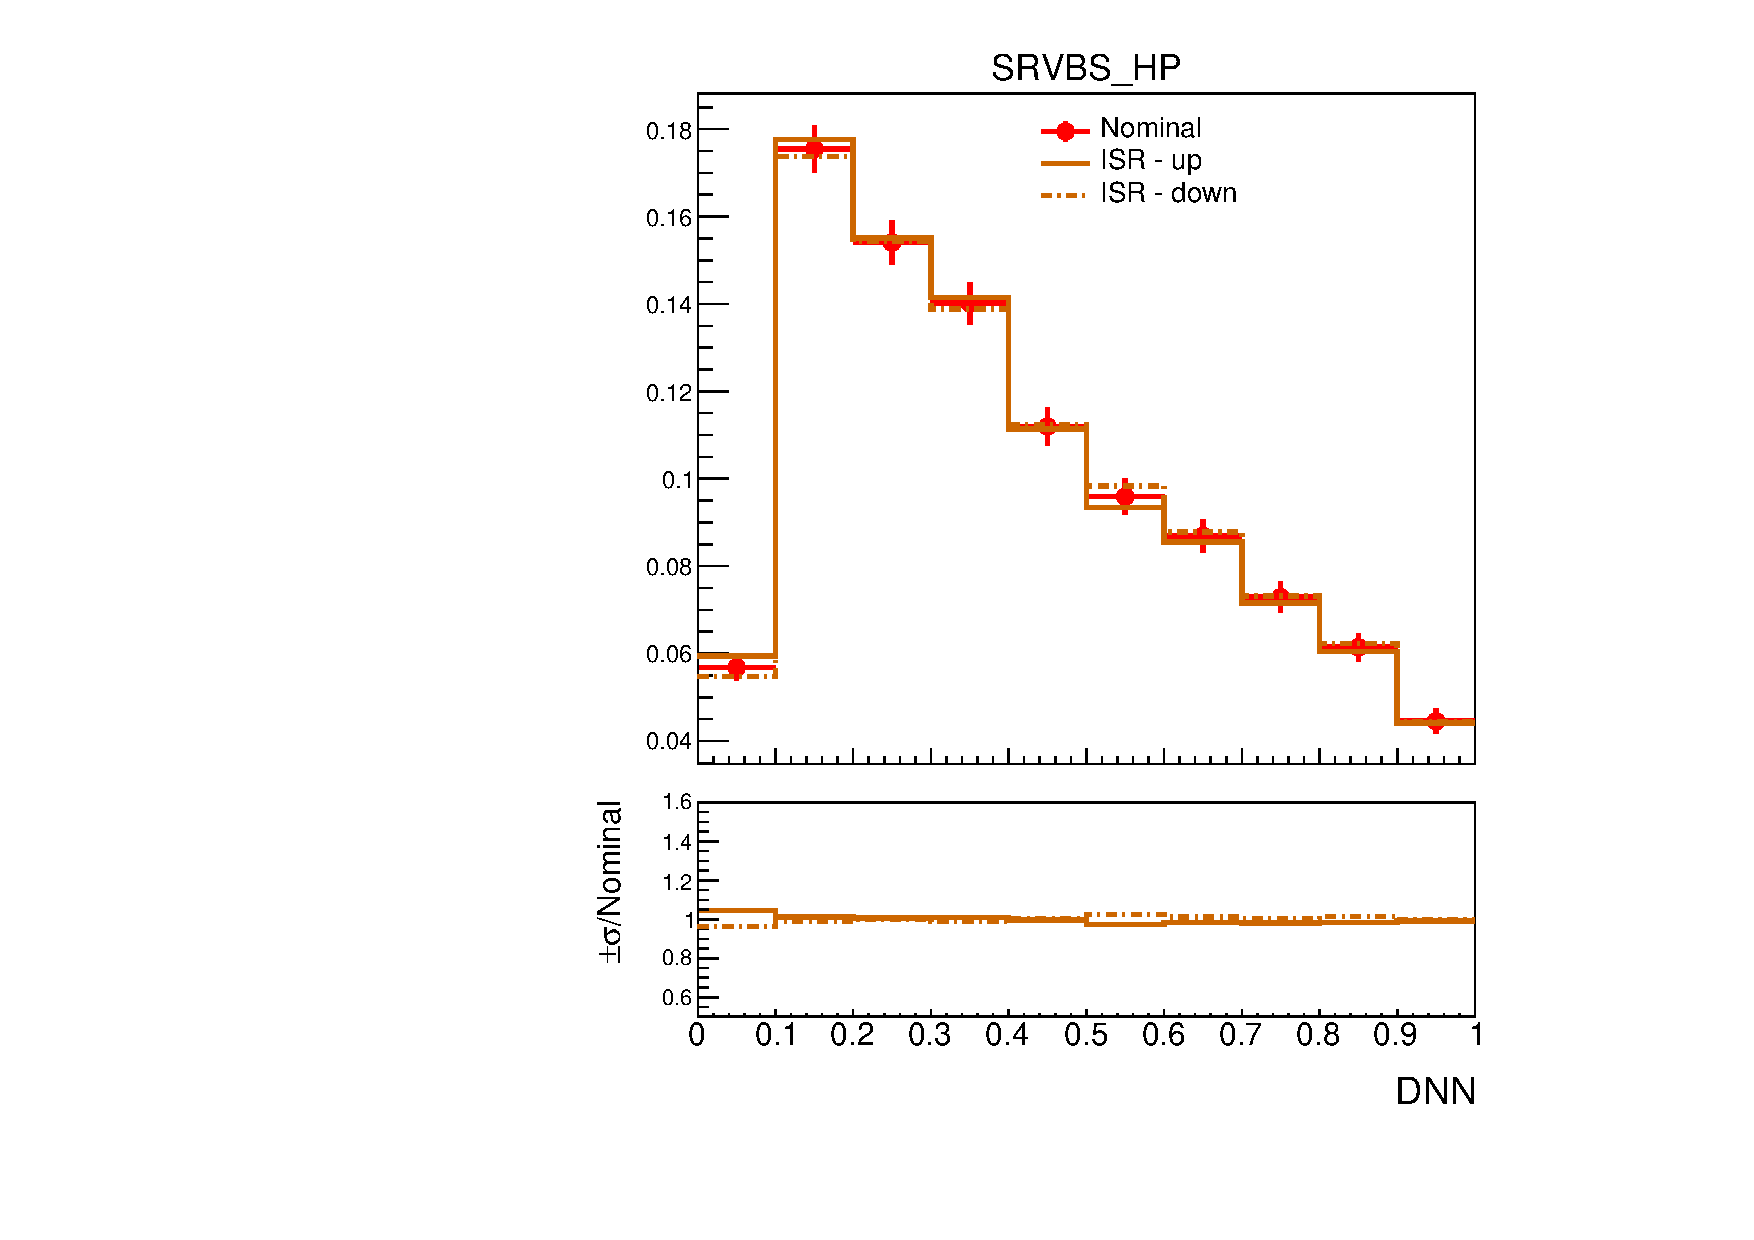
\includegraphics[width=\textwidth]{figures/1lep/PDFUnc/ISR/stop_0ptag1pfat0pjet_0ptv_SRVBS_HP_DNN_SysTheoryISR_stop__1up_Norm.pdf}
        \caption{single top, merged HP SR}
    \end{subfigure}
    \begin{subfigure}[b]{0.3\textwidth}
        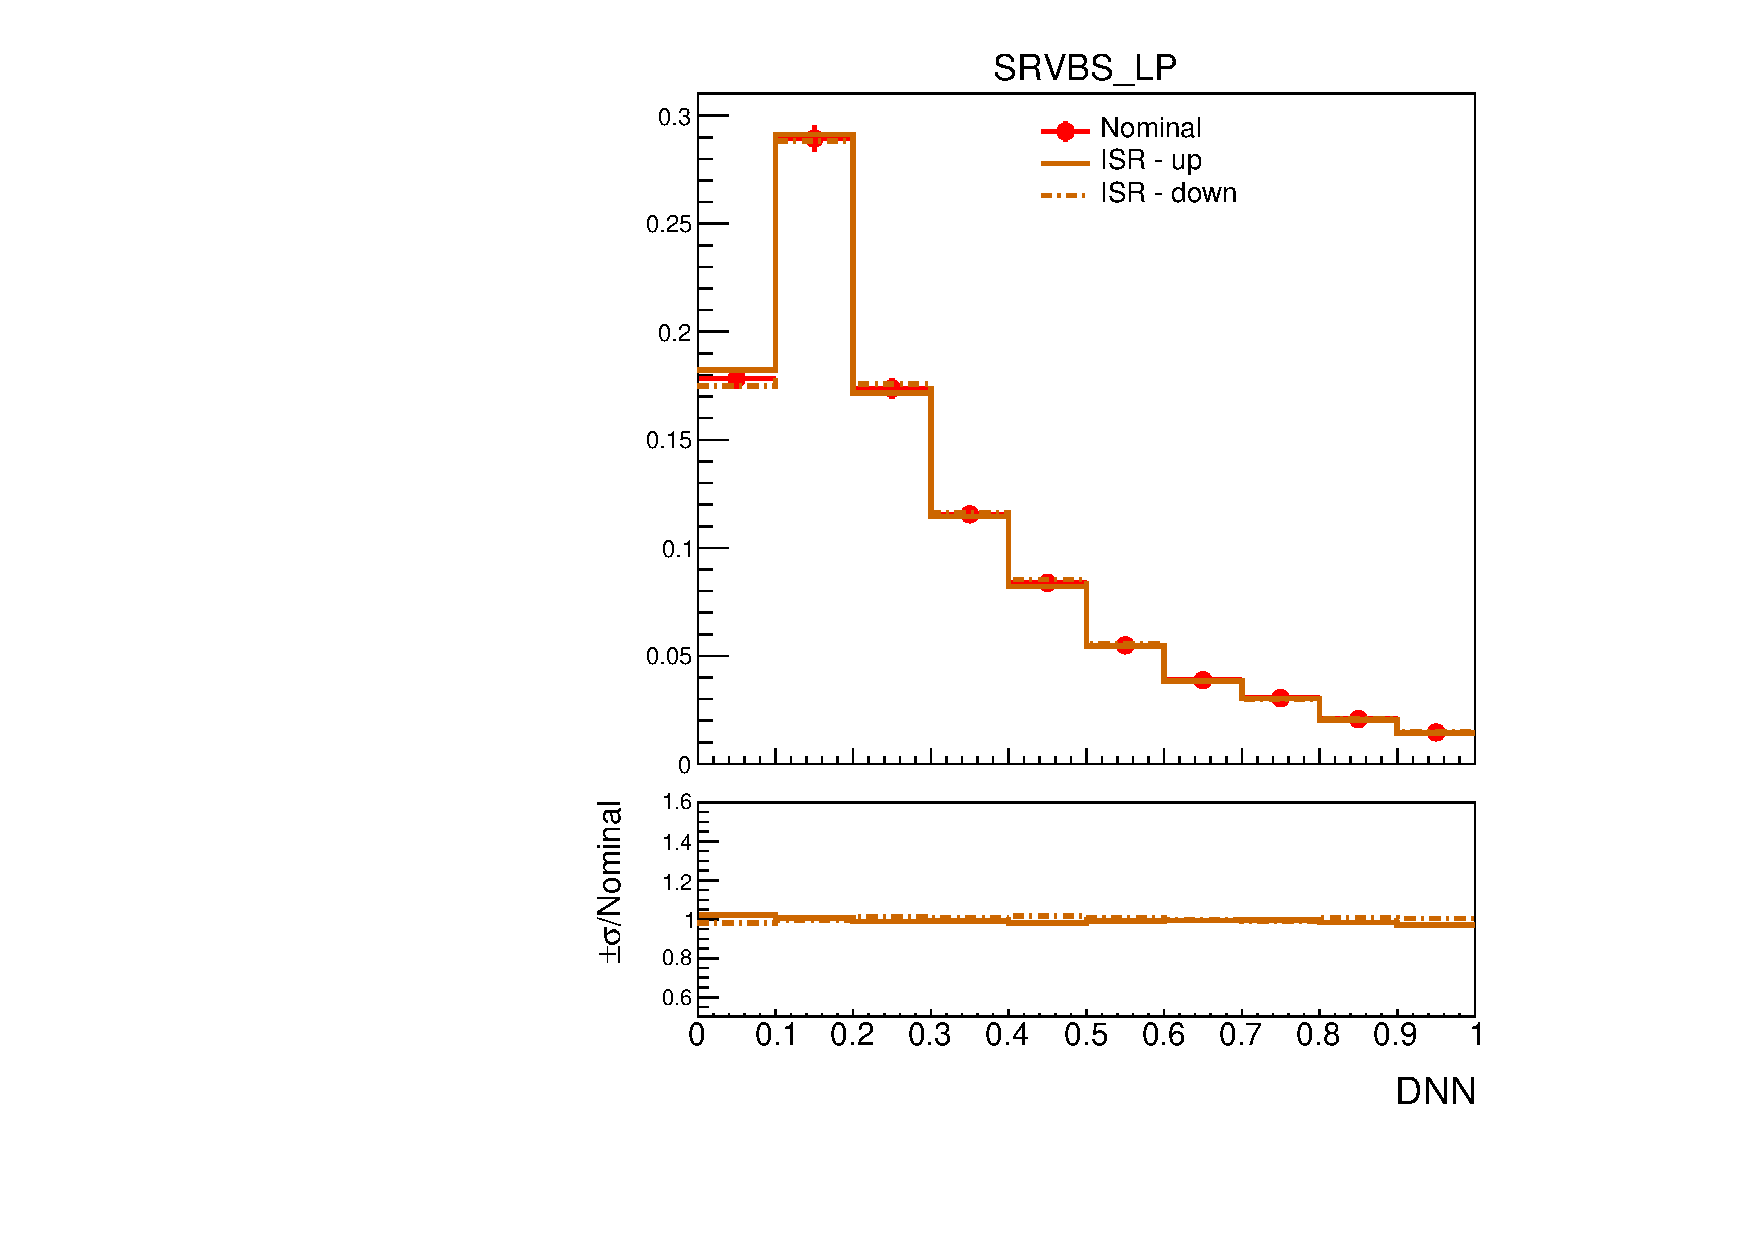
\includegraphics[width=\textwidth]{figures/1lep/PDFUnc/ISR/stop_0ptag1pfat0pjet_0ptv_SRVBS_LP_DNN_SysTheoryISR_stop__1up_Norm.pdf}
        \caption{single top, merged LP SR}
    \end{subfigure}
%%%    \\
%%%    \vspace{5mm}
%%%    \begin{subfigure}[b]{0.3\textwidth}
%%%        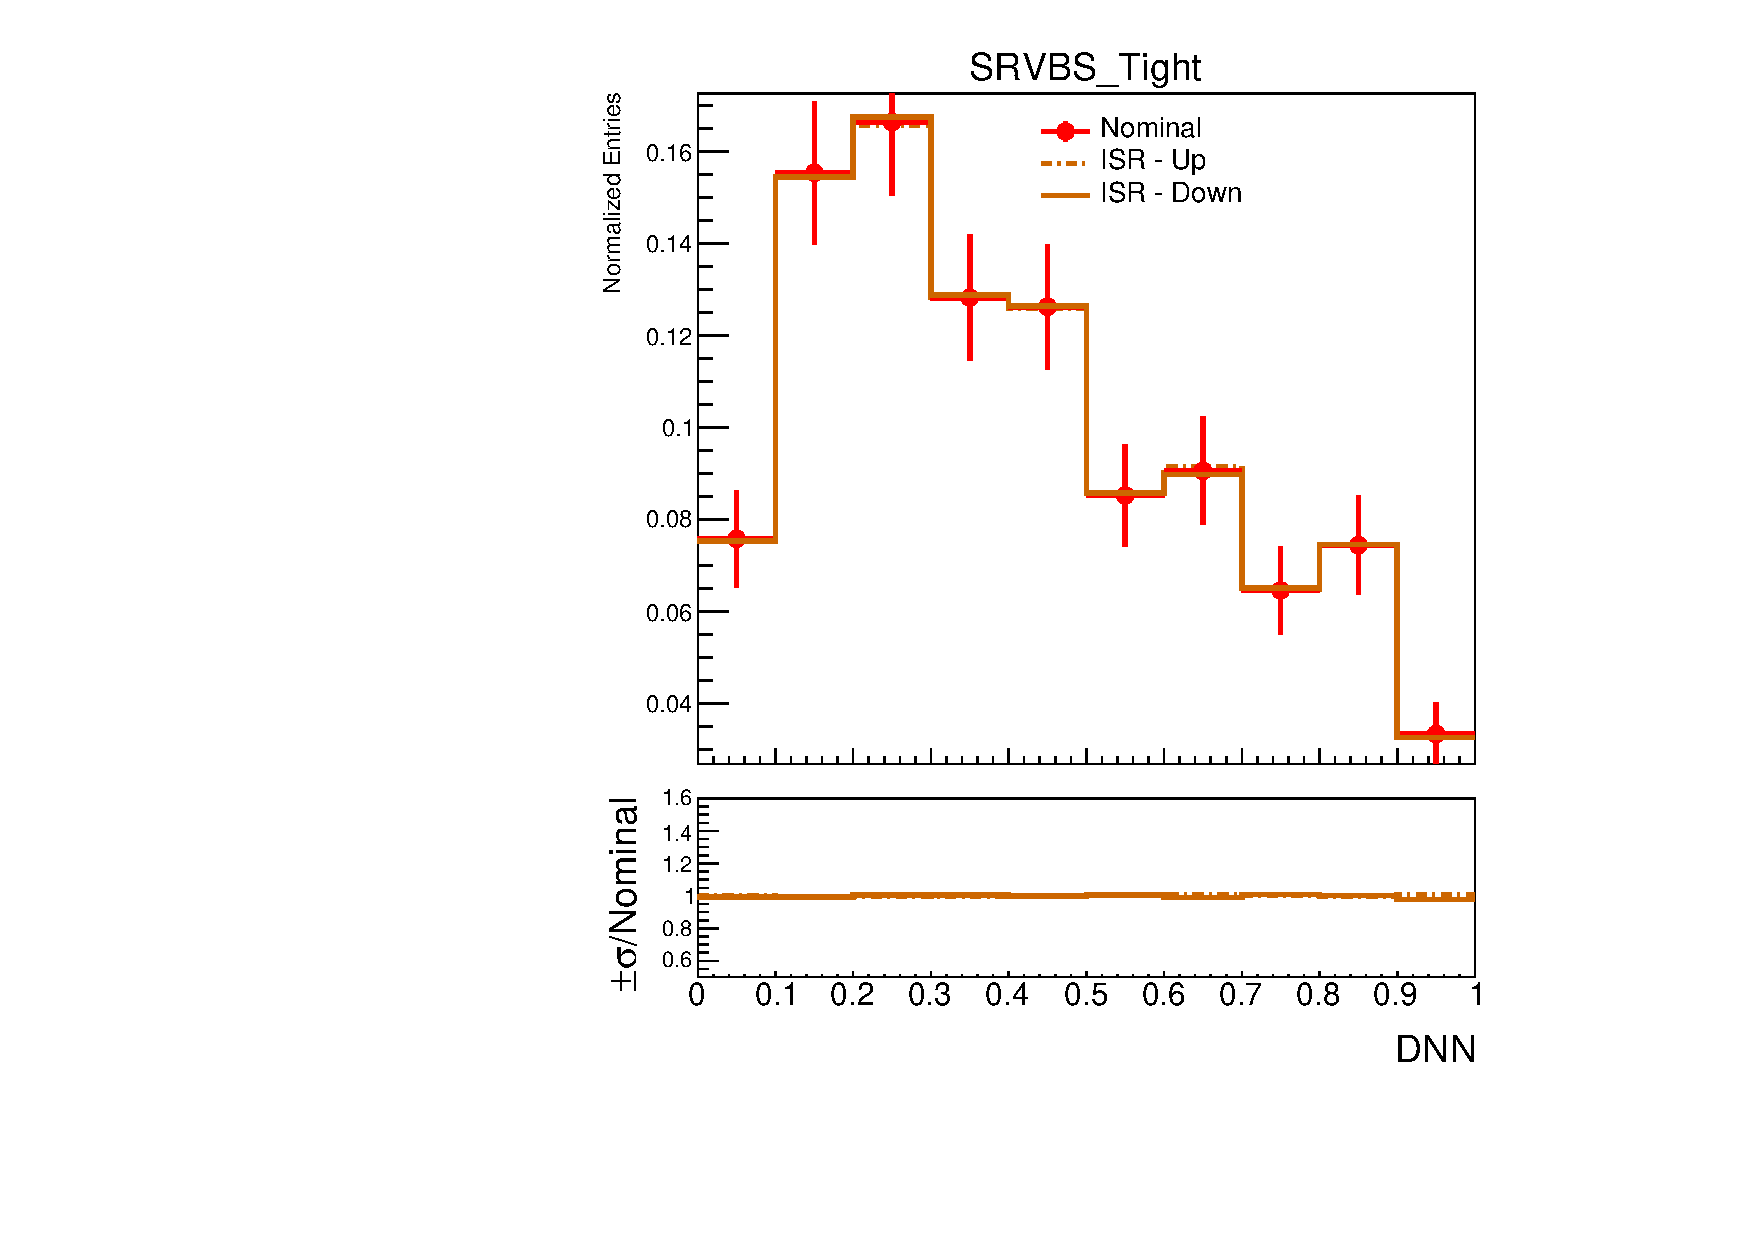
\includegraphics[width=\textwidth]{figures/1lep/PDFUnc/ISR/stops_0ptag2pjet_0ptv_SRVBS_Tight_DNN_SysTheoryISR_stop__1up_Norm.pdf}
%%%        \caption{stops, resolved SR}
%%%    \end{subfigure}
%%%    \begin{subfigure}[b]{0.3\textwidth}
%%%        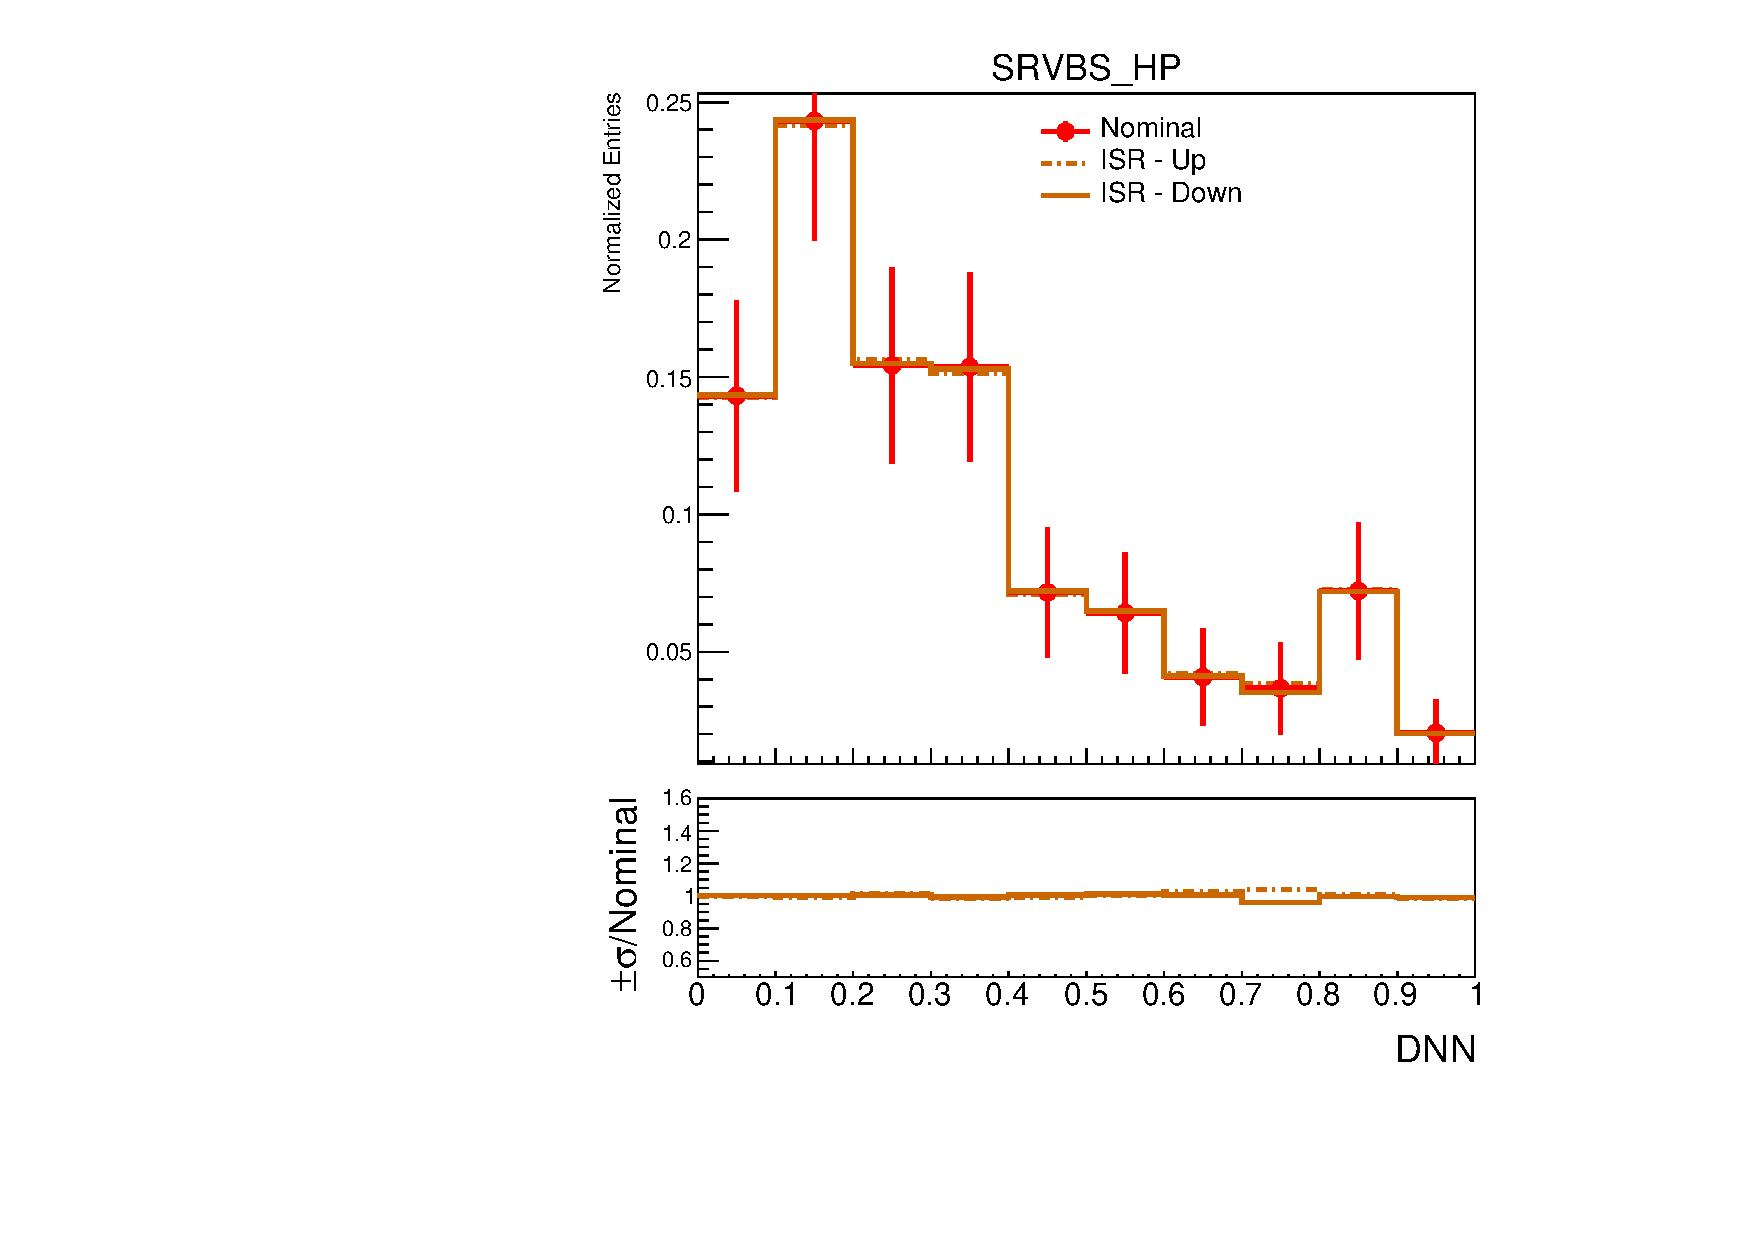
\includegraphics[width=\textwidth]{figures/1lep/PDFUnc/ISR/stops_0ptag1pfat0pjet_0ptv_SRVBS_HP_DNN_SysTheoryISR_stop__1up_Norm.pdf}
%%%        \caption{stops, merged HP SR}
%%%    \end{subfigure}
%%%    \begin{subfigure}[b]{0.3\textwidth}
%%%        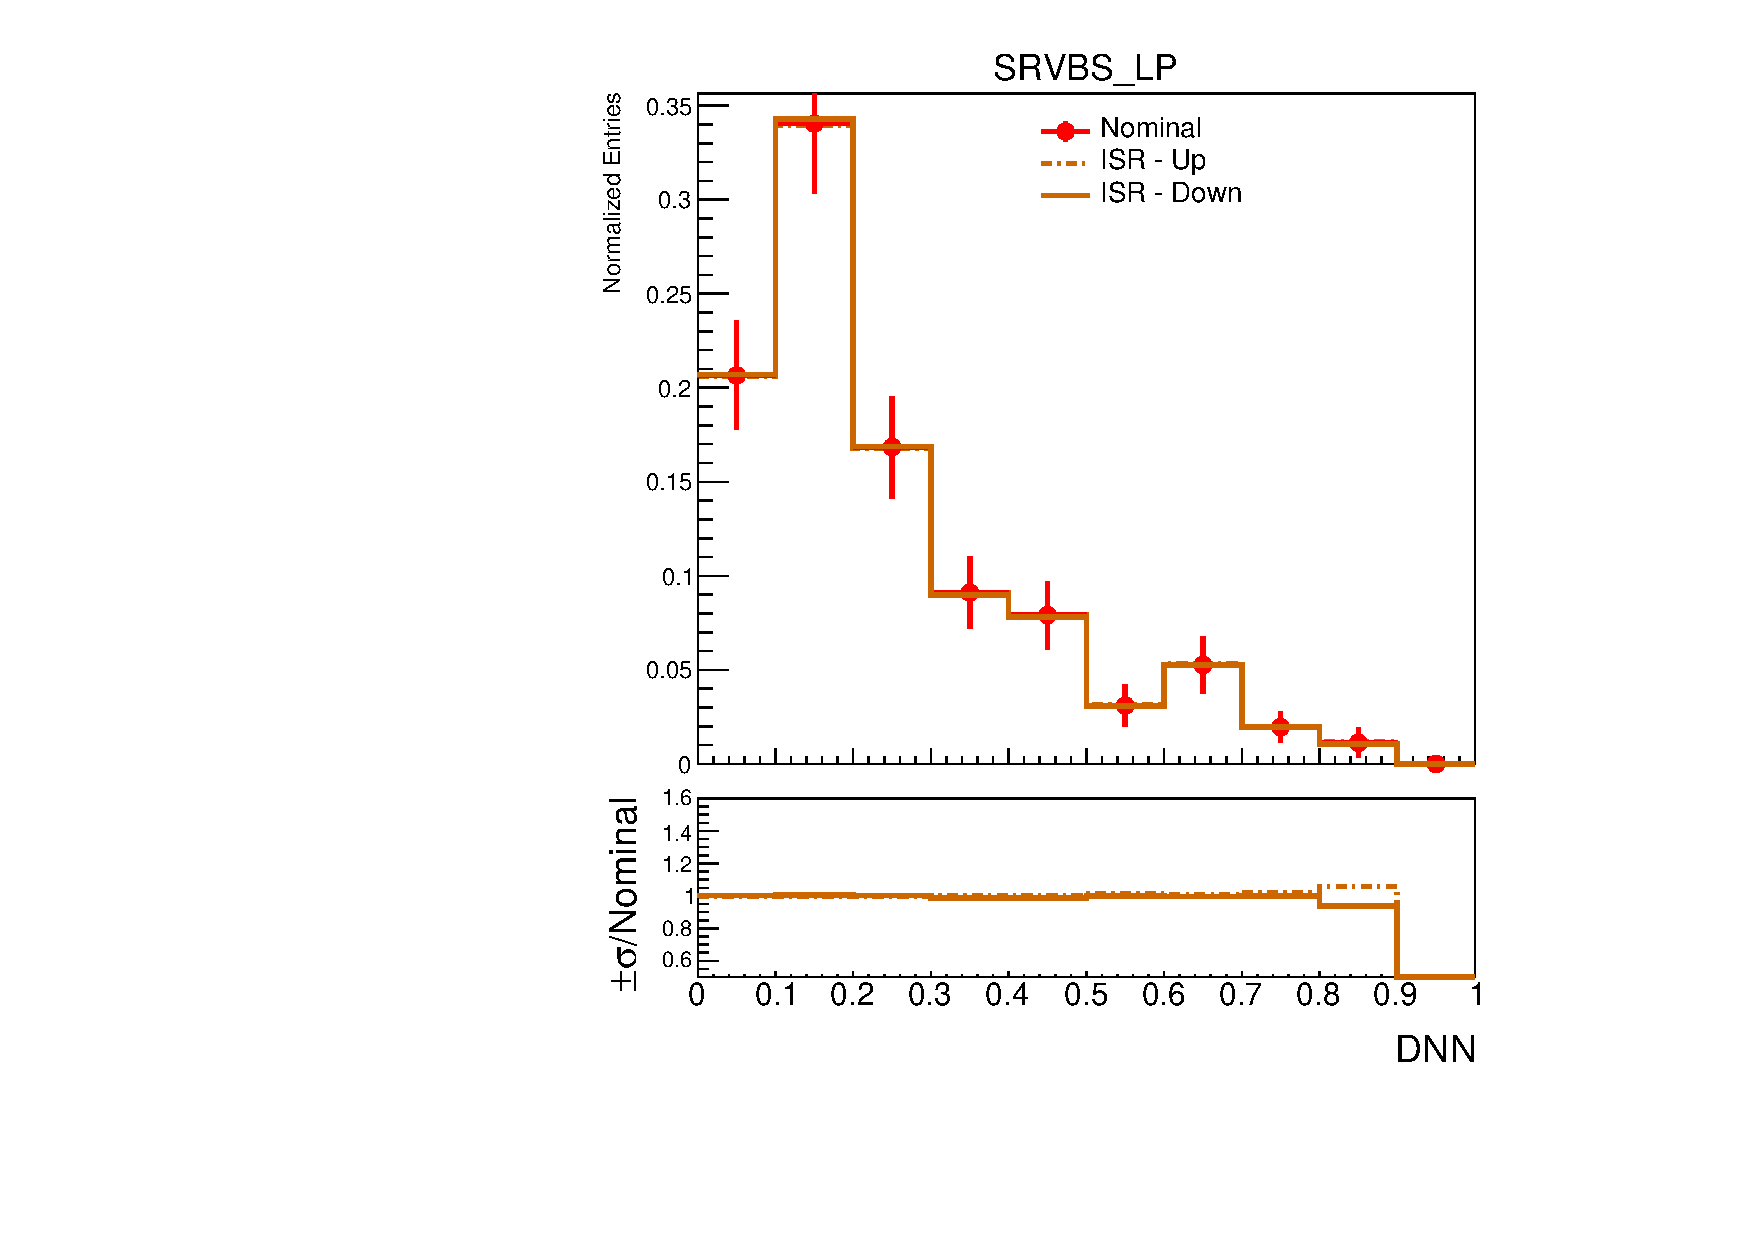
\includegraphics[width=\textwidth]{figures/1lep/PDFUnc/ISR/stops_0ptag1pfat0pjet_0ptv_SRVBS_LP_DNN_SysTheoryISR_stop__1up_Norm.pdf}
%%%        \caption{stops, merged LP SR}
%%%    \end{subfigure}
%%%    \\
%%%    \vspace{5mm}
%%%    \begin{subfigure}[b]{0.3\textwidth}
%%%        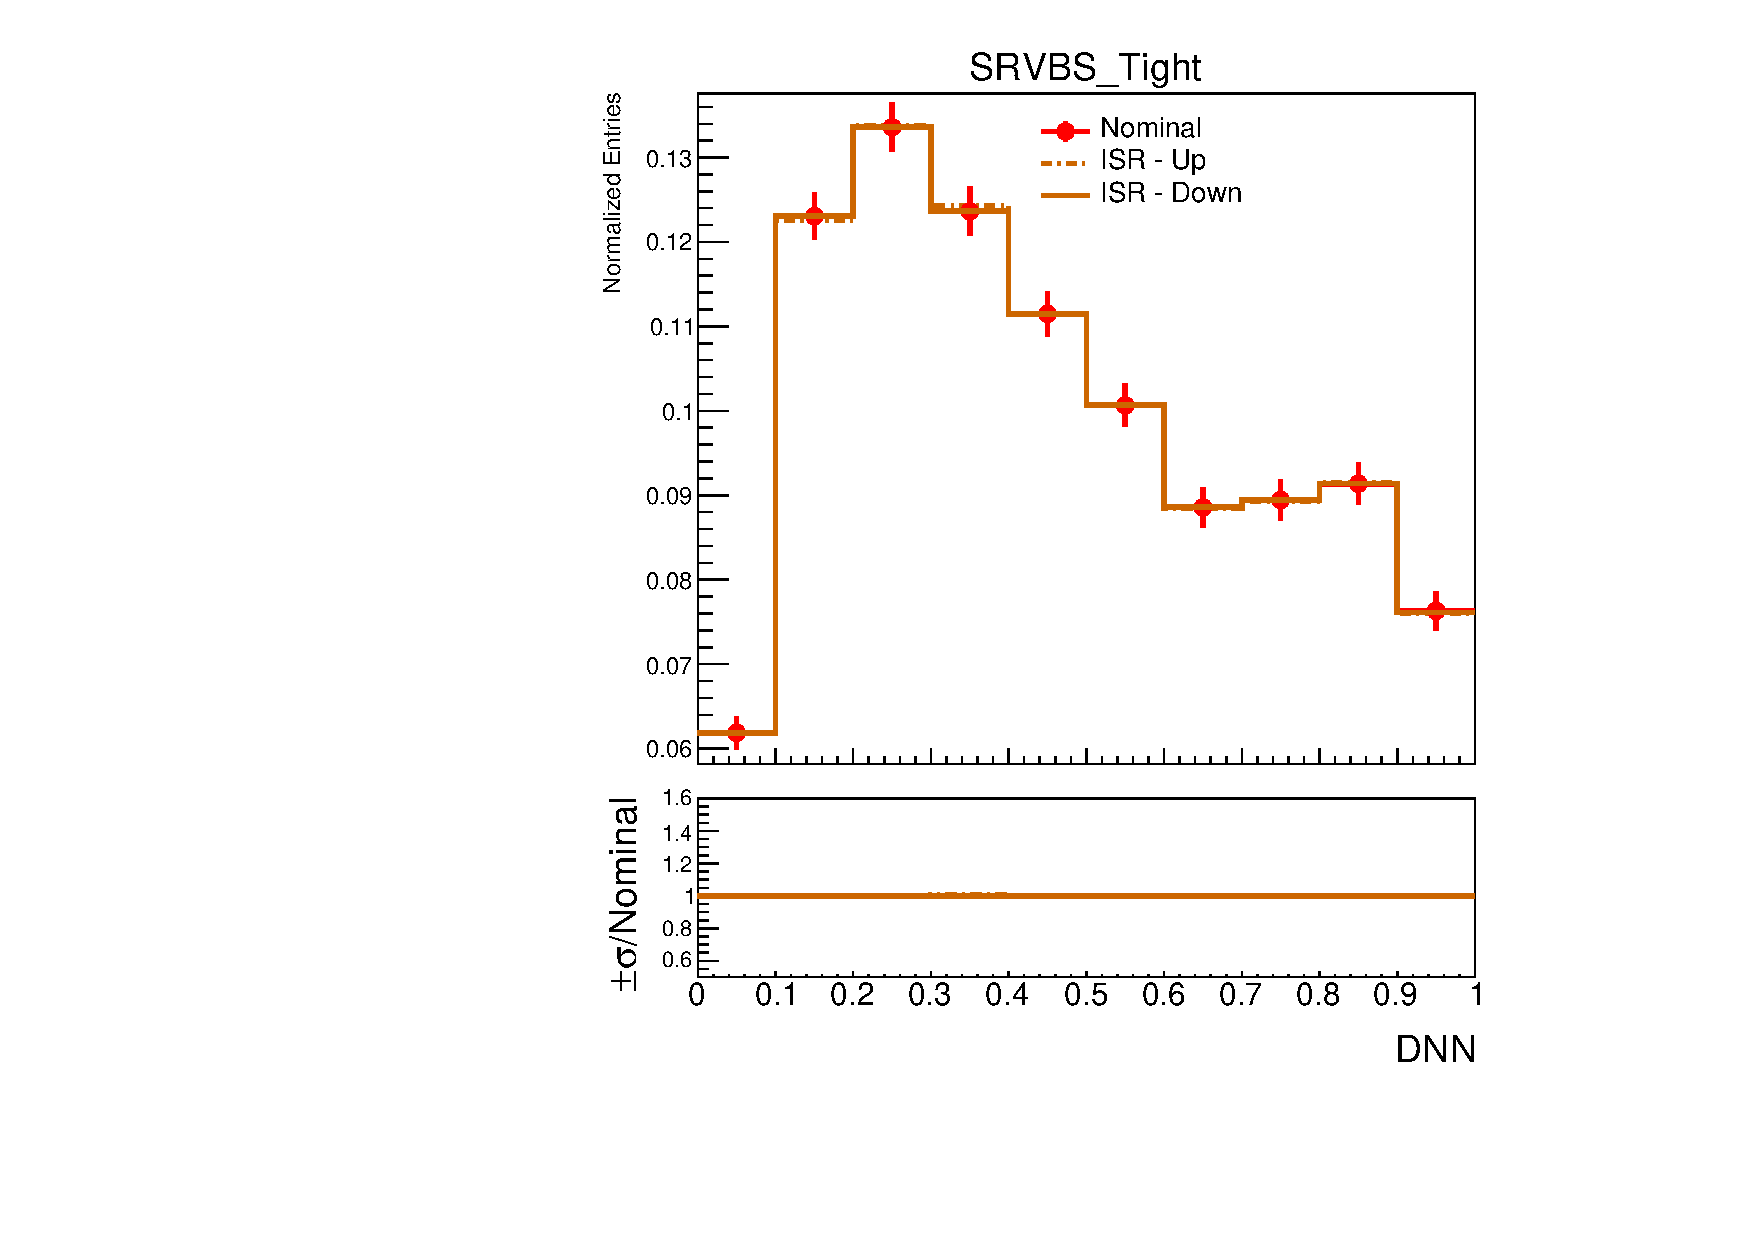
\includegraphics[width=\textwidth]{figures/1lep/PDFUnc/ISR/stopt_0ptag2pjet_0ptv_SRVBS_Tight_DNN_SysTheoryISR_stop__1up_Norm.pdf}
%%%        \caption{stopt, resolved SR}
%%%    \end{subfigure}
%%%    \begin{subfigure}[b]{0.3\textwidth}
%%%        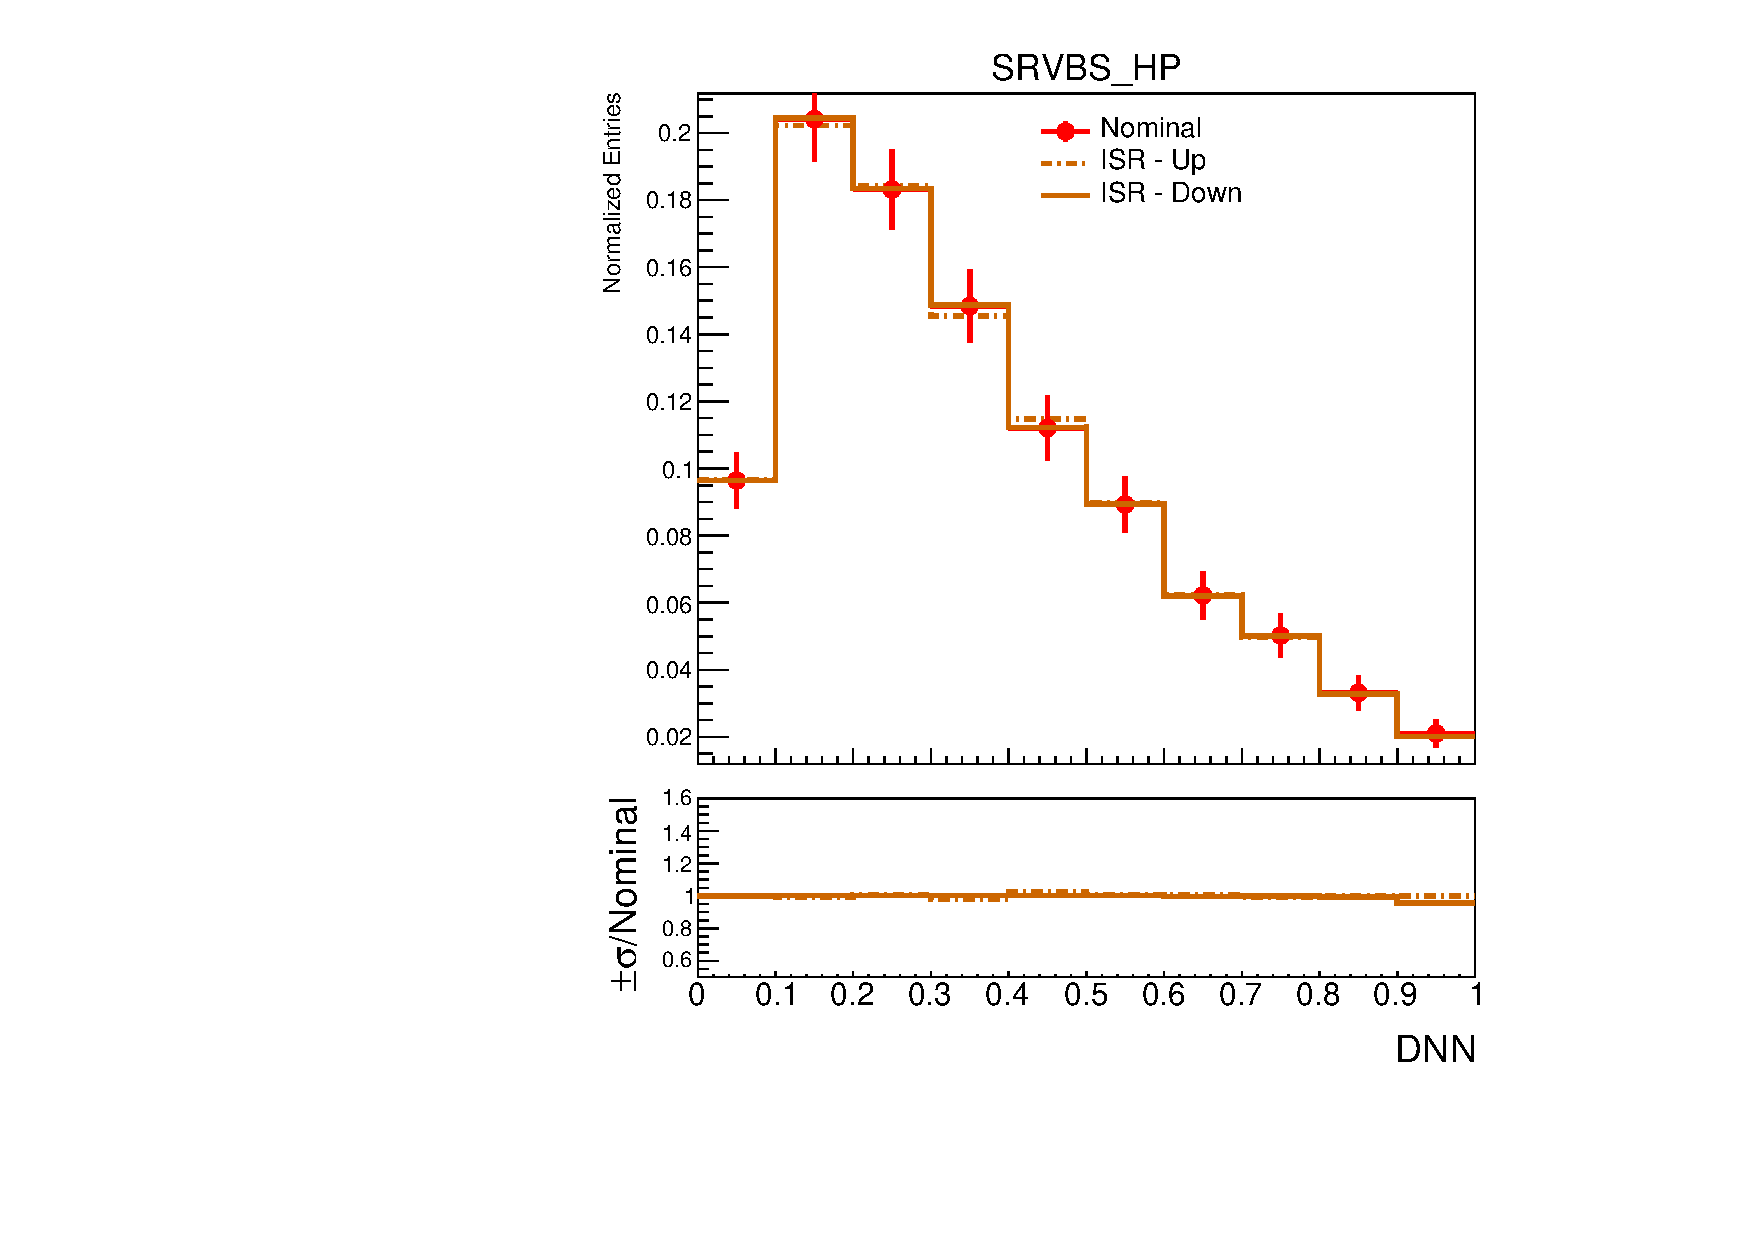
\includegraphics[width=\textwidth]{figures/1lep/PDFUnc/ISR/stopt_0ptag1pfat0pjet_0ptv_SRVBS_HP_DNN_SysTheoryISR_stop__1up_Norm.pdf}
%%%        \caption{stopt, merged HP SR}
%%%    \end{subfigure}
%%%    \begin{subfigure}[b]{0.3\textwidth}
%%%        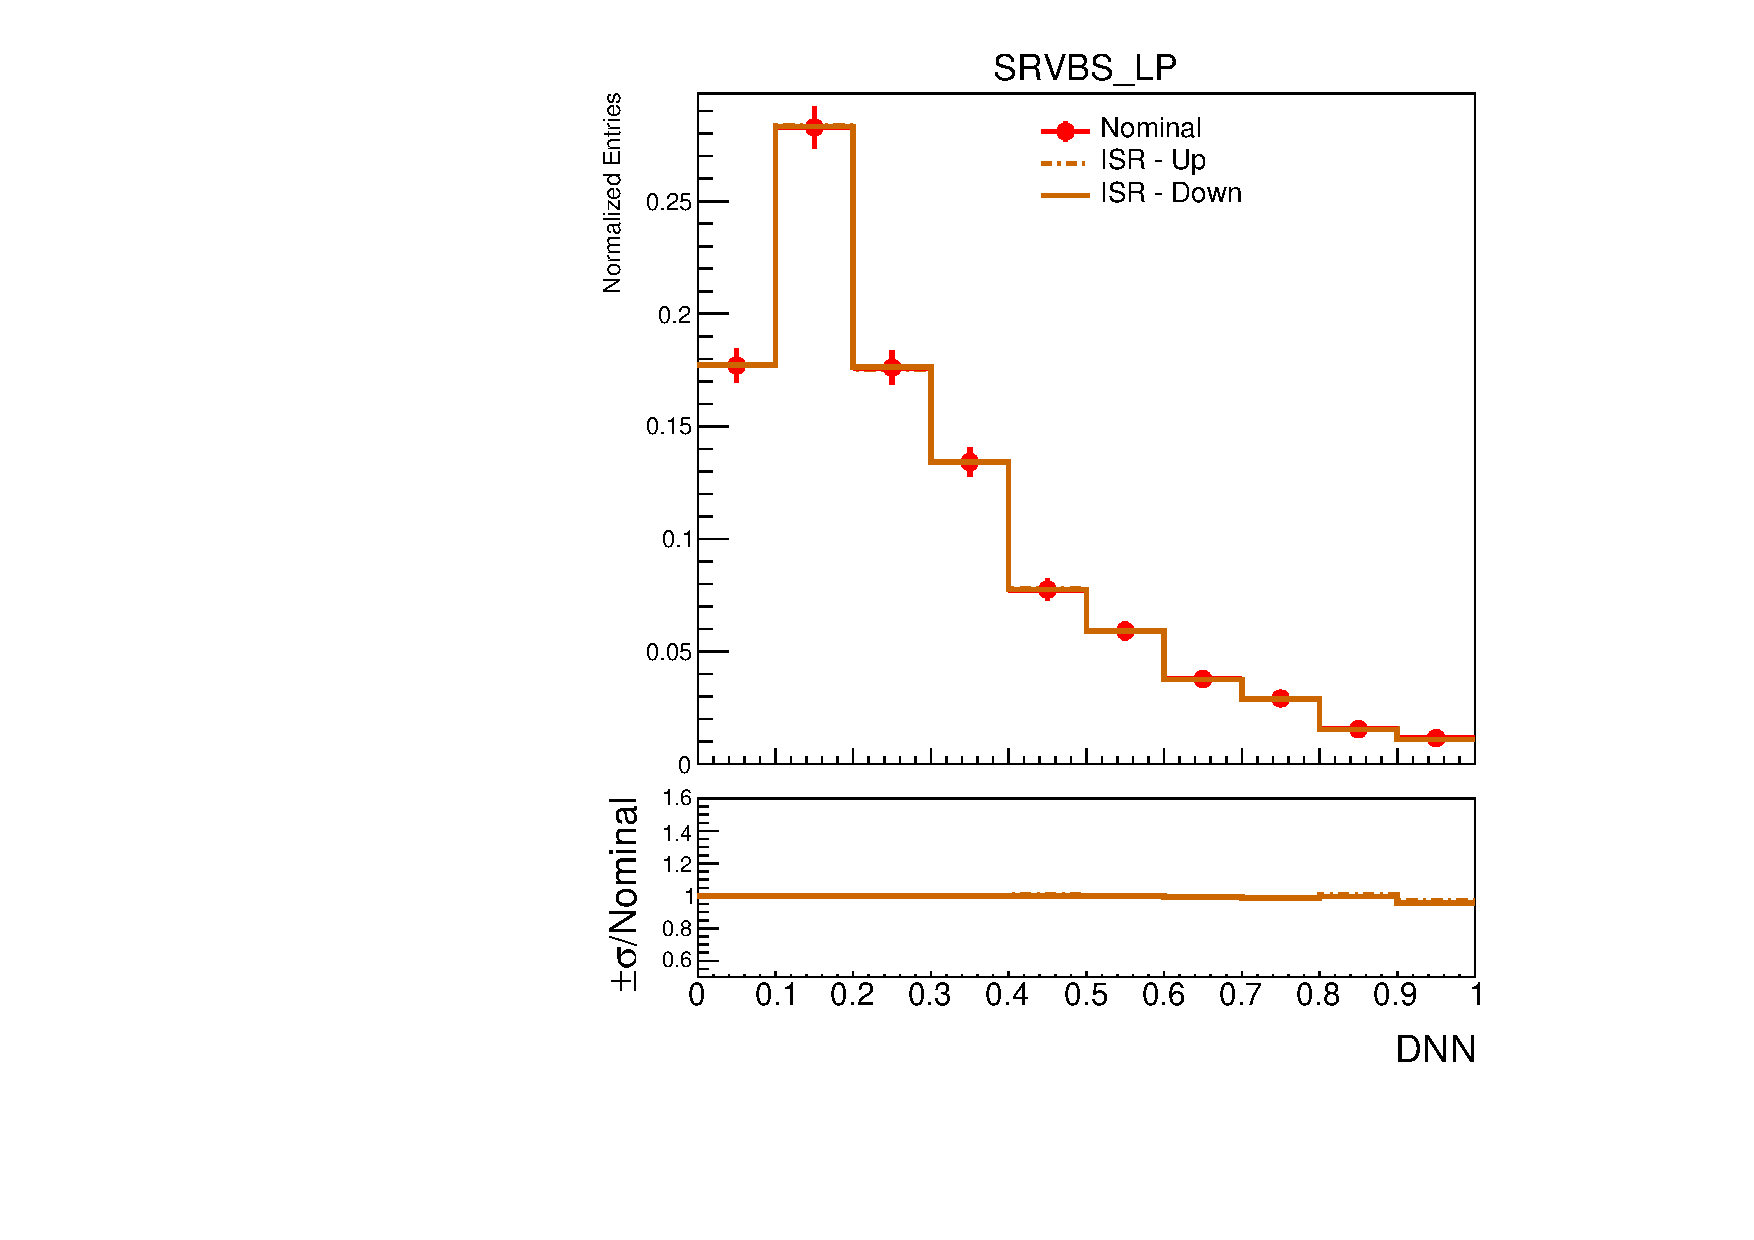
\includegraphics[width=\textwidth]{figures/1lep/PDFUnc/ISR/stopt_0ptag1pfat0pjet_0ptv_SRVBS_LP_DNN_SysTheoryISR_stop__1up_Norm.pdf}
%%%        \caption{stopt, merged LP SR}
%%%    \end{subfigure}
%%%    \\
%%%    \vspace{5mm}
%%%    \begin{subfigure}[b]{0.3\textwidth}
%%%        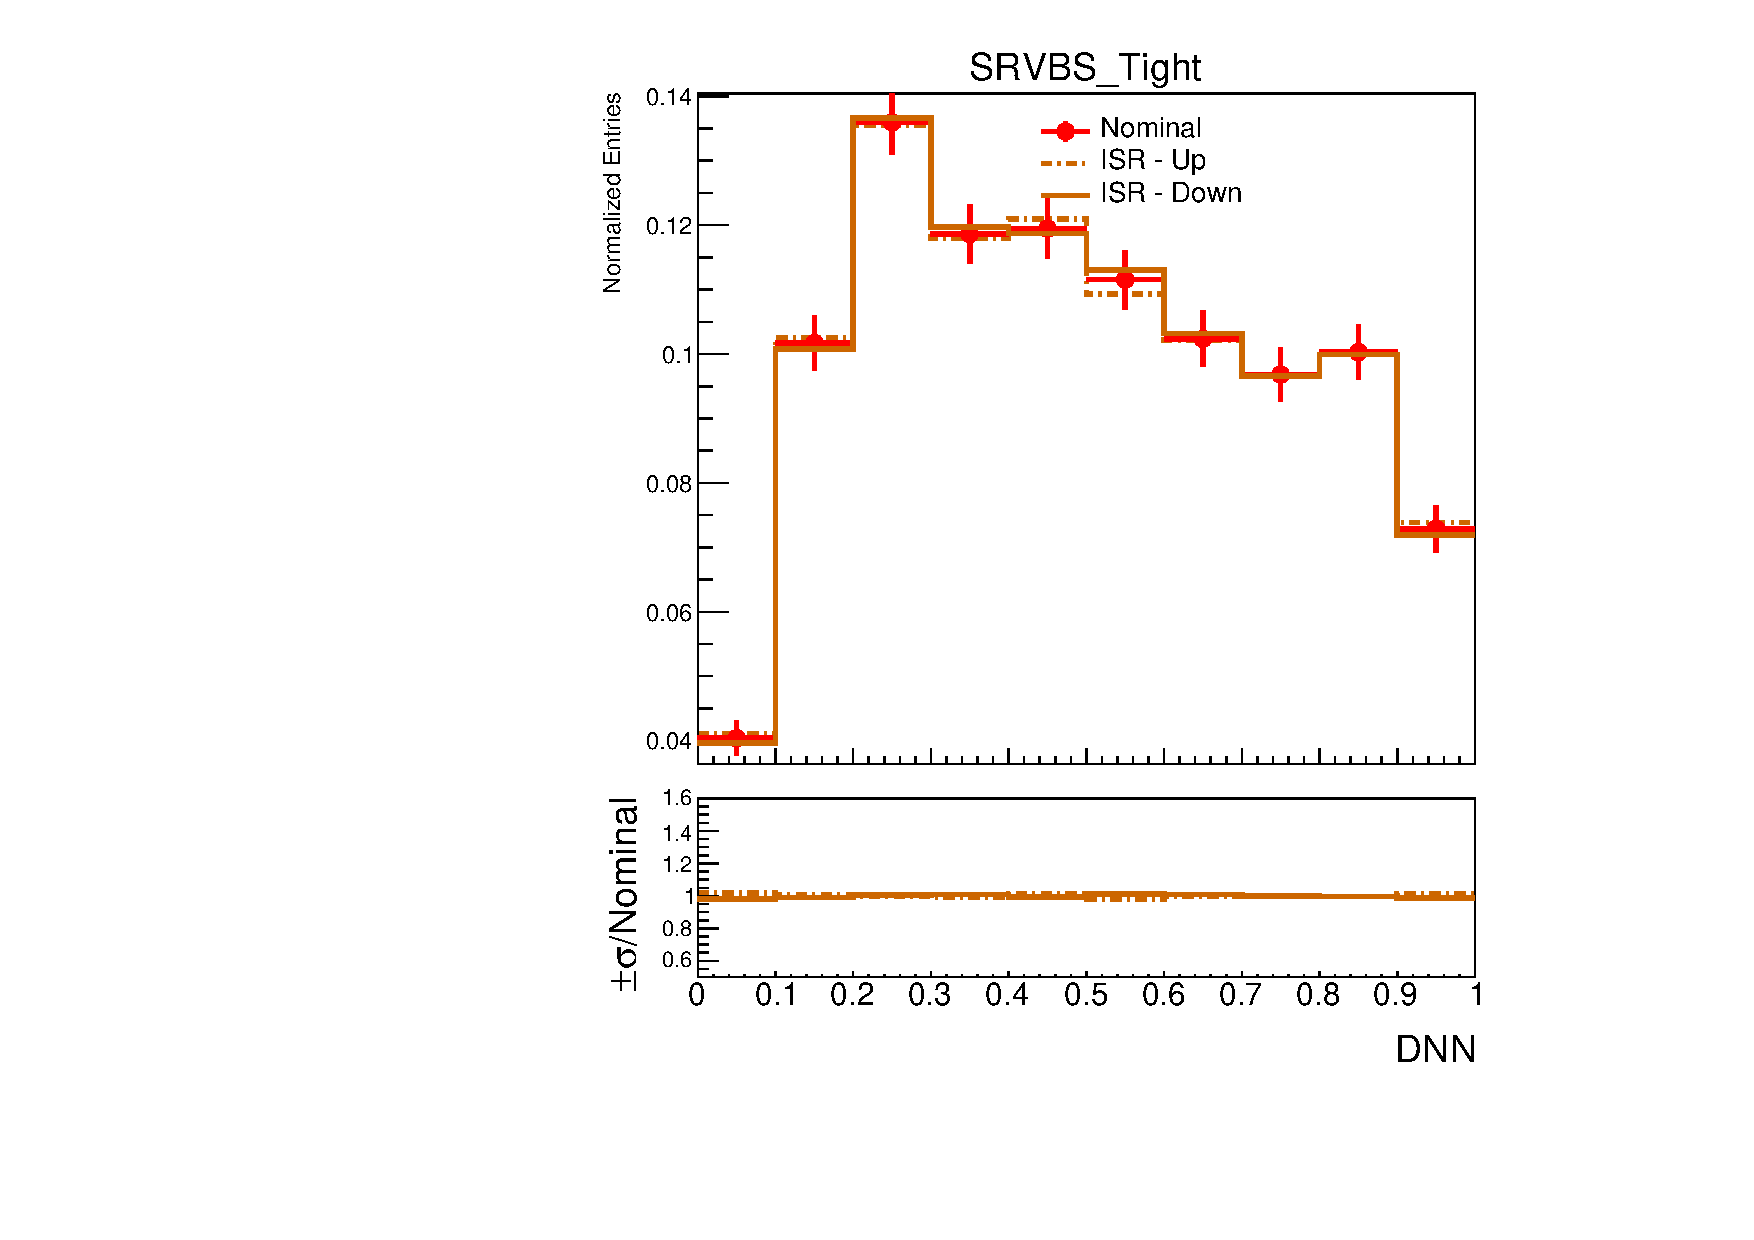
\includegraphics[width=\textwidth]{figures/1lep/PDFUnc/ISR/stopWt_0ptag2pjet_0ptv_SRVBS_Tight_DNN_SysTheoryISR_stop__1up_Norm.pdf}
%%%        \caption{stopWt, resolved SR}
%%%    \end{subfigure}
%%%    \begin{subfigure}[b]{0.3\textwidth}
%%%        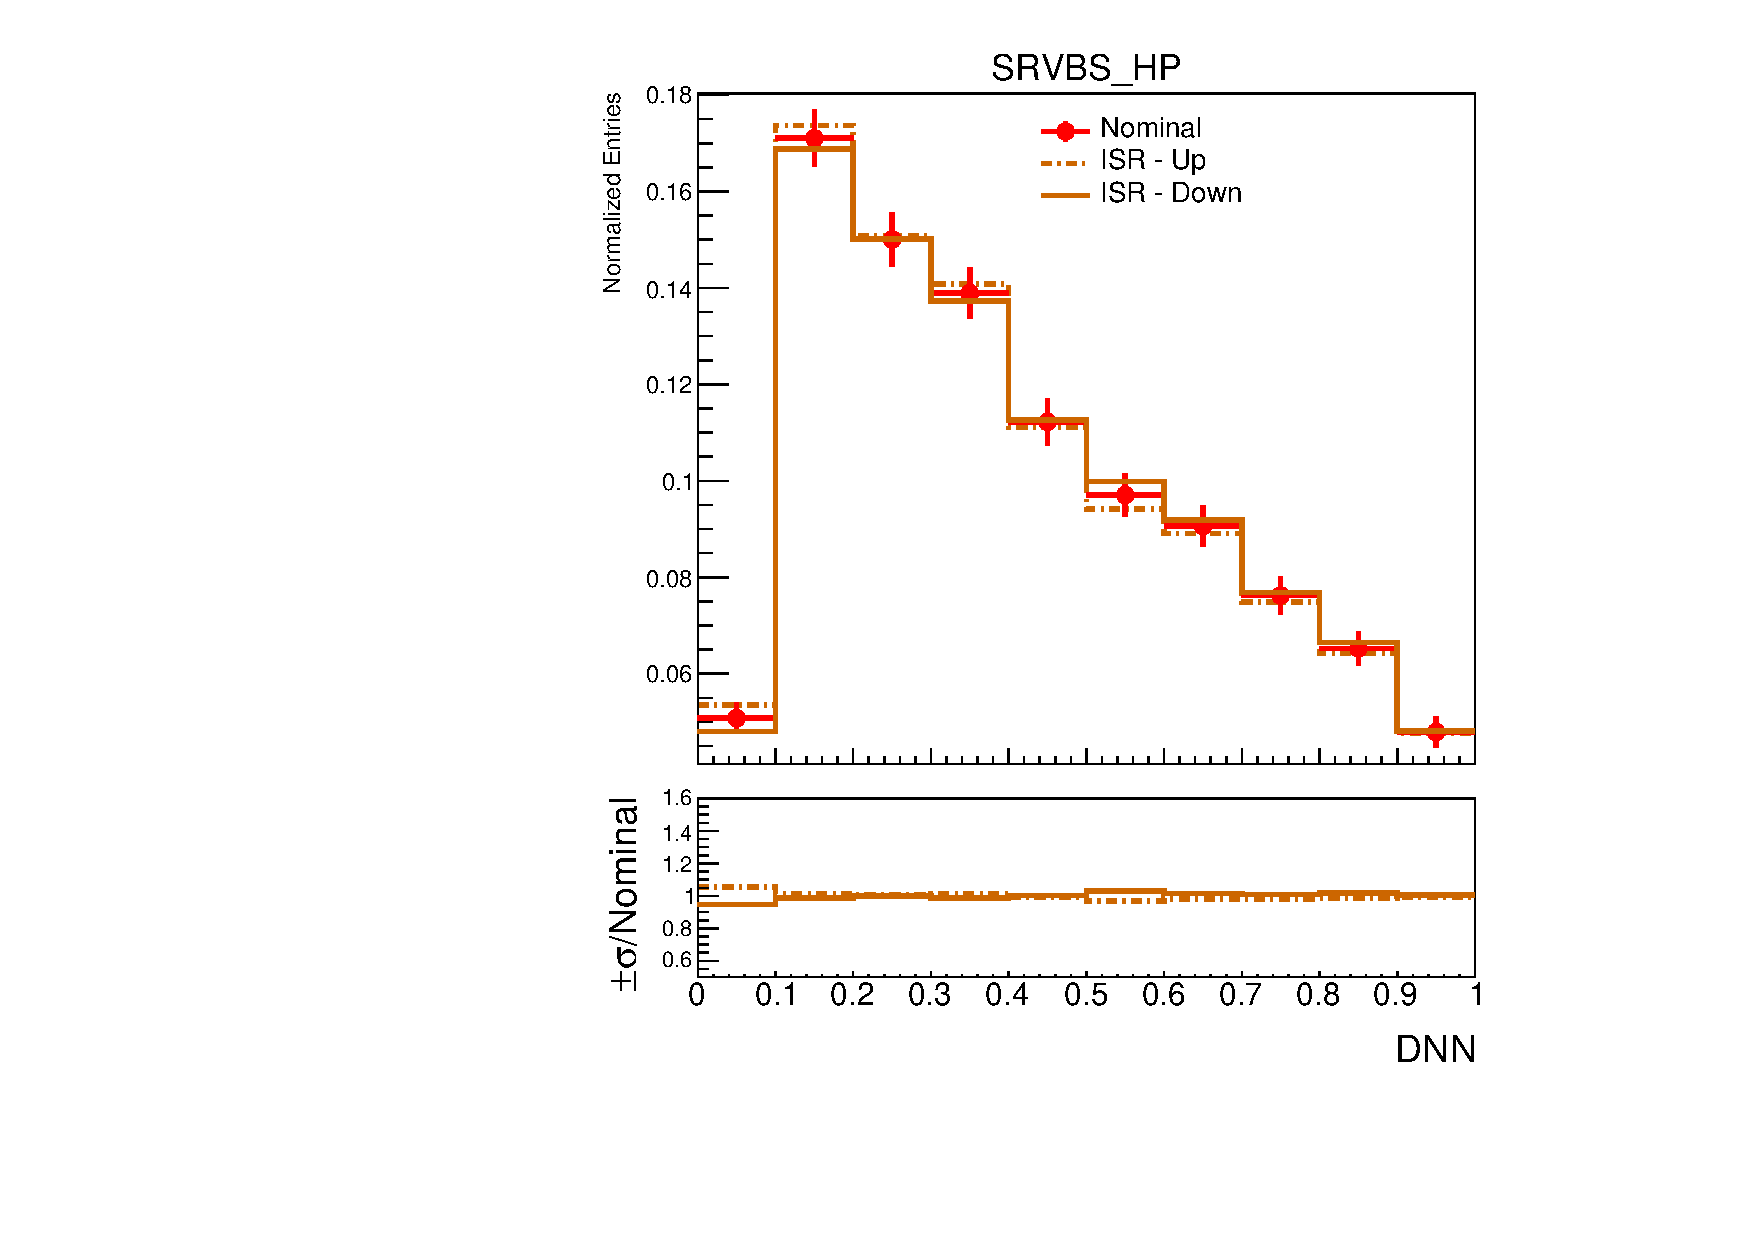
\includegraphics[width=\textwidth]{figures/1lep/PDFUnc/ISR/stopWt_0ptag1pfat0pjet_0ptv_SRVBS_HP_DNN_SysTheoryISR_stop__1up_Norm.pdf}
%%%        \caption{stopWt, merged HP SR}
%%%    \end{subfigure}
%%%    \begin{subfigure}[b]{0.3\textwidth}
%%%        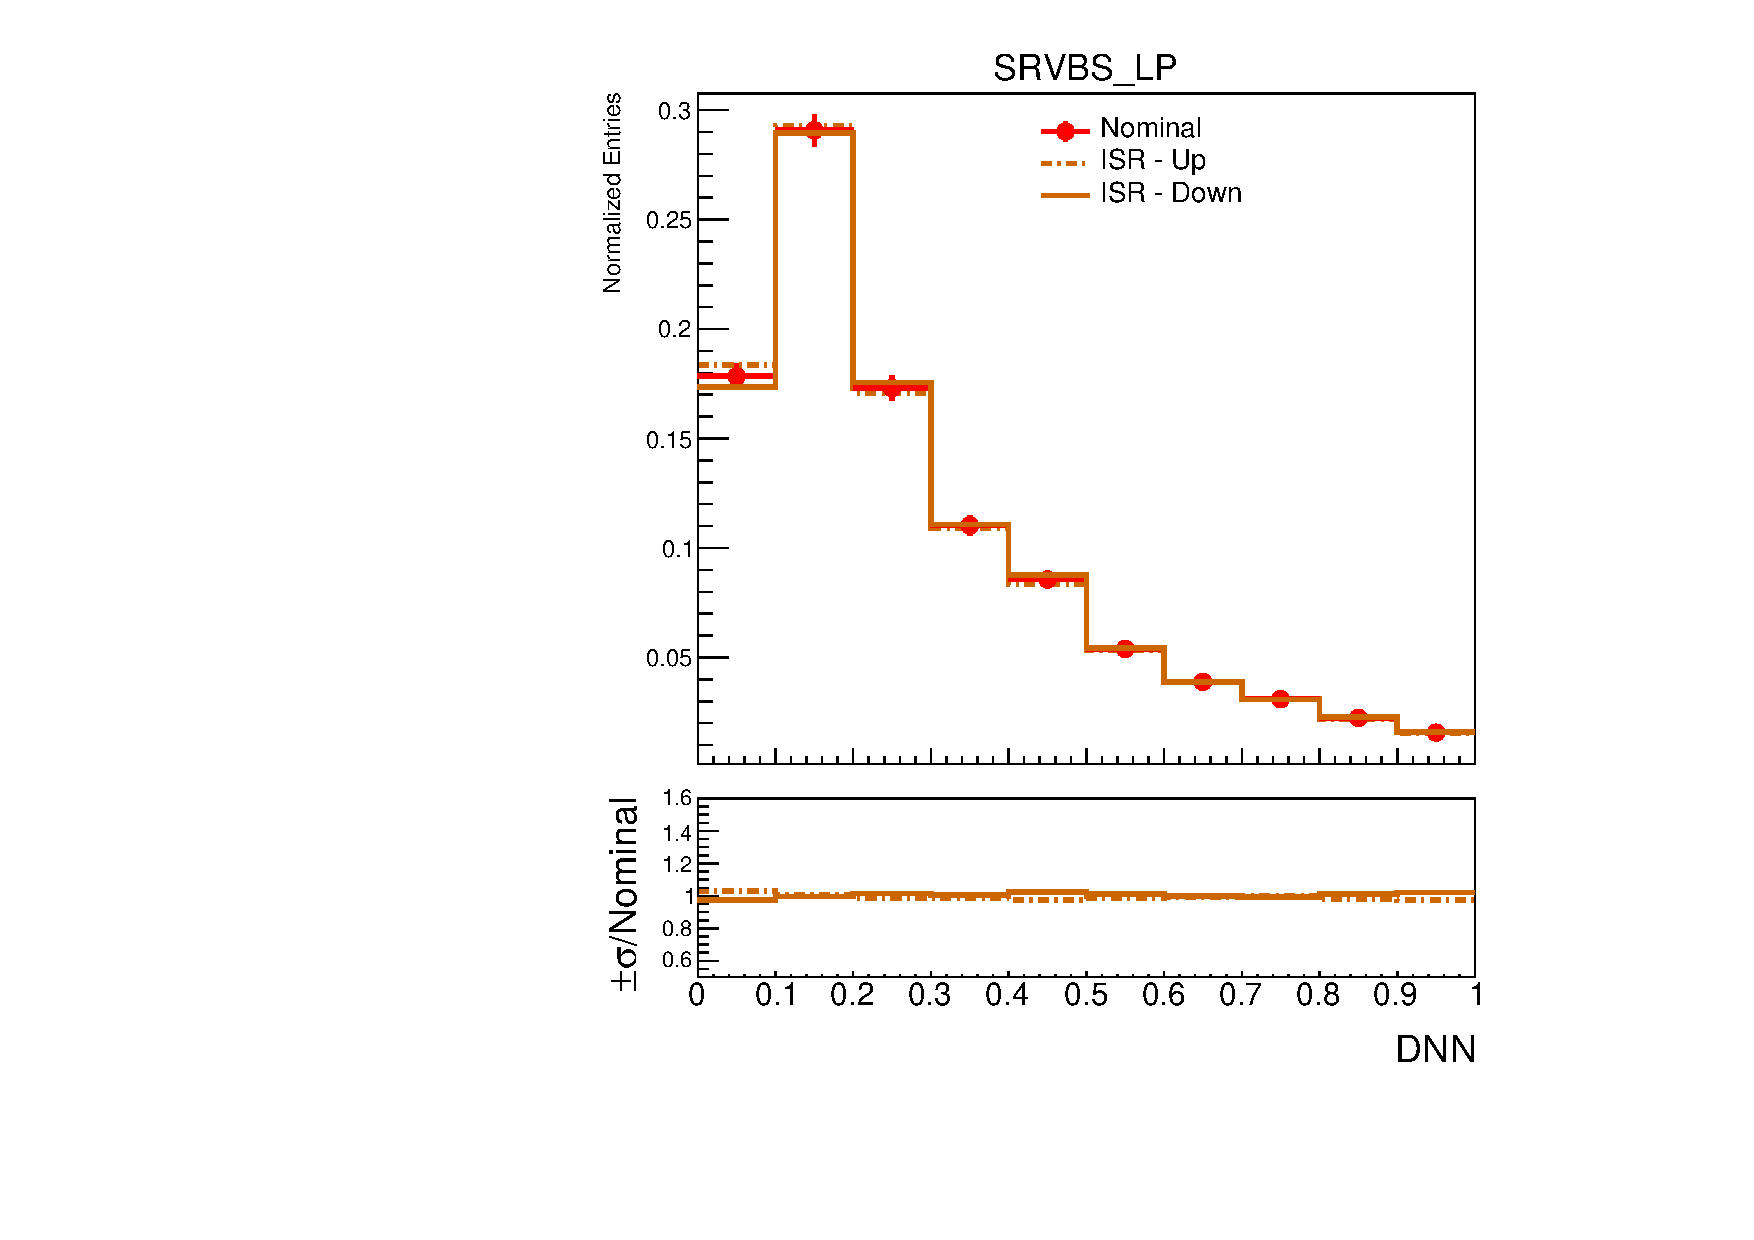
\includegraphics[width=\textwidth]{figures/1lep/PDFUnc/ISR/stopWt_0ptag1pfat0pjet_0ptv_SRVBS_LP_DNN_SysTheoryISR_stop__1up_Norm.pdf}
%%%        \caption{stopWt, merged LP SR}
%%%    \end{subfigure}
    \caption{ISR uncertainties in the 1-lepton channel.}
    \label{fig:isrUnc1Lep}
\end{figure}

\begin{figure}[p]
    \centering
    \begin{subfigure}[b]{0.3\textwidth}
        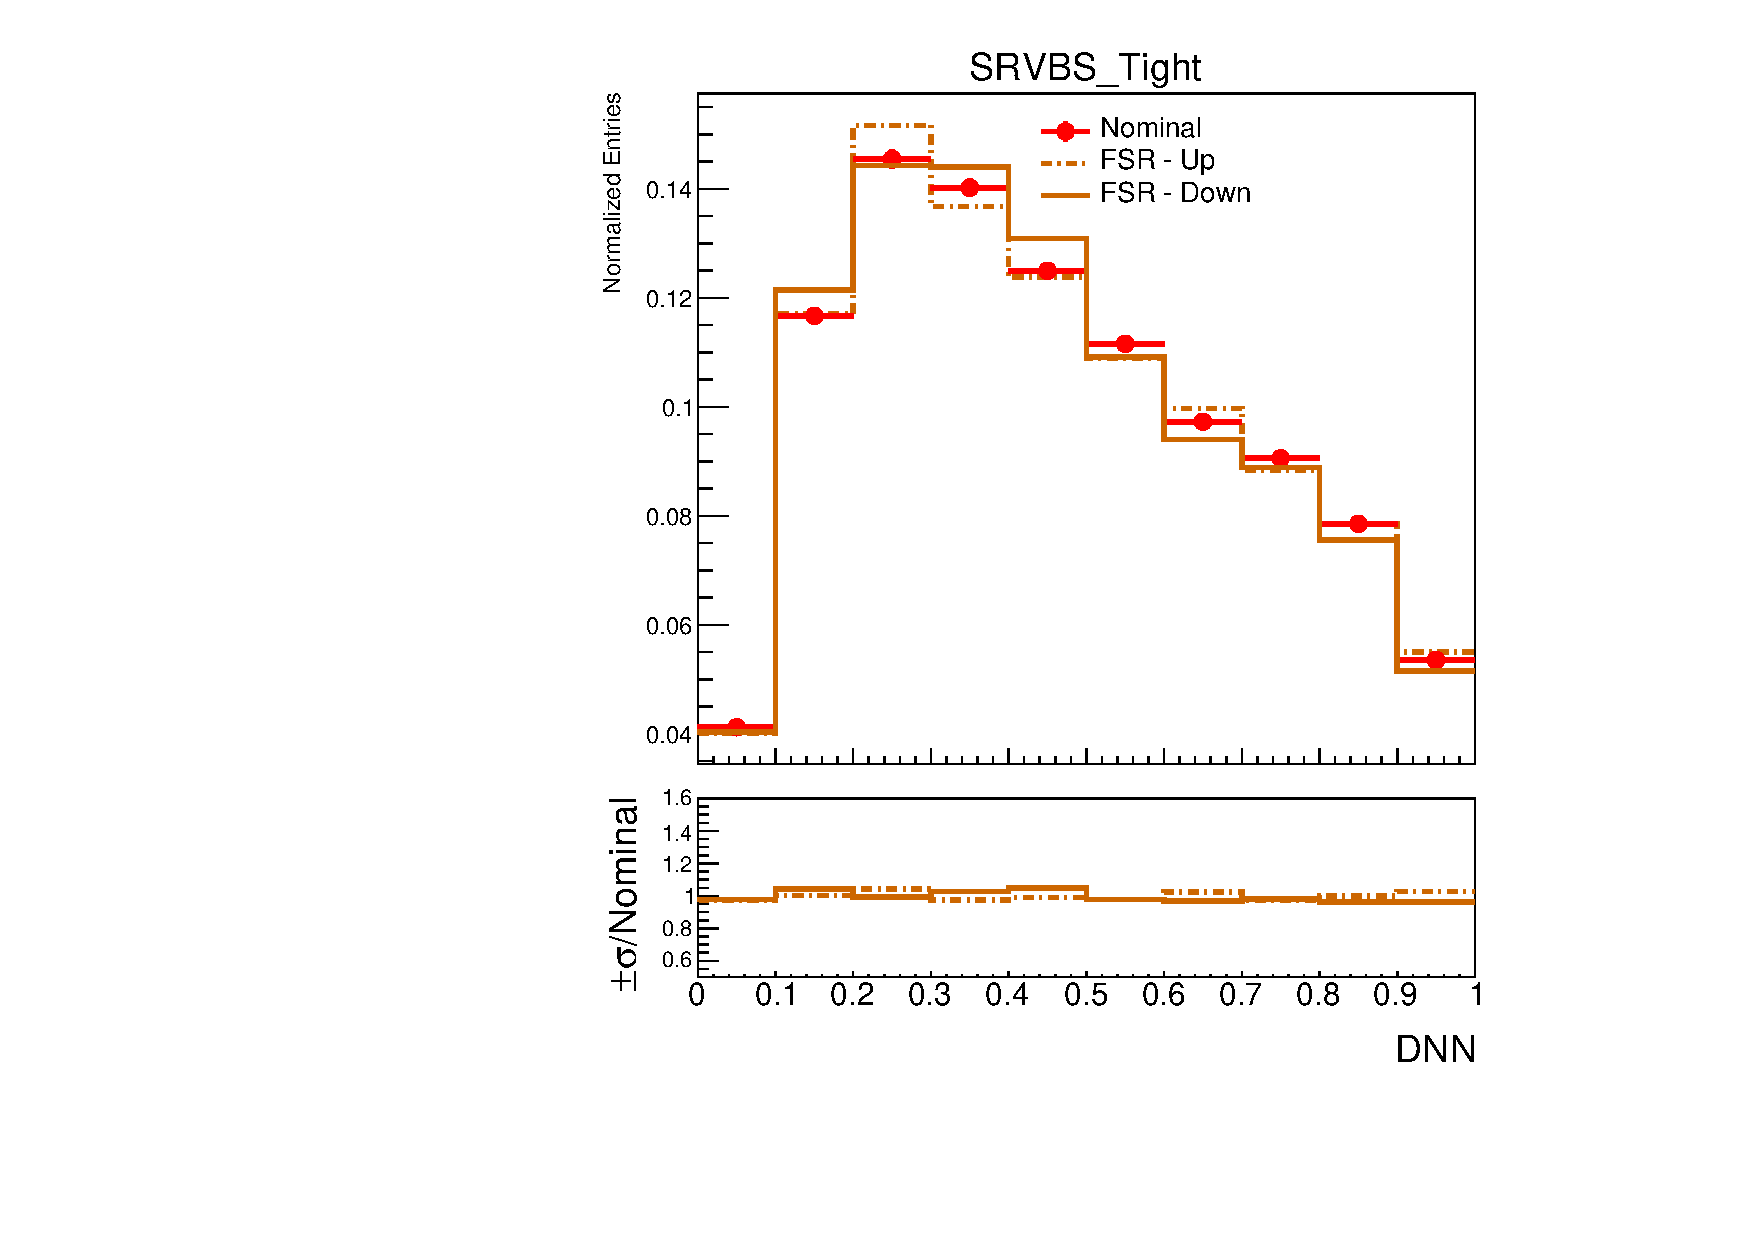
\includegraphics[width=\textwidth]{figures/1lep/PDFUnc/FSR/ttbar_0ptag2pjet_0ptv_SRVBS_Tight_DNN_SysTheoryFSR_Top__1up_Norm.pdf}
        \caption{\ttbar, resolved SR}
    \end{subfigure}
    \begin{subfigure}[b]{0.3\textwidth}
        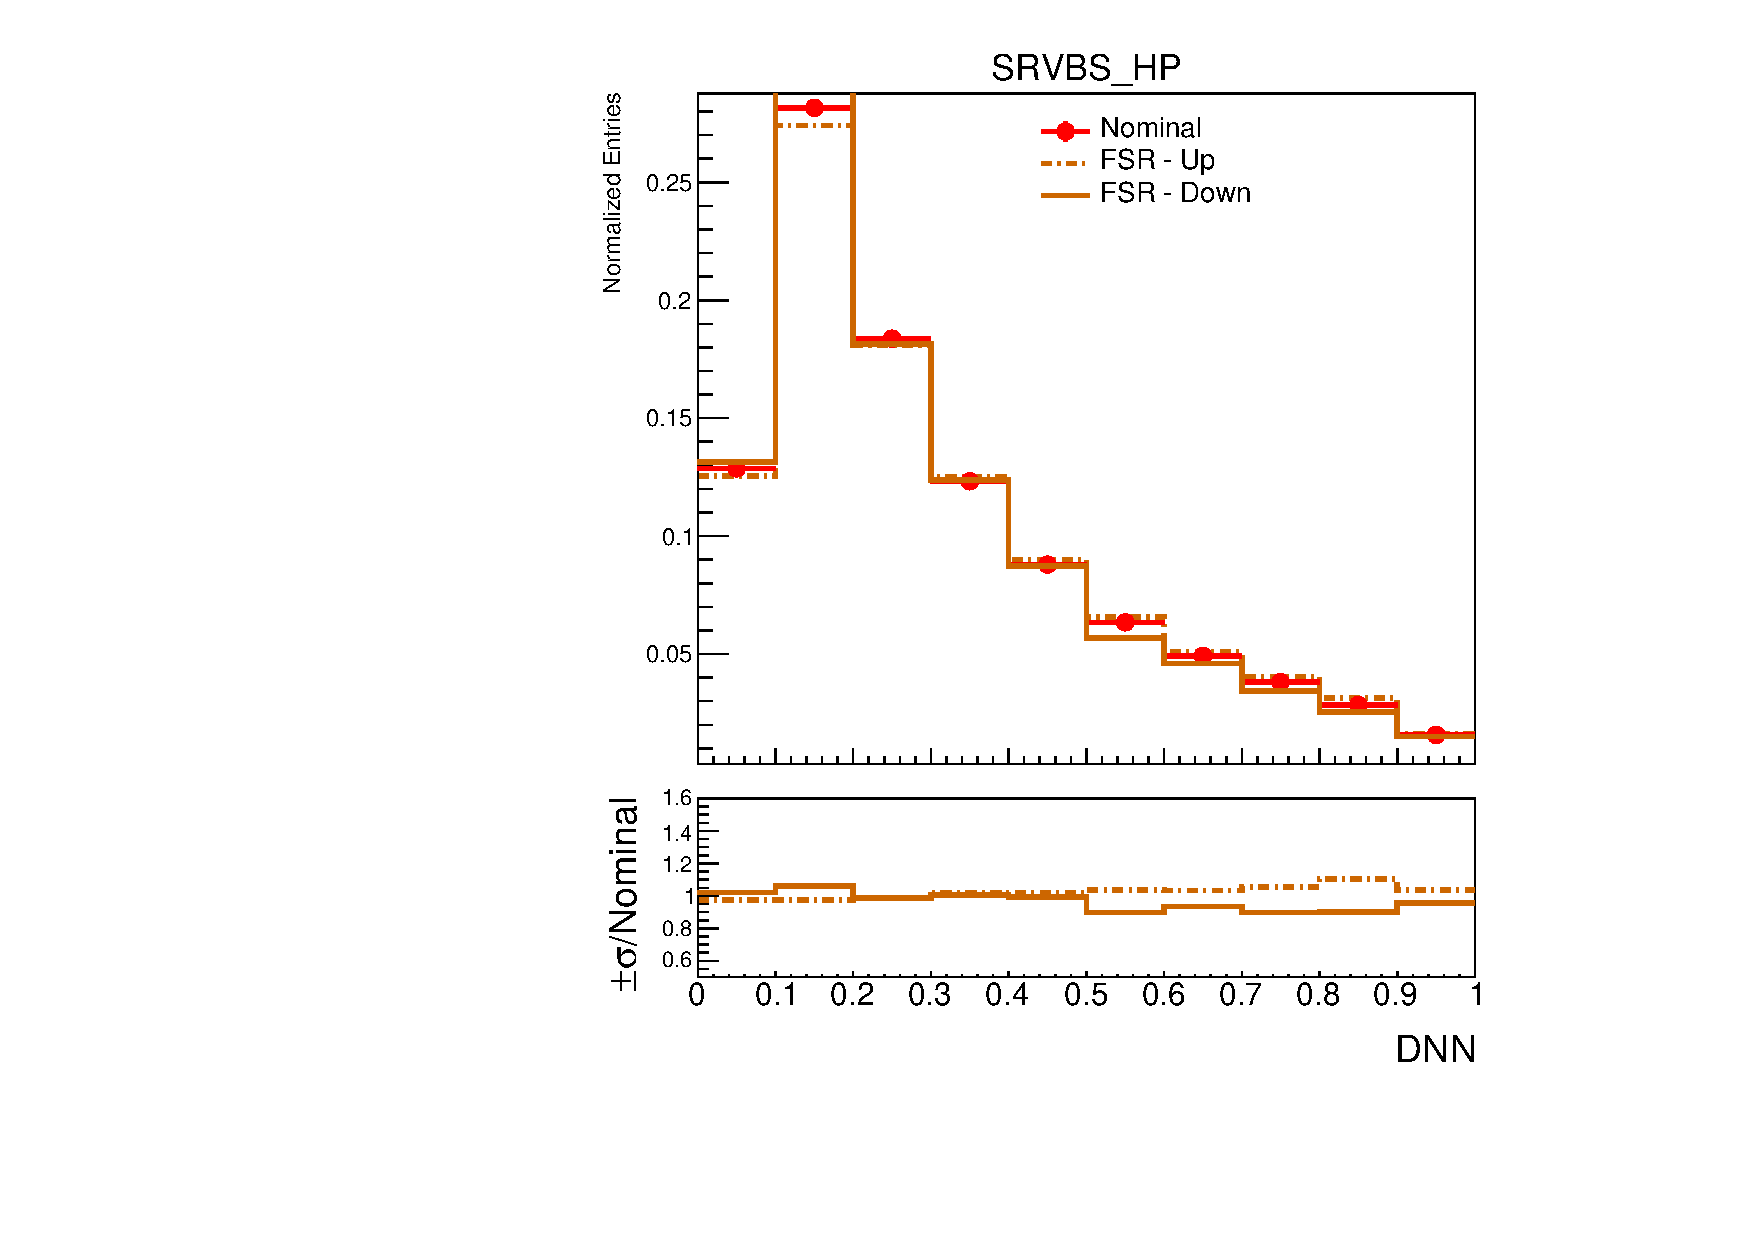
\includegraphics[width=\textwidth]{figures/1lep/PDFUnc/FSR/ttbar_0ptag1pfat0pjet_0ptv_SRVBS_HP_DNN_SysTheoryFSR_Top__1up_Norm.pdf}
        \caption{\ttbar, merged HP SR}
    \end{subfigure}
    \begin{subfigure}[b]{0.3\textwidth}
        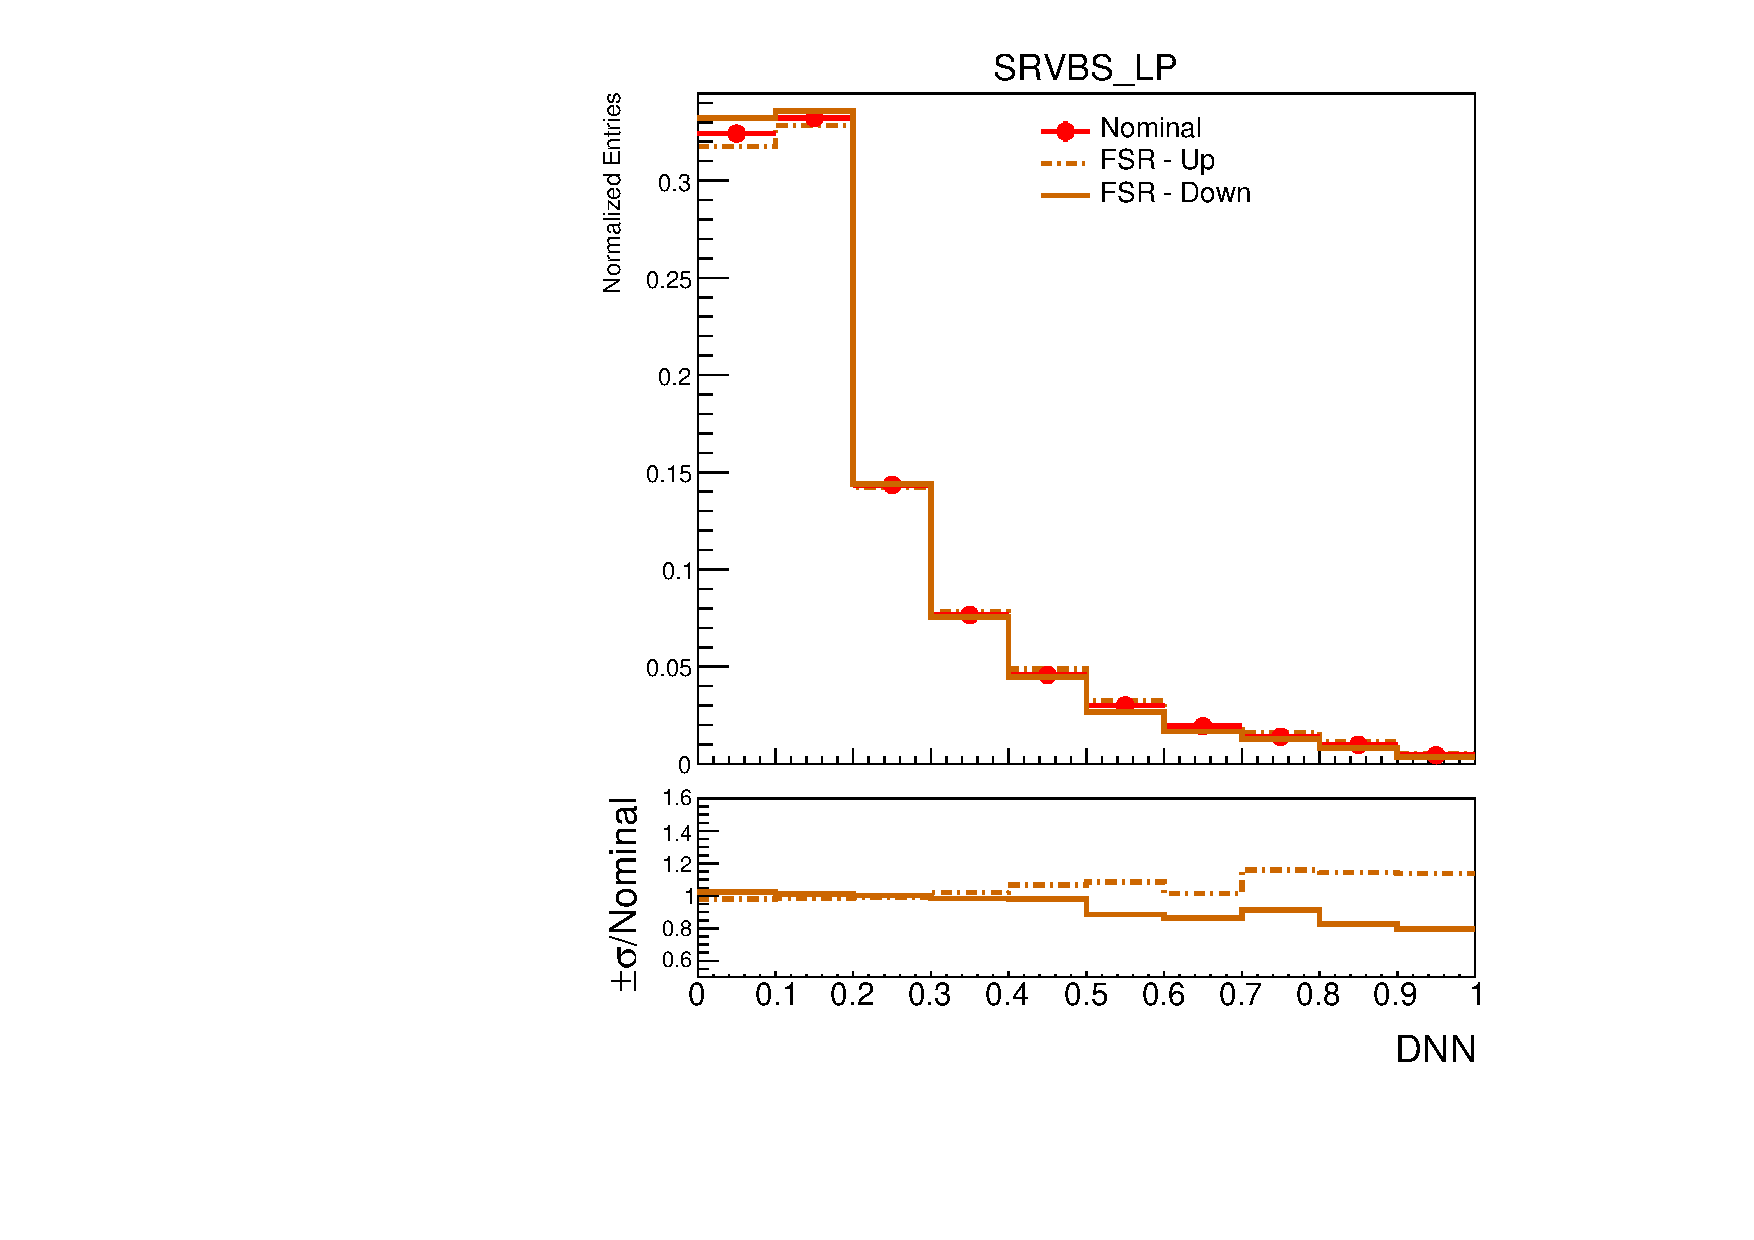
\includegraphics[width=\textwidth]{figures/1lep/PDFUnc/FSR/ttbar_0ptag1pfat0pjet_0ptv_SRVBS_LP_DNN_SysTheoryFSR_Top__1up_Norm.pdf}
        \caption{\ttbar, merged LP SR}
    \end{subfigure}
    \caption{FSR uncertainties in the 1-lepton channel.}
    \label{fig:fsrUnc1Lep}
\end{figure}

%%%%%%%%
\clearpage
\subsection{Tag Jets re-weighting}
\label{subsec:bkg_uncer_mjjrew}
%%As described in Sec. \ref{subsec:mjj_reweight}, a reweighting is applied to \Wjets and \Zjets as a function of \mjjtag.
%%We assign uncertainty for this reweighting considering a 100\% uncertainty on the linear fit parameters;
%%this uncertainty is considered as a modelling systematic for both \Wjets and \Zjets.

As outlined in Section \ref{subsec:mjj_reweight}, a reweighting procedure is applied to the \Wjets and \Zjets samples based on the \mjjtag variable. 
An uncertainty is assigned to this reweighting by assuming a 100\% uncertainty in the parameters of the linear fit. 
This is treated as a modelling systematic uncertainty for both \Wjets\ and \Zjets.


%%%%%
%%%%%The impact of \mjjtag re-weighting uncertainty on the final discriminant 
%%%%%is shown 
%%%%%in Figures \ref{fig:MjjUnc0LepWjets} - \ref{fig:MjjUnc0LepZjets} for the \zlep channel
%%%%%and 
%%%%%in Figures~\ref{fig:MjjUnc1LepCR} - \ref{fig:MjjUnc1LepSR} for the \olep channel.
%%%%%and 
%%%%%in Figures~\ref{fig:MjjUnc2LepCR} - \ref{fig:MjjUnc2LepSR} for the \tlep channel.
%%%%%
%%%%%\begin{figure}[ht]
%%%%%    \centering
%%%%%    	\subfigure[mjj: merged CR]{\includegraphics[width=0.32\textwidth]{figures/0lep/systematics/rewe/merged/plots/systreweWWjets_nom_MTagJets_CRVjet_Mer.pdf}}
%%%%%    	\subfigure[mjj: resolved CR]{\includegraphics[width=0.32\textwidth]{figures/0lep/systematics/rewe/merged/plots/systreweWWjets_nom_MTagJets_CRVjet_Fid.pdf}}\\
%%%%%    	\subfigure[mjj: merged HP SR]{\includegraphics[width=0.32\textwidth]{figures/0lep/systematics/rewe/merged/plots/systreweWWjets_nom_MTagJets_SRVBS_HP.pdf}}
%%%%%    	\subfigure[mjj: merged LP SR]{\includegraphics[width=0.32\textwidth]{figures/0lep/systematics/rewe/merged/plots/systreweWWjets_nom_MTagJets_SRVBS_LP.pdf}}
%%%%%    	\subfigure[mjj: resolved SR]{\includegraphics[width=0.32\textwidth]{figures/0lep/systematics/rewe/merged/plots/systreweWWjets_nom_MTagJets_SRVBS_Fid.pdf}}\\
%%%%%    	\subfigure[RNN: merged HP SR]{\includegraphics[width=0.32\textwidth]{figures/0lep/systematics/rewe/merged/plots/systreweWWjets_nom_RNN_SRVBS_HP.pdf}}
%%%%%    	\subfigure[RNN: merged LP SR]{\includegraphics[width=0.32\textwidth]{figures/0lep/systematics/rewe/merged/plots/systreweWWjets_nom_RNN_SRVBS_LP.pdf}}
%%%%%    	\subfigure[RNN: resolved SR]{\includegraphics[width=0.32\textwidth]{figures/0lep/systematics/rewe/merged/plots/systreweWWjets_nom_RNN_SRVBS_Fid.pdf}}\\
%%%%%        \caption{Nominal uncertainties from the mjj-reweighting process in the 0-lepton channel on the \Wjets background. Shown here are $m_{jj,tag}$ and RNN score distributions.} 
%%%%%    \label{fig:MjjUnc0LepWjets}
%%%%%\end{figure}
%%%%%\begin{figure}[ht]
%%%%%    \centering
%%%%%    	\subfigure[mjj: merged CR]{\includegraphics[width=0.32\textwidth]{figures/0lep/systematics/rewe/merged/plots/systreweZZjets_nom_MTagJets_CRVjet_Mer.pdf}}
%%%%%    	\subfigure[mjj: resolved CR]{\includegraphics[width=0.32\textwidth]{figures/0lep/systematics/rewe/merged/plots/systreweZZjets_nom_MTagJets_CRVjet_Fid.pdf}}\\
%%%%%    	\subfigure[mjj: merged HP SR]{\includegraphics[width=0.32\textwidth]{figures/0lep/systematics/rewe/merged/plots/systreweZZjets_nom_MTagJets_SRVBS_HP.pdf}}
%%%%%    	\subfigure[mjj: merged LP SR]{\includegraphics[width=0.32\textwidth]{figures/0lep/systematics/rewe/merged/plots/systreweZZjets_nom_MTagJets_SRVBS_LP.pdf}}
%%%%%    	\subfigure[mjj: resolved SR]{\includegraphics[width=0.32\textwidth]{figures/0lep/systematics/rewe/merged/plots/systreweZZjets_nom_MTagJets_SRVBS_Fid.pdf}}\\
%%%%%    	\subfigure[RNN: merged HP SR]{\includegraphics[width=0.32\textwidth]{figures/0lep/systematics/rewe/merged/plots/systreweZZjets_nom_RNN_SRVBS_HP.pdf}}
%%%%%    	\subfigure[RNN: merged LP SR]{\includegraphics[width=0.32\textwidth]{figures/0lep/systematics/rewe/merged/plots/systreweZZjets_nom_RNN_SRVBS_LP.pdf}}
%%%%%    	\subfigure[RNN: resolved SR]{\includegraphics[width=0.32\textwidth]{figures/0lep/systematics/rewe/merged/plots/systreweZZjets_nom_RNN_SRVBS_Fid.pdf}}\\
%%%%%        \caption{Nominal uncertainties from the mjj-reweighting process in the 0-lepton channel on the \Wjets background. Shown here are $m_{jj,tag}$ and RNN score distributions.} 
%%%%%    \label{fig:MjjUnc0LepZjets}
%%%%%\end{figure}
%%%%%
%%%%%
%%%%%\begin{figure}[ht]
%%%%%    \centering
%%%%%	\subfigure[\mjjtag reweighting uncertainties for mjjtag in the Wjets resolved control region]{\includegraphics[width=0.45\textwidth]{figures/1lep/MjjUnc/SystMJJCRVjetsResTight_W_tagMjj.pdf}}
%%%%%	\subfigure[\mjjtag reweighting uncertainties for RNN score in the Wjets resolved control region]{\includegraphics[width=0.45\textwidth]{figures/1lep/MjjUnc/SystMJJCRVjetsResTight_W_RNN.pdf}}
%%%%%	\subfigure[\mjjtag reweighting uncertainties for mjjtag in the Wjets merged control region]{\includegraphics[width=0.45\textwidth]{figures/1lep/MjjUnc/SystMJJCRVjetsMerged_W_tagMjj.pdf}}
%%%%%	\subfigure[\mjjtag reweighting uncertainties for RNN score in the Wjets merged control region]{\includegraphics[width=0.45\textwidth]{figures/1lep/MjjUnc/SystMJJCRVjetsMerged_W_RNN.pdf}}
%%%%%	\caption{Nominal uncertainties from the mjj-reweighting process in the 1-lepton channel. Shown here are $m_{jj,tag}$ and RNN score distributions in CRs. In particular, the legend of the figure refers to the uncertainty coming from the fit parameters as the 'Nominal' and to the 100\% one as the 'Conservative'; the 'Conservative' one is the one used in the results as for the other channels.}
%%%%%    \label{fig:MjjUnc1LepCR}
%%%%%\end{figure}
%%%%%
%%%%%\begin{figure}[ht]
%%%%%    \centering
%%%%% 	\subfigure[\mjjtag reweighting uncertainties for mjjtag in the resolved signal region]{\includegraphics[width=0.45\textwidth]{figures/1lep/MjjUnc/SystMJJSRResTight_W_tagMjj.pdf}}
%%%%% 	\subfigure[\mjjtag reweighting uncertainties for RNN score in the resolved signal region]{\includegraphics[width=0.45\textwidth]{figures/1lep/MjjUnc/SystMJJSRResTight_W_RNN.pdf}}
%%%%%        \subfigure[\mjjtag reweighting uncertainties for mjjtag in the merged HP signal region]{\includegraphics[width=0.45\textwidth]{figures/1lep/MjjUnc/SystMJJSRHP_W_tagMjj.pdf}}
%%%%%        \subfigure[\mjjtag reweighting uncertainties for RNN score in the merged HP signal region]{\includegraphics[width=0.45\textwidth]{figures/1lep/MjjUnc/SystMJJSRHP_W_RNN.pdf}}
%%%%%        \subfigure[\mjjtag reweighting uncertainties for mjjtag in the merged LP signal region]{\includegraphics[width=0.45\textwidth]{figures/1lep/MjjUnc/SystMJJSRLP_W_tagMjj.pdf}}
%%%%%        \subfigure[\mjjtag reweighting uncertainties for RNN score in the merged LP signal region]{\includegraphics[width=0.45\textwidth]{figures/1lep/MjjUnc/SystMJJSRLP_W_RNN.pdf}}
%%%%%	\caption{Nominal uncertainties from the mjj-reweighting process in the 1-lepton channel. Shown here are $m_{jj,tag}$ and RNN score distributions in SRs. In particular, the legend of the figure refers to the uncertainty coming from the fit parameters as the 'Nominal' and to the 100\% one as the 'Conservative'; the 'Conservative' one is the one used in the results as for the other channels.}
%%%%%    \label{fig:MjjUnc1LepSR}
%%%%%\end{figure}
%%%%%
%%%%%%2lep
%%%%%\begin{figure}[ht]
%%%%%    \centering
%%%%%	\subfigure[\mjjtag reweighting uncertainties for mjjtag in the Zjets resolved control region]{\includegraphics[width=0.32\textwidth]{figures/2lep/reweighting/Z_0ptag2pjet_0ptv_CRVjet_Fid_MTagResJets_SysMJJREWEIGHT_100per.pdf}}
%%%%%	\subfigure[\mjjtag reweighting uncertainties for RNN score in the Zjets resolved control region]{\includegraphics[width=0.32\textwidth]{figures/2lep/reweighting/Z_0ptag2pjet_0ptv_CRVjet_Fid_RNNScoreResolved_SysMJJREWEIGHT_100per.pdf}}
%%%%%	\subfigure[\mjjtag reweighting uncertainties for mjjtag in the Zjets merged control region]{\includegraphics[width=0.32\textwidth]{figures/2lep/reweighting/Z_0ptag1pfat0pjet_0ptv_CRVjet_MTagMerJets_SysMJJREWEIGHT_100per.pdf}}
%%%%%	\subfigure[\mjjtag reweighting uncertainties for RNN score in the Zjets merged control region]{\includegraphics[width=0.32\textwidth]{figures/2lep/reweighting/Z_0ptag1pfat0pjet_0ptv_CRVjet_RNNScoreMerged_SysMJJREWEIGHT_100per.pdf}}
%%%%%	\caption{Nominal uncertainties from the mjj-reweighting process in the 2-lepton channel. Shown here are $m_{jj,tag}$ and RNN score distributions in CRs. }
%%%%%    \label{fig:MjjUnc2LepCR}
%%%%%\end{figure}
%%%%%
%%%%%\begin{figure}[ht]
%%%%%    \centering
%%%%% 	\subfigure[\mjjtag reweighting uncertainties for mjjtag in the resolved signal region]{\includegraphics[width=0.32\textwidth]{figures/2lep/reweighting/Z_0ptag2pjet_0ptv_SRVBS_Fid_MTagResJets_SysMJJREWEIGHT_100per.pdf}}
%%%%% 	\subfigure[\mjjtag reweighting uncertainties for RNN score in the resolved signal region]{\includegraphics[width=0.32\textwidth]{figures/2lep/reweighting/Z_0ptag2pjet_0ptv_SRVBS_Fid_RNNScoreResolved_SysMJJREWEIGHT_100per.pdf}}
%%%%%        \subfigure[\mjjtag reweighting uncertainties for mjjtag in the merged HP signal region]{\includegraphics[width=0.32\textwidth]{figures/2lep/reweighting/Z_0ptag1pfat0pjet_0ptv_SRVBS_HP_MTagMerJets_SysMJJREWEIGHT_100per.pdf}}
%%%%%        \subfigure[\mjjtag reweighting uncertainties for RNN score in the merged HP signal region]{\includegraphics[width=0.32\textwidth]{figures/2lep/reweighting/Z_0ptag1pfat0pjet_0ptv_SRVBS_HP_RNNScoreMerged_SysMJJREWEIGHT_100per.pdf}}
%%%%%        \subfigure[\mjjtag reweighting uncertainties for mjjtag in the merged LP signal region]{\includegraphics[width=0.32\textwidth]{figures/2lep/reweighting/Z_0ptag1pfat0pjet_0ptv_SRVBS_LP_MTagMerJets_SysMJJREWEIGHT_100per.pdf}}
%%%%%        \subfigure[\mjjtag reweighting uncertainties for RNN score in the merged LP signal region]{\includegraphics[width=0.32\textwidth]{figures/2lep/reweighting/Z_0ptag1pfat0pjet_0ptv_SRVBS_LP_RNNScoreMerged_SysMJJREWEIGHT_100per.pdf}}
%%%%%	\caption{Nominal uncertainties from the mjj-reweighting process in the 2-lepton channel. Shown here are $m_{jj,tag}$ and RNN score distributions in SRs. }
%%%%%    \label{fig:MjjUnc2LepSR}
%%%%%\end{figure}

